\chapter{Opis danych}
\label{chap:opisdanych}
Pierwszym korkiem w celu przeprowadzenia eksperymentów było zdobycie odpowiednich danych wejściowych. Zadanie to było proste, gdyż otrzymaliśmy dostęp do zbioru danych, wytworzonego w trakcie pracy, na której bazujemy naszą tezę \cite{DBLP:conf/sigmod/BodzionyKPW21}. Znaleźć je można na repozytorium w serwisie GitHub.com utworzonym przez autorów poprzedniej pracy\footnote{\url{https://github.com/pientaa/spark-udf-characteristics}}.
Dane te zostały zebrane podczas przetwarzania w środowisku Apache Spark z każdego skonfigurowanego węzła i zapisane w formacie CSV w odpowiednim folderze. W sumie otrzymaliśmy 33,600 surowych plików, gdzie każdy plik to osobny przebieg wykonywania się funkcji.Struktura tych danych prezentuje się następująco:\\ 
\noindent'$<$typ przetwarzania$>$/$<$nazwa UDF$>$/$<$konfiguracja klastra$>$/source-data/node-$<$id węzła$>$/$<$data uruchomienia$>$.csv'\\
przykładowo:
\begin{figure}[H]
    \centering
    \captionsetup{justification=centering,margin=0.5cm}
    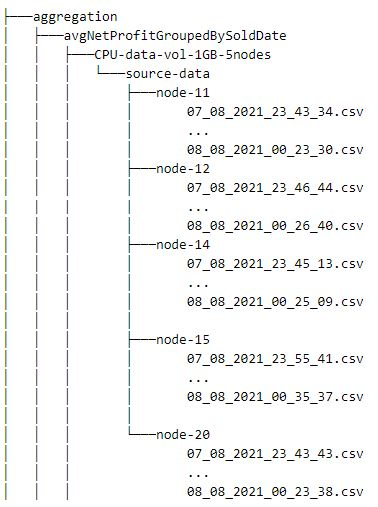
\includegraphics[scale=0.8]{figures/04-opis-danych/folder_structure.JPG}
    \caption{Struktura surowych danych}
    \label{fig:raw_file_structure}
\end{figure}
Każda funkcja została uruchomiona 25 razy per konfiguracja klastra. W każdym węźle zawarte są informacje o zużyciu procesora i pamięci RAM w trakcie wykonywania się UDF'a dla utworzonych procesów. Z tego powodu dla jednego momentu w czasie może być zaraportowanych parę procesów z ich zużyciem zasobów. Wszystko to jest zebrane w pliku CSV o następującym schemacie:
\begin{itemize}
    \item timestamp - znacznik czasowy w formacie 'rok-miesiąc-dzień godzina:minuta:sekunda.milisekunda'.
    \item PID - identyfikator procesu.
    \item CPU - procent zużycia procesora przez proces, dla zadań wielordzeniowych może przekroczyć 100\%.
    \item RAM - procent zużycia pamięci przez proces.
\end{itemize}
\section{Wstępne przetwarzanie danych}
Dane w tym stanie nie nadają się do eksperymentów, więc wpierw należało je uporządkować i zapisać w wygodnym dla nas formacie. Wpierw konieczne było pozbycie się podziału na procesy. Dla nas najbardziej interesujący jest sumaryczny przebieg zużycia zasobów na poziomie całej funkcji, a niż poszczególnych procesów. W tym celu wykorzystaliśmy bibliotekę \textbf{Pandas} \cite{reback2020pandas} często wykorzystywaną w przetwarzaniu danych \cite{reback2020pandas}. Wpisy zostały pogrupowane po znacznikach czasowych, następnie procenty zużycia zasobów (kolumny CPU oraz RAM) zsumowane w ramach jednej grupy. Jeszcze należało usunąć identyfikatory procesów, gdyż nie są one nam potrzebne do dalszego przetwarzania. Dodatkowo kolumna 'timestamp' zastąpiona jest kolumną 'epoch', która opisuje liczbę sekund (z dokładnością do 16 miejsc po przecinku) która minęła od uruchomienia funkcji.

Otrzymane zbiory zostały zapisane w takiej samej strukturze jak wcześniej, ale w osobnym nad-folderze 'Prepared'.

W dalszym ciągu pozostaje kwestia zawartości poszczególnych folderów węzłów. Dla każdego uruchomienia funkcji posiadamy przebiegi o zużyciu w każdym węźle, zamiast ogólnie dla UDF'a. Dodatkowo bazując na pracy pilotażowej, wiemy że nie każdy węzeł aktywnie brał udział w obliczeniach. Jeden z węzłów był zawsze używany jako master, którego zadaniem było zarządzanie wykonywaniem się zadań na klastrach pracujących (workers). Jeżeli master nie nadał zadania każdemu z klastrów pracujących, to taki węzeł nic nie robił poza wysyłaniem okazyjnie informacji o stanie (tzn. czy jest wciąż aktywny). Z tego powodu następnym krokiem było odfiltrowanie wszystkich węzłów bezczynnych oraz mastera i zachowanie jednie tych, które wykonywały jakieś obliczenia.

Założyliśmy, że master, ze względu na to, że nie wykonuje pracy na danych, nie powinien wykorzystywać zbyt dużo pamięci RAM. Rzeczywiście dla każdego eksperymentu można było znaleźć jeden węzeł, którego średnie zużycie RAM było wyraźnie mniejsze. Eksperymentując, ustaliliśmy próg 2\% - odrzuciliśmy wszystkie węzły, dla których średnie zużycie RAM było poniżej tego progu.

Następnym krokiem było znalezienie i wykluczenie węzłów niepracujących. Jako, że takie węzły wysyłały tylko okazyjne informacje o tym, że wciąż są aktywne to różnice między zużyciem CPU dla nich i dla węzłów pracujących również były wyraźnie widoczne. Dokładnie to było widać zwłaszcza w kilku początkowych pomiarach, które dla węzłów pracujących charakteryzowały się wysokim zużyciem CPU, co było dokładnie opisane i wytłumaczone w pracy pilotażowej. Z tego względu odrzuciliśmy węzły, których początkowe pomiary były niskie.

Ostatecznie chcieliśmy również uzyskać jak najmniej plików wejściowych, aby ułatwić dalsze przetwarzanie danych. Inspirując się przykładowym zbiorem danych wykorzystywanym do uczenia maszynowego na danych typu Time Series, utworzyliśmy pojedyncze pliki CSV per typ funkcji UDF o następującym schemacie:
\begin{itemize}
    \item snapshot - identyfikator pojedynczego przebiegu czasowego.
    \item label - opis typu funkcji, np 'aggregation'.
    \item udf - nazwa funkcji z którego pochodzi danych przebieg czasowy.
    \item epoch - liczba sekund, która minęła od uruchomienia się funkcji z dokładnością do 16 miejsc po przecinku.
    \item CPU - procent zużycia procesora przez proces, dla zadań wielordzeniowych może przekroczyć 100\%.
    \item RAM - procent zużycia pamięci przez proces.
\end{itemize}
Poniżej znajduje się przykładowe parę wierszy z tak utworzonego pliku dla funkcji typu 'aggregation':
\begin{table}[H]
\center{
 \begin{tabular}{|c|c|c|c|c|c|} 
 \hline
snapshot & label & udf & epoch & CPU & RAM \\
\hline
0 & aggregation & avgNetProfitGroupedBySoldDate & 0.0 & 206.7 & 4.8 \\
\hline
0 & aggregation & avgNetProfitGroupedBySoldDate & 0.1562700271606445 & 220.0 & 5.0 \\
\hline
0 & aggregation & avgNetProfitGroupedBySoldDate & 0.3140101432800293 & 133.3 & 5.19 \\
\hline
0 & aggregation & avgNetProfitGroupedBySoldDate & 0.4715931415557861 & 146.7 & 5.3 \\
\hline
0 & aggregation & avgNetProfitGroupedBySoldDate & 0.6280381679534912 & 126.7 & 5.4 \\
\hline
0 & aggregation & avgNetProfitGroupedBySoldDate & 0.7846581935882568 & 160.0 & 5.5 \\
\hline
\end{tabular}
}
\caption{Początek pliku joined\_aggregation.csv}
\end{table}

Zebrane tak dane mogą zostać użyte w dalszym przetwarzaniu. W zbiorze możemy wyróżnić pięć typów funkcji zależnie od rodzaju przetwarzania:
\begin{itemize}
    \item aggregation
    \item filtration
    \item filtration-aggregation
    \item filtration-aggregation-join
    \item filtration-join
\end{itemize}
Kolumna 'label' zawiera jedną z tych wartości, poniżej w celu przedstawienia przykładowych przebiegów czasowych narysowane są wykresy dla każdego z typów z podziałem na RAM i CPU.

\begin{figure}[H]
  \centering
  \subfloat[CPU]{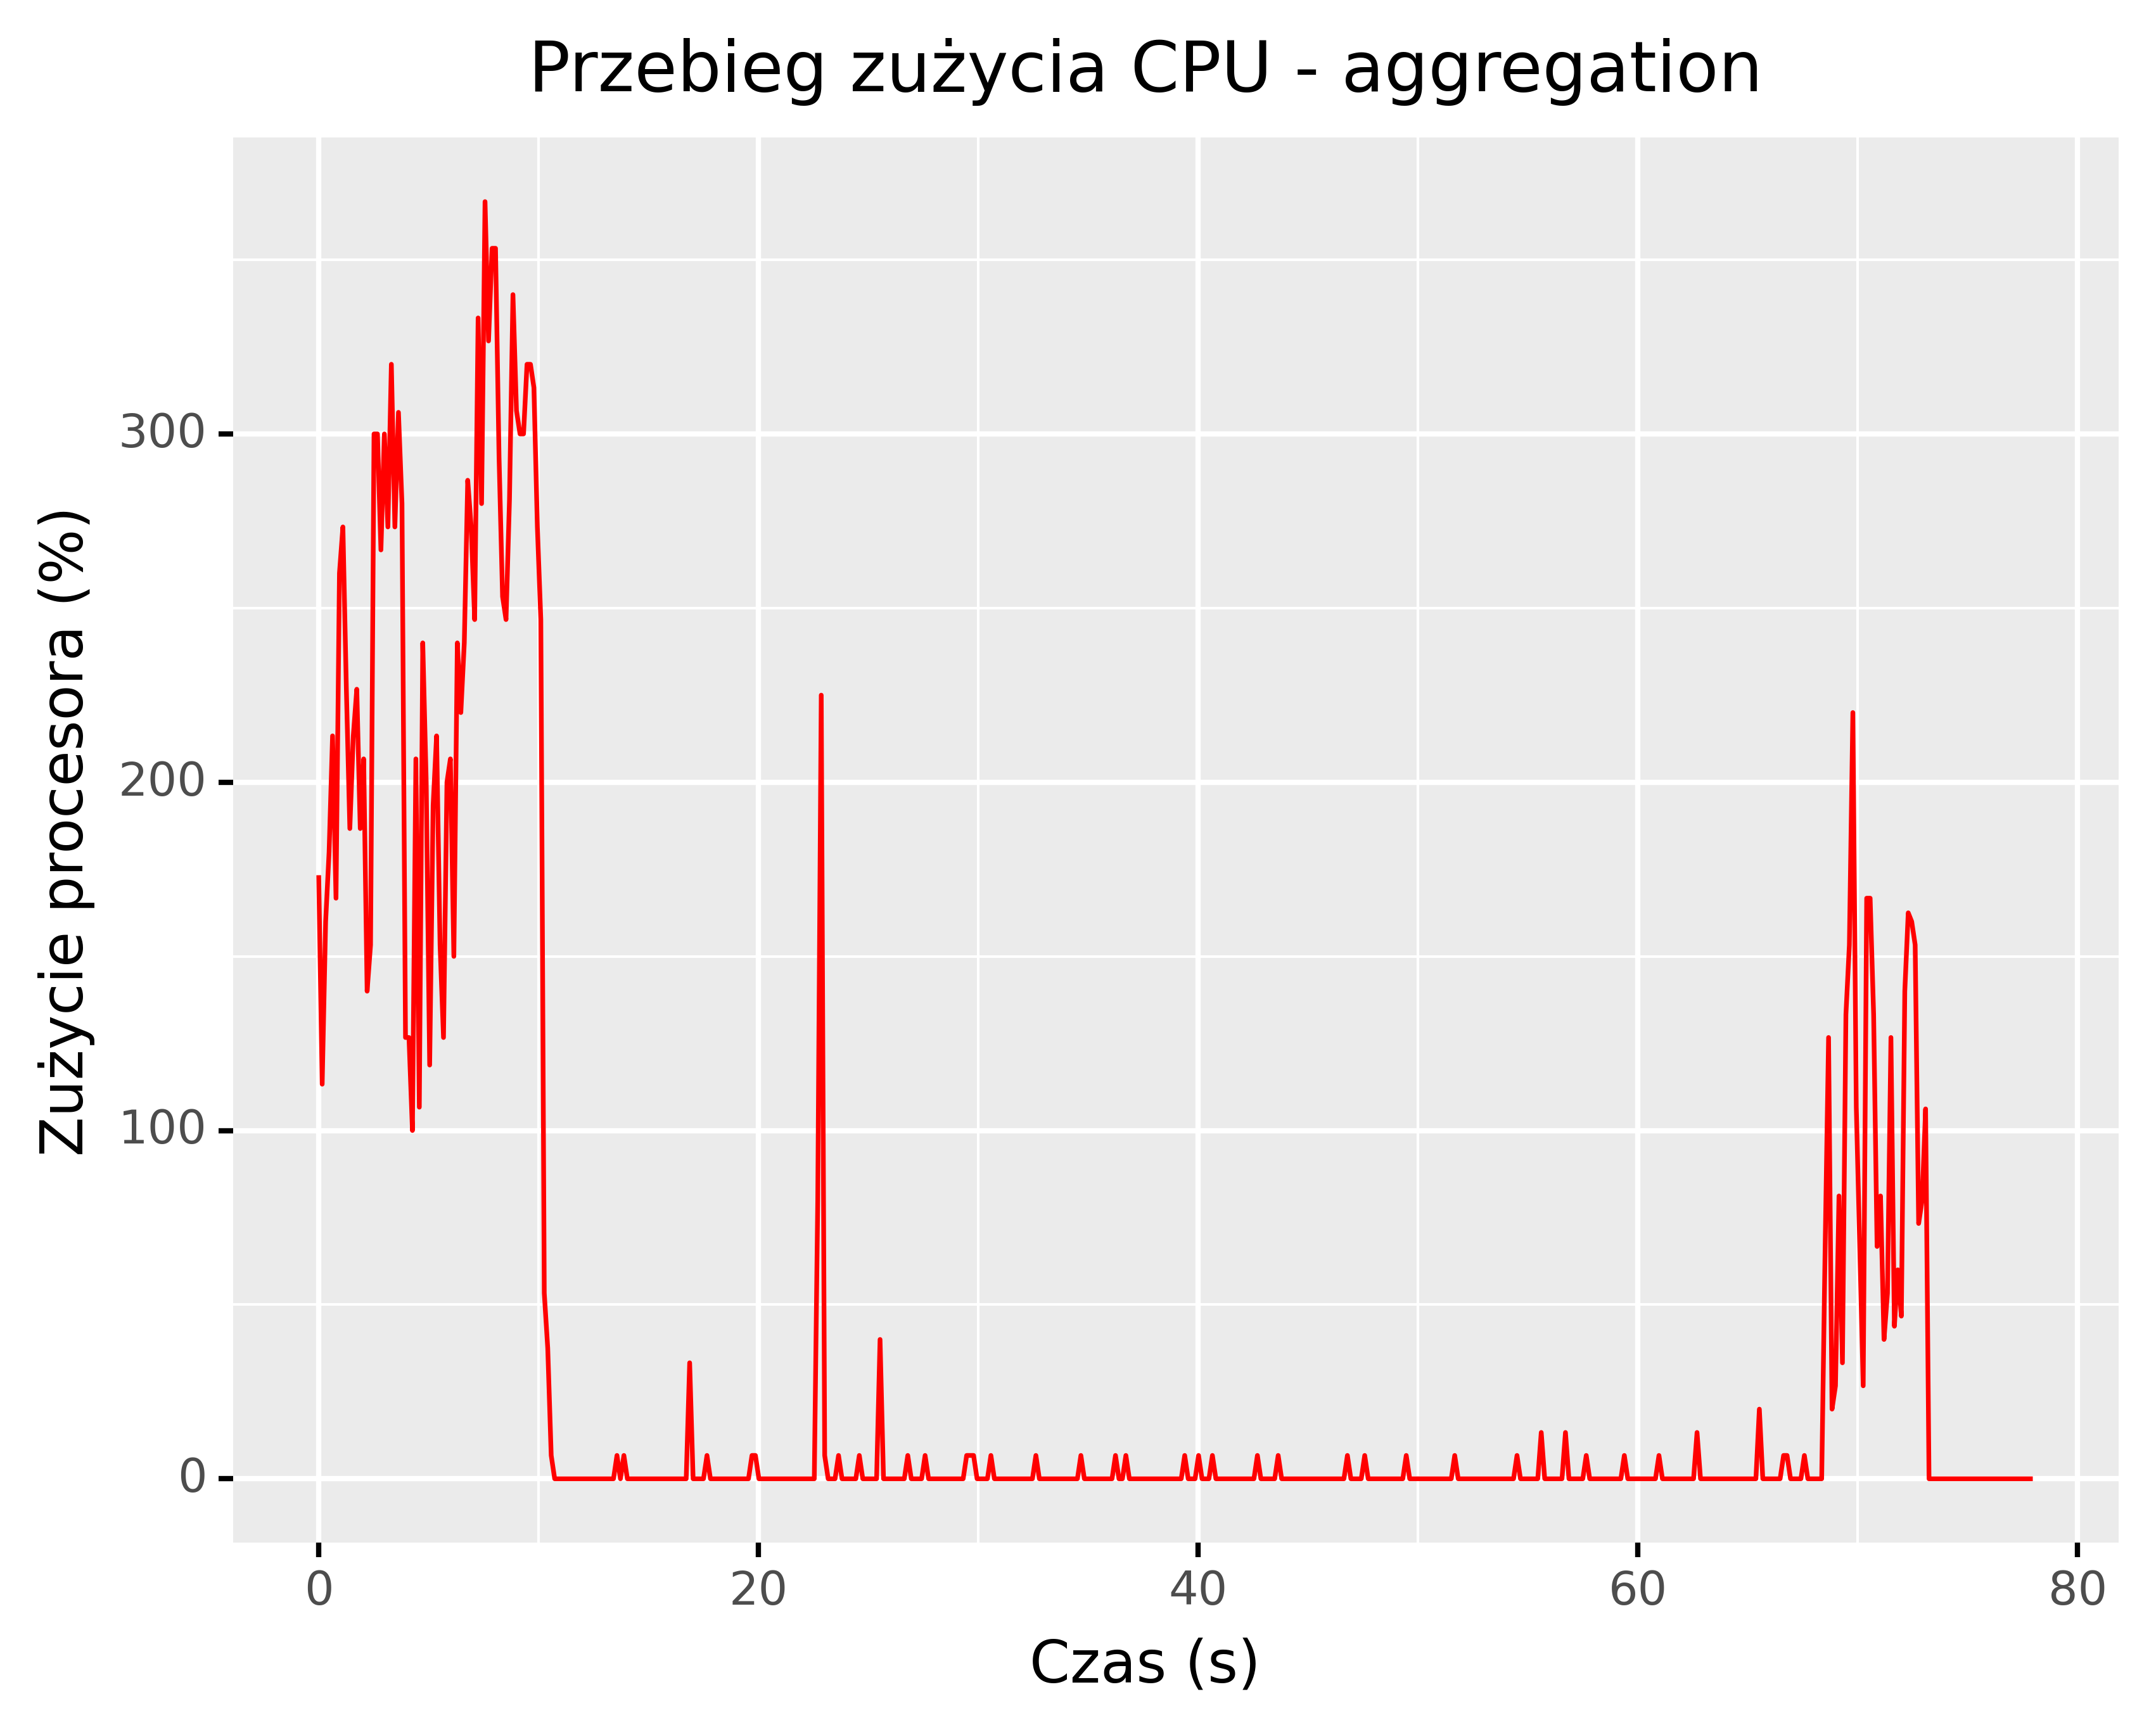
\includegraphics[width=0.5\textwidth]{figures/04-opis-danych/aggregation_example_cpu_snapshot_1.png}\label{aggregation_example:f1}}
  \hfill
  \subfloat[RAM]{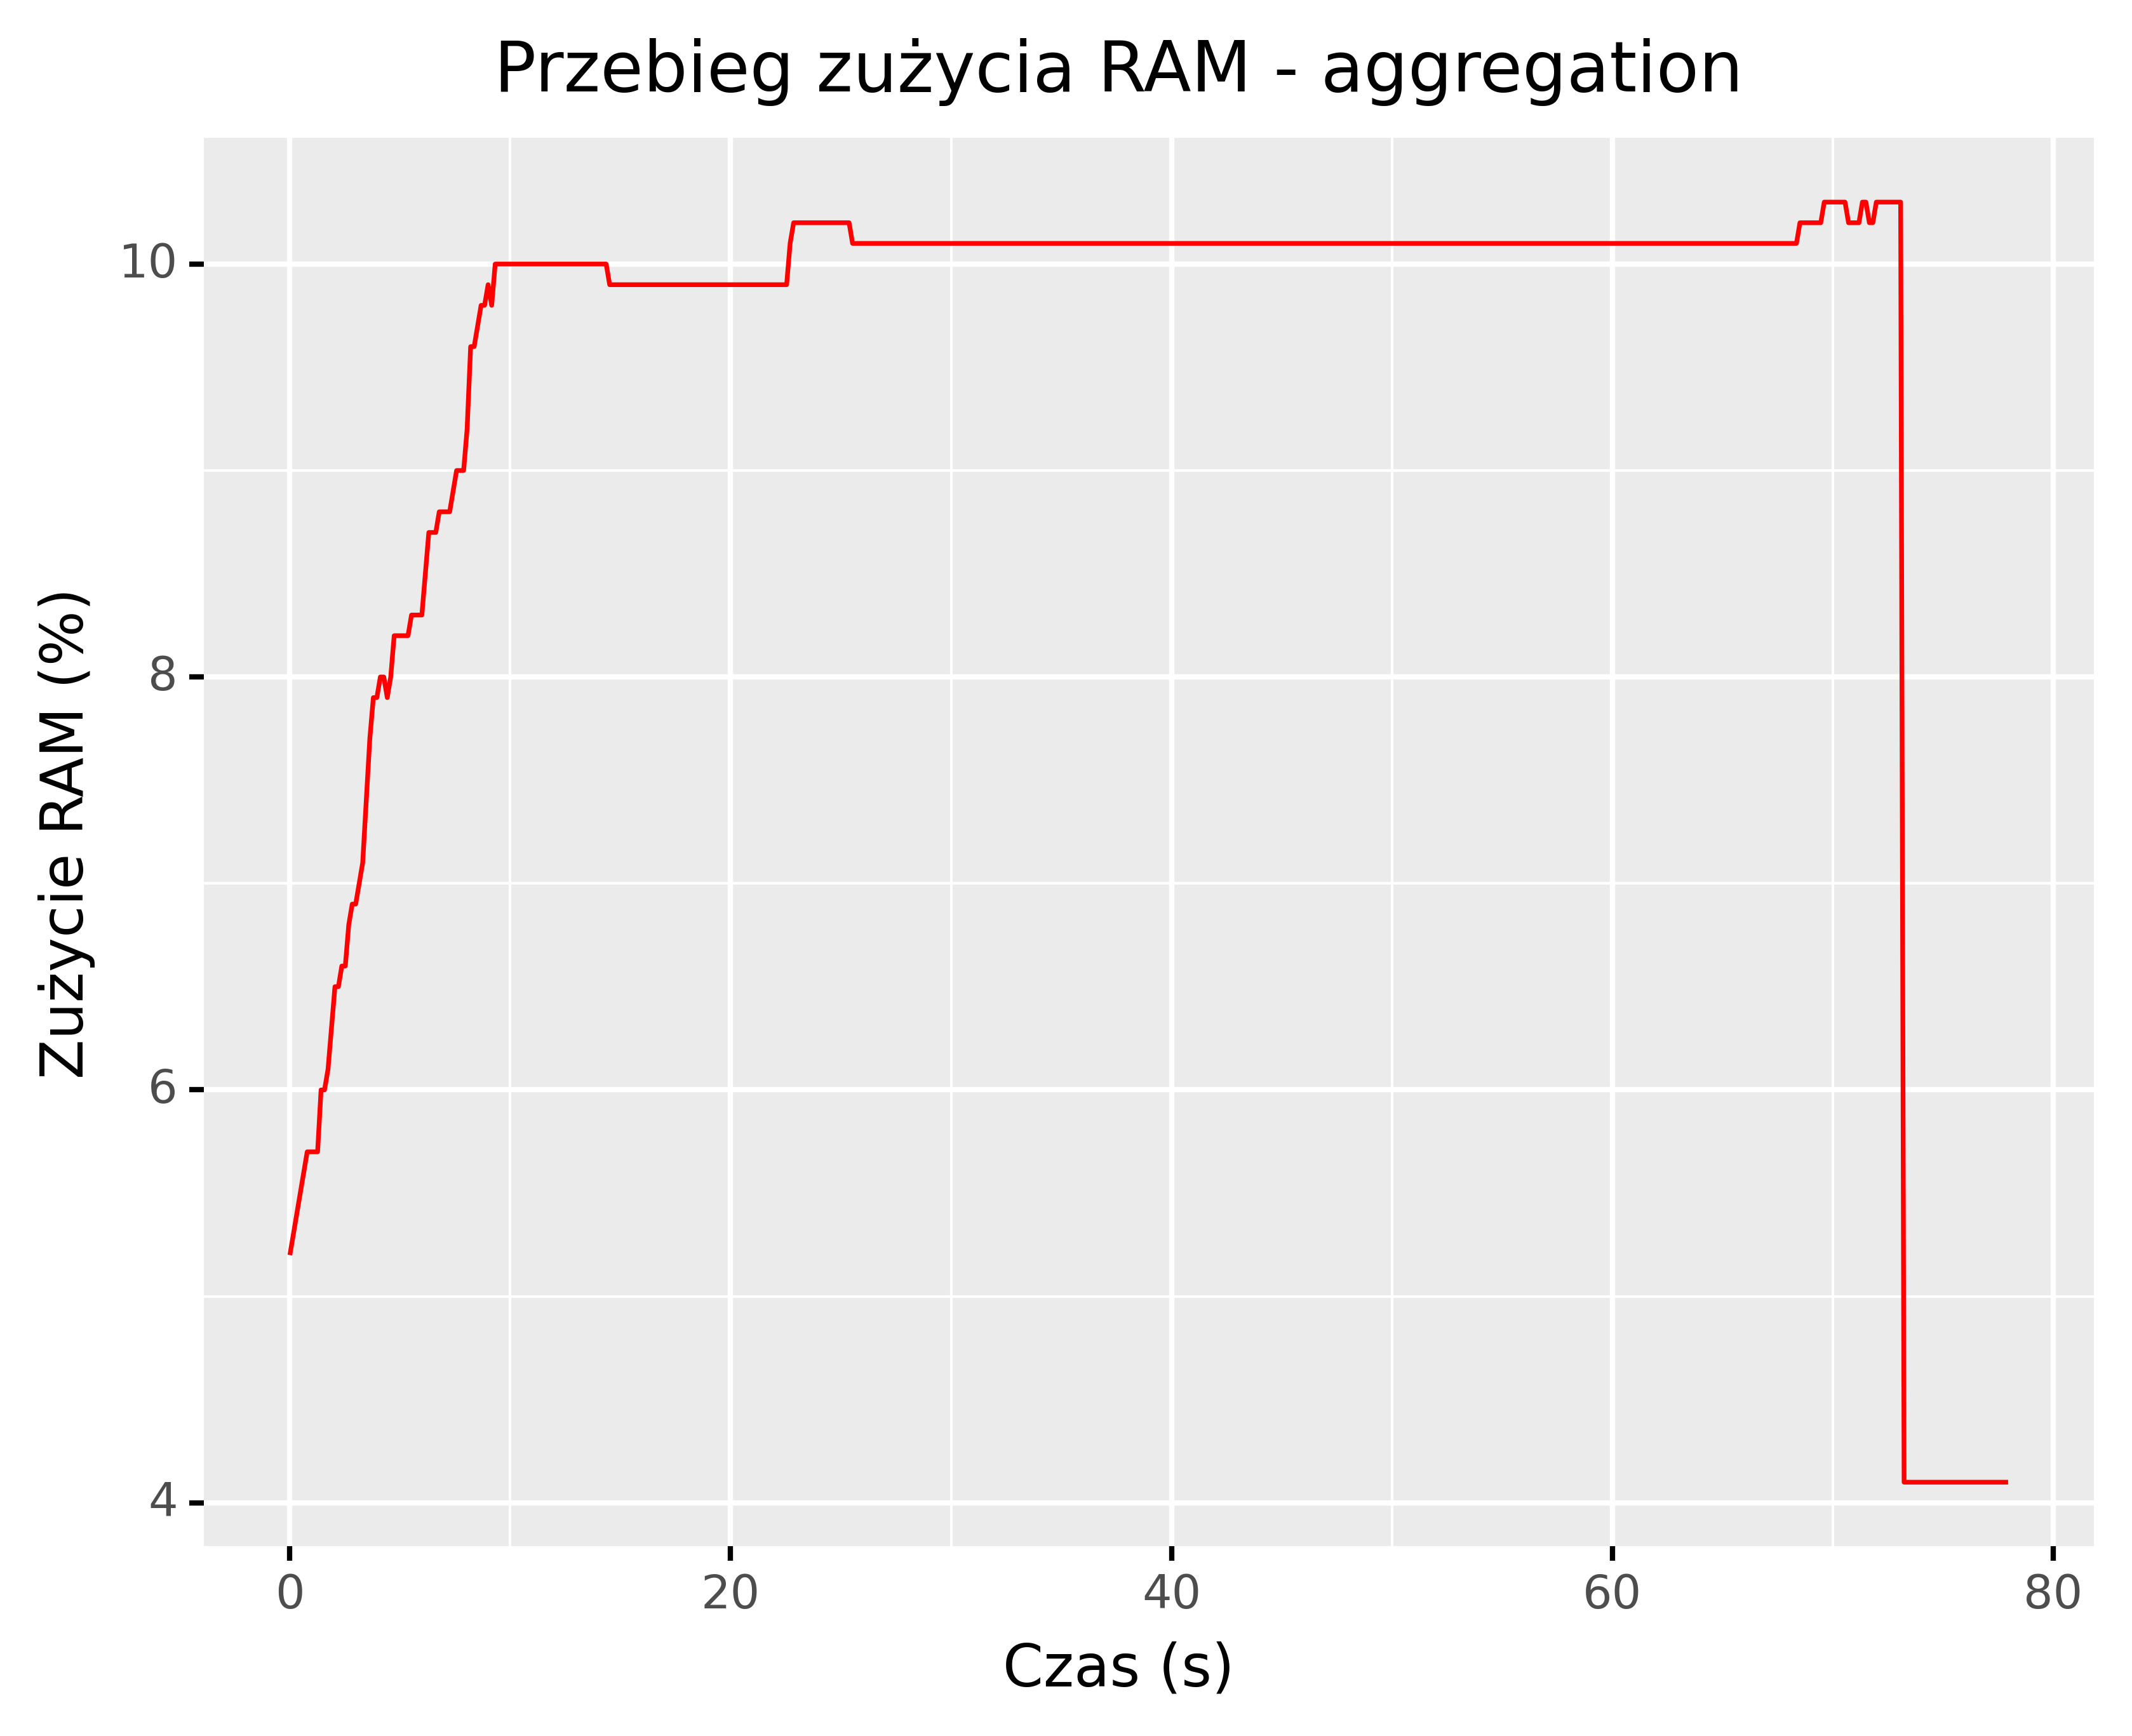
\includegraphics[width=0.5\textwidth]{figures/04-opis-danych/aggregation_example_ram_snapshot_1.png}\label{aggregation_example:f2}}
  \caption{Przykładowy przebieg zużycia zasobów dla agregacji (snapshot = 1)}
  \label{aggregation_example}
\end{figure}

\begin{figure}[H]
  \centering
  \subfloat[CPU]{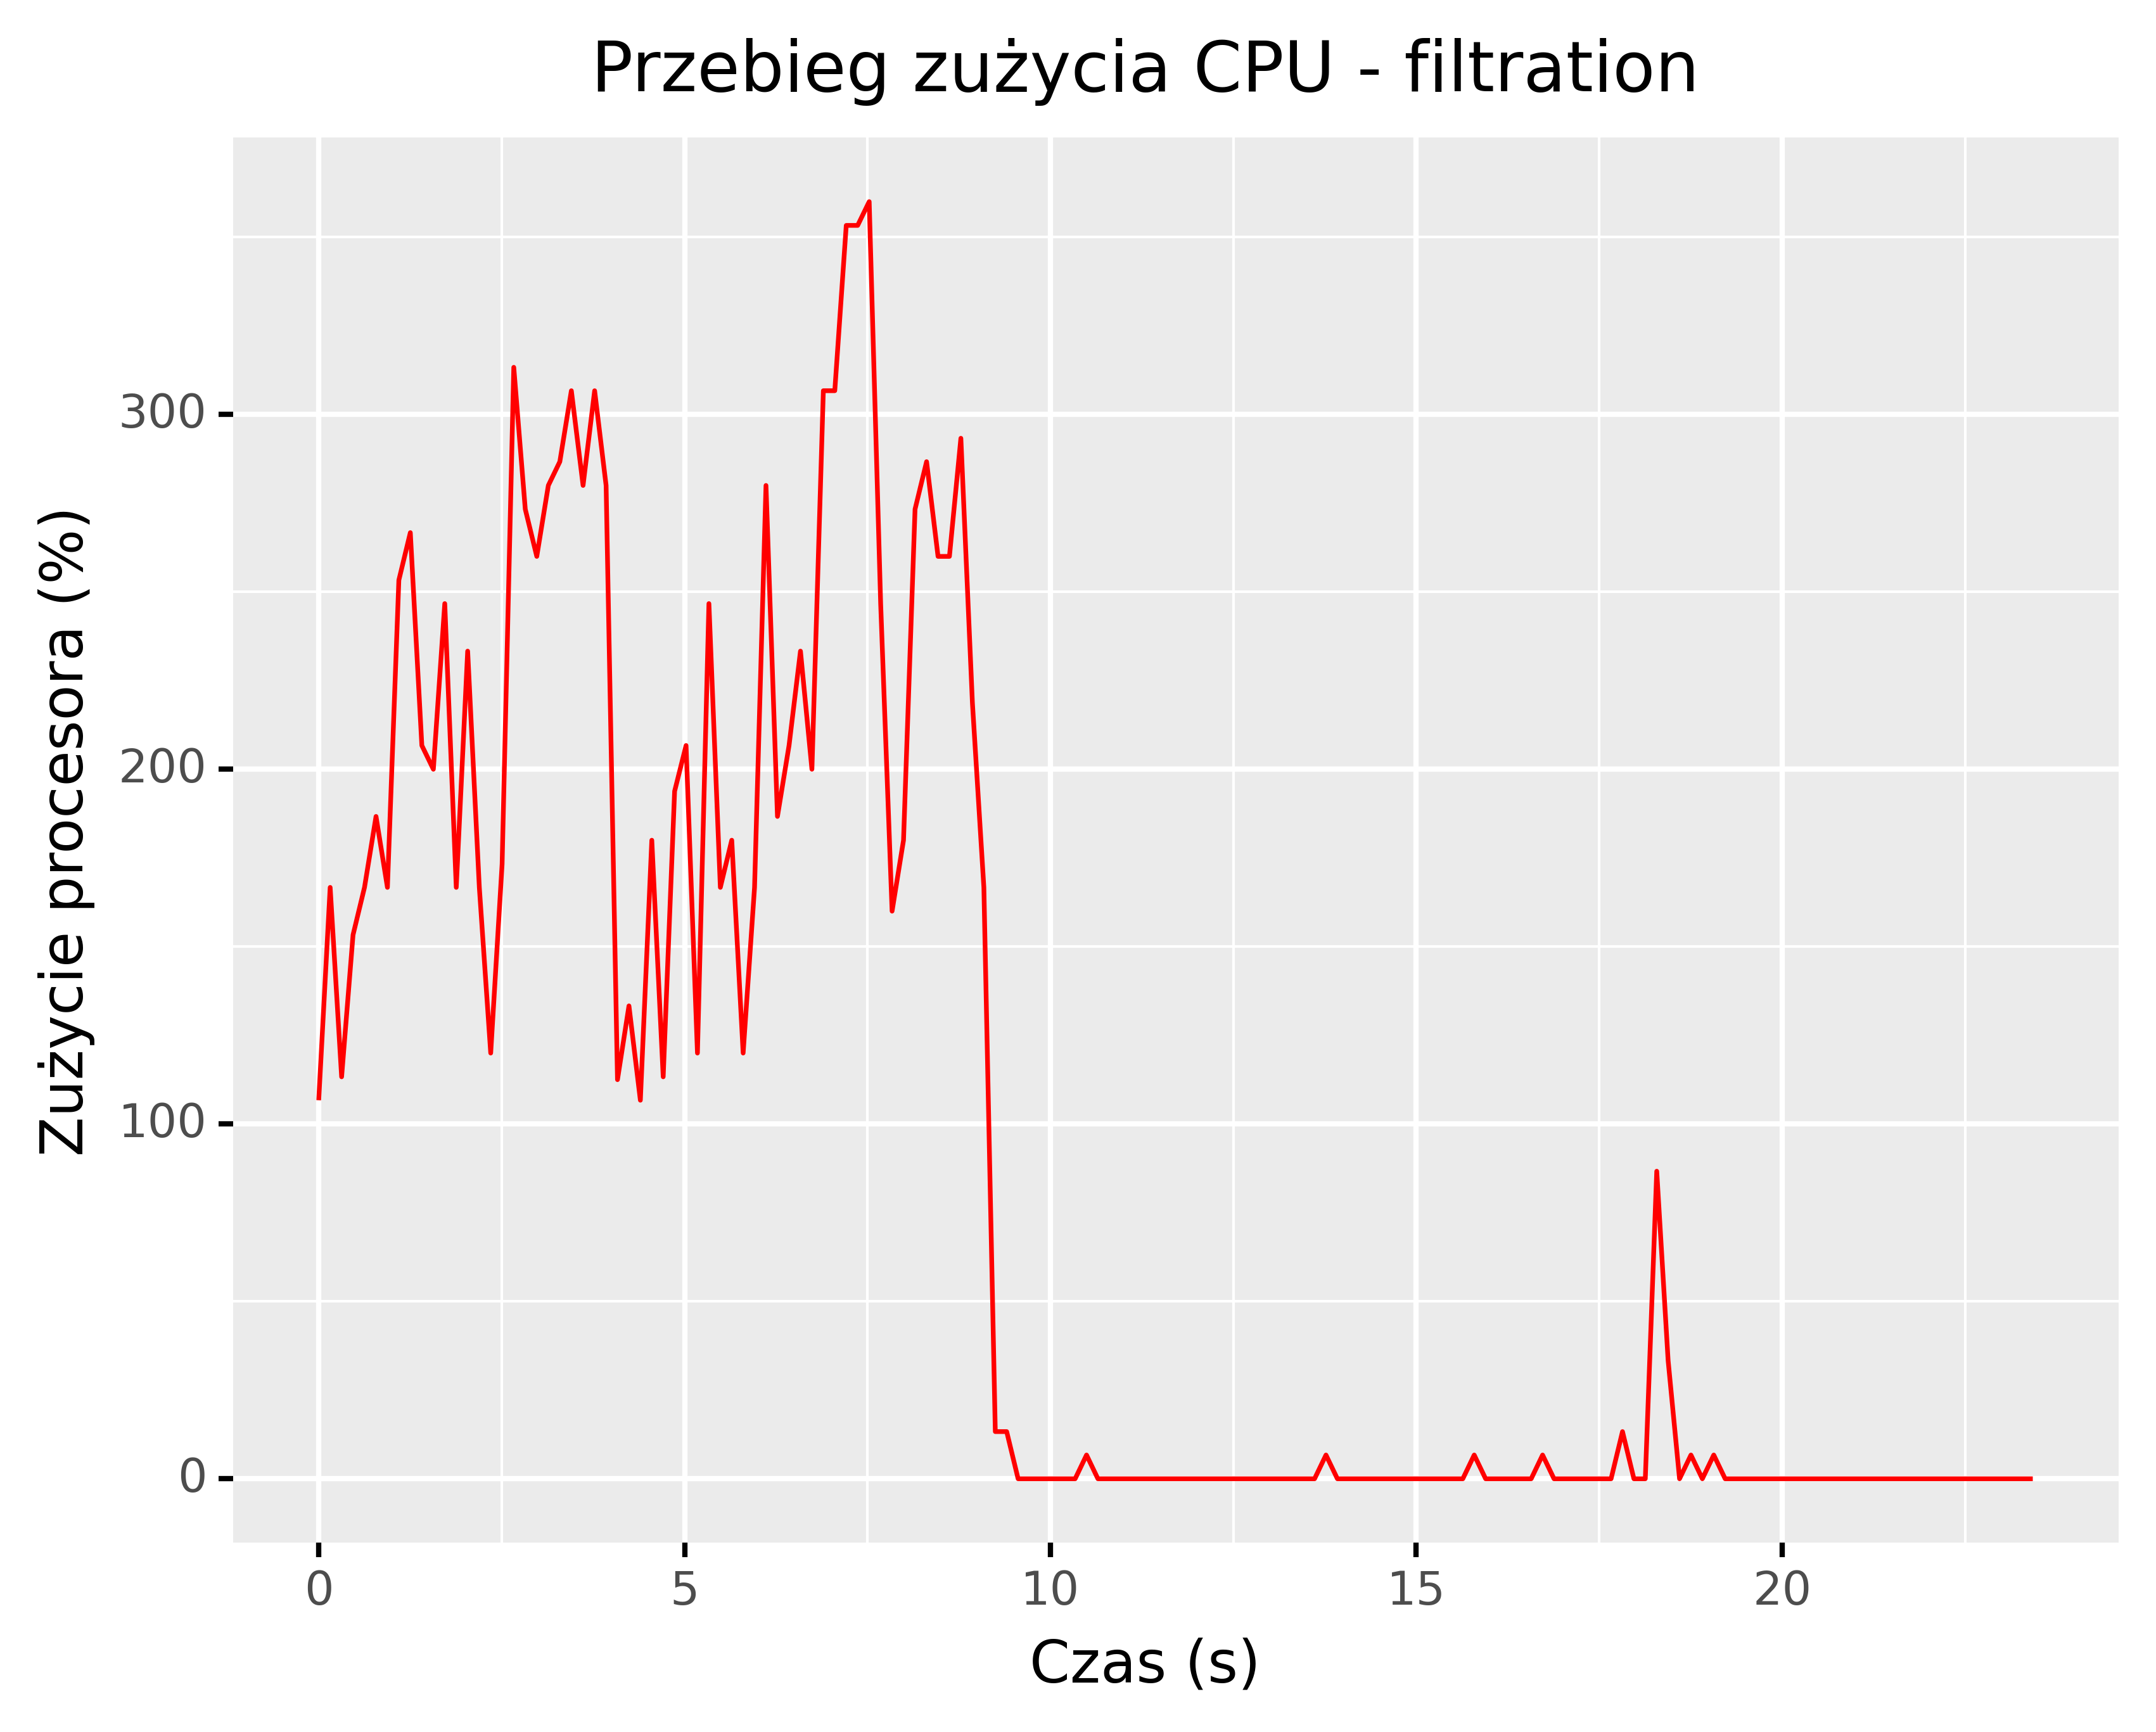
\includegraphics[width=0.5\textwidth]{figures/04-opis-danych/filtration_example_cpu_snapshot_1.png}\label{filtration:f1}}
  \hfill
  \subfloat[RAM]{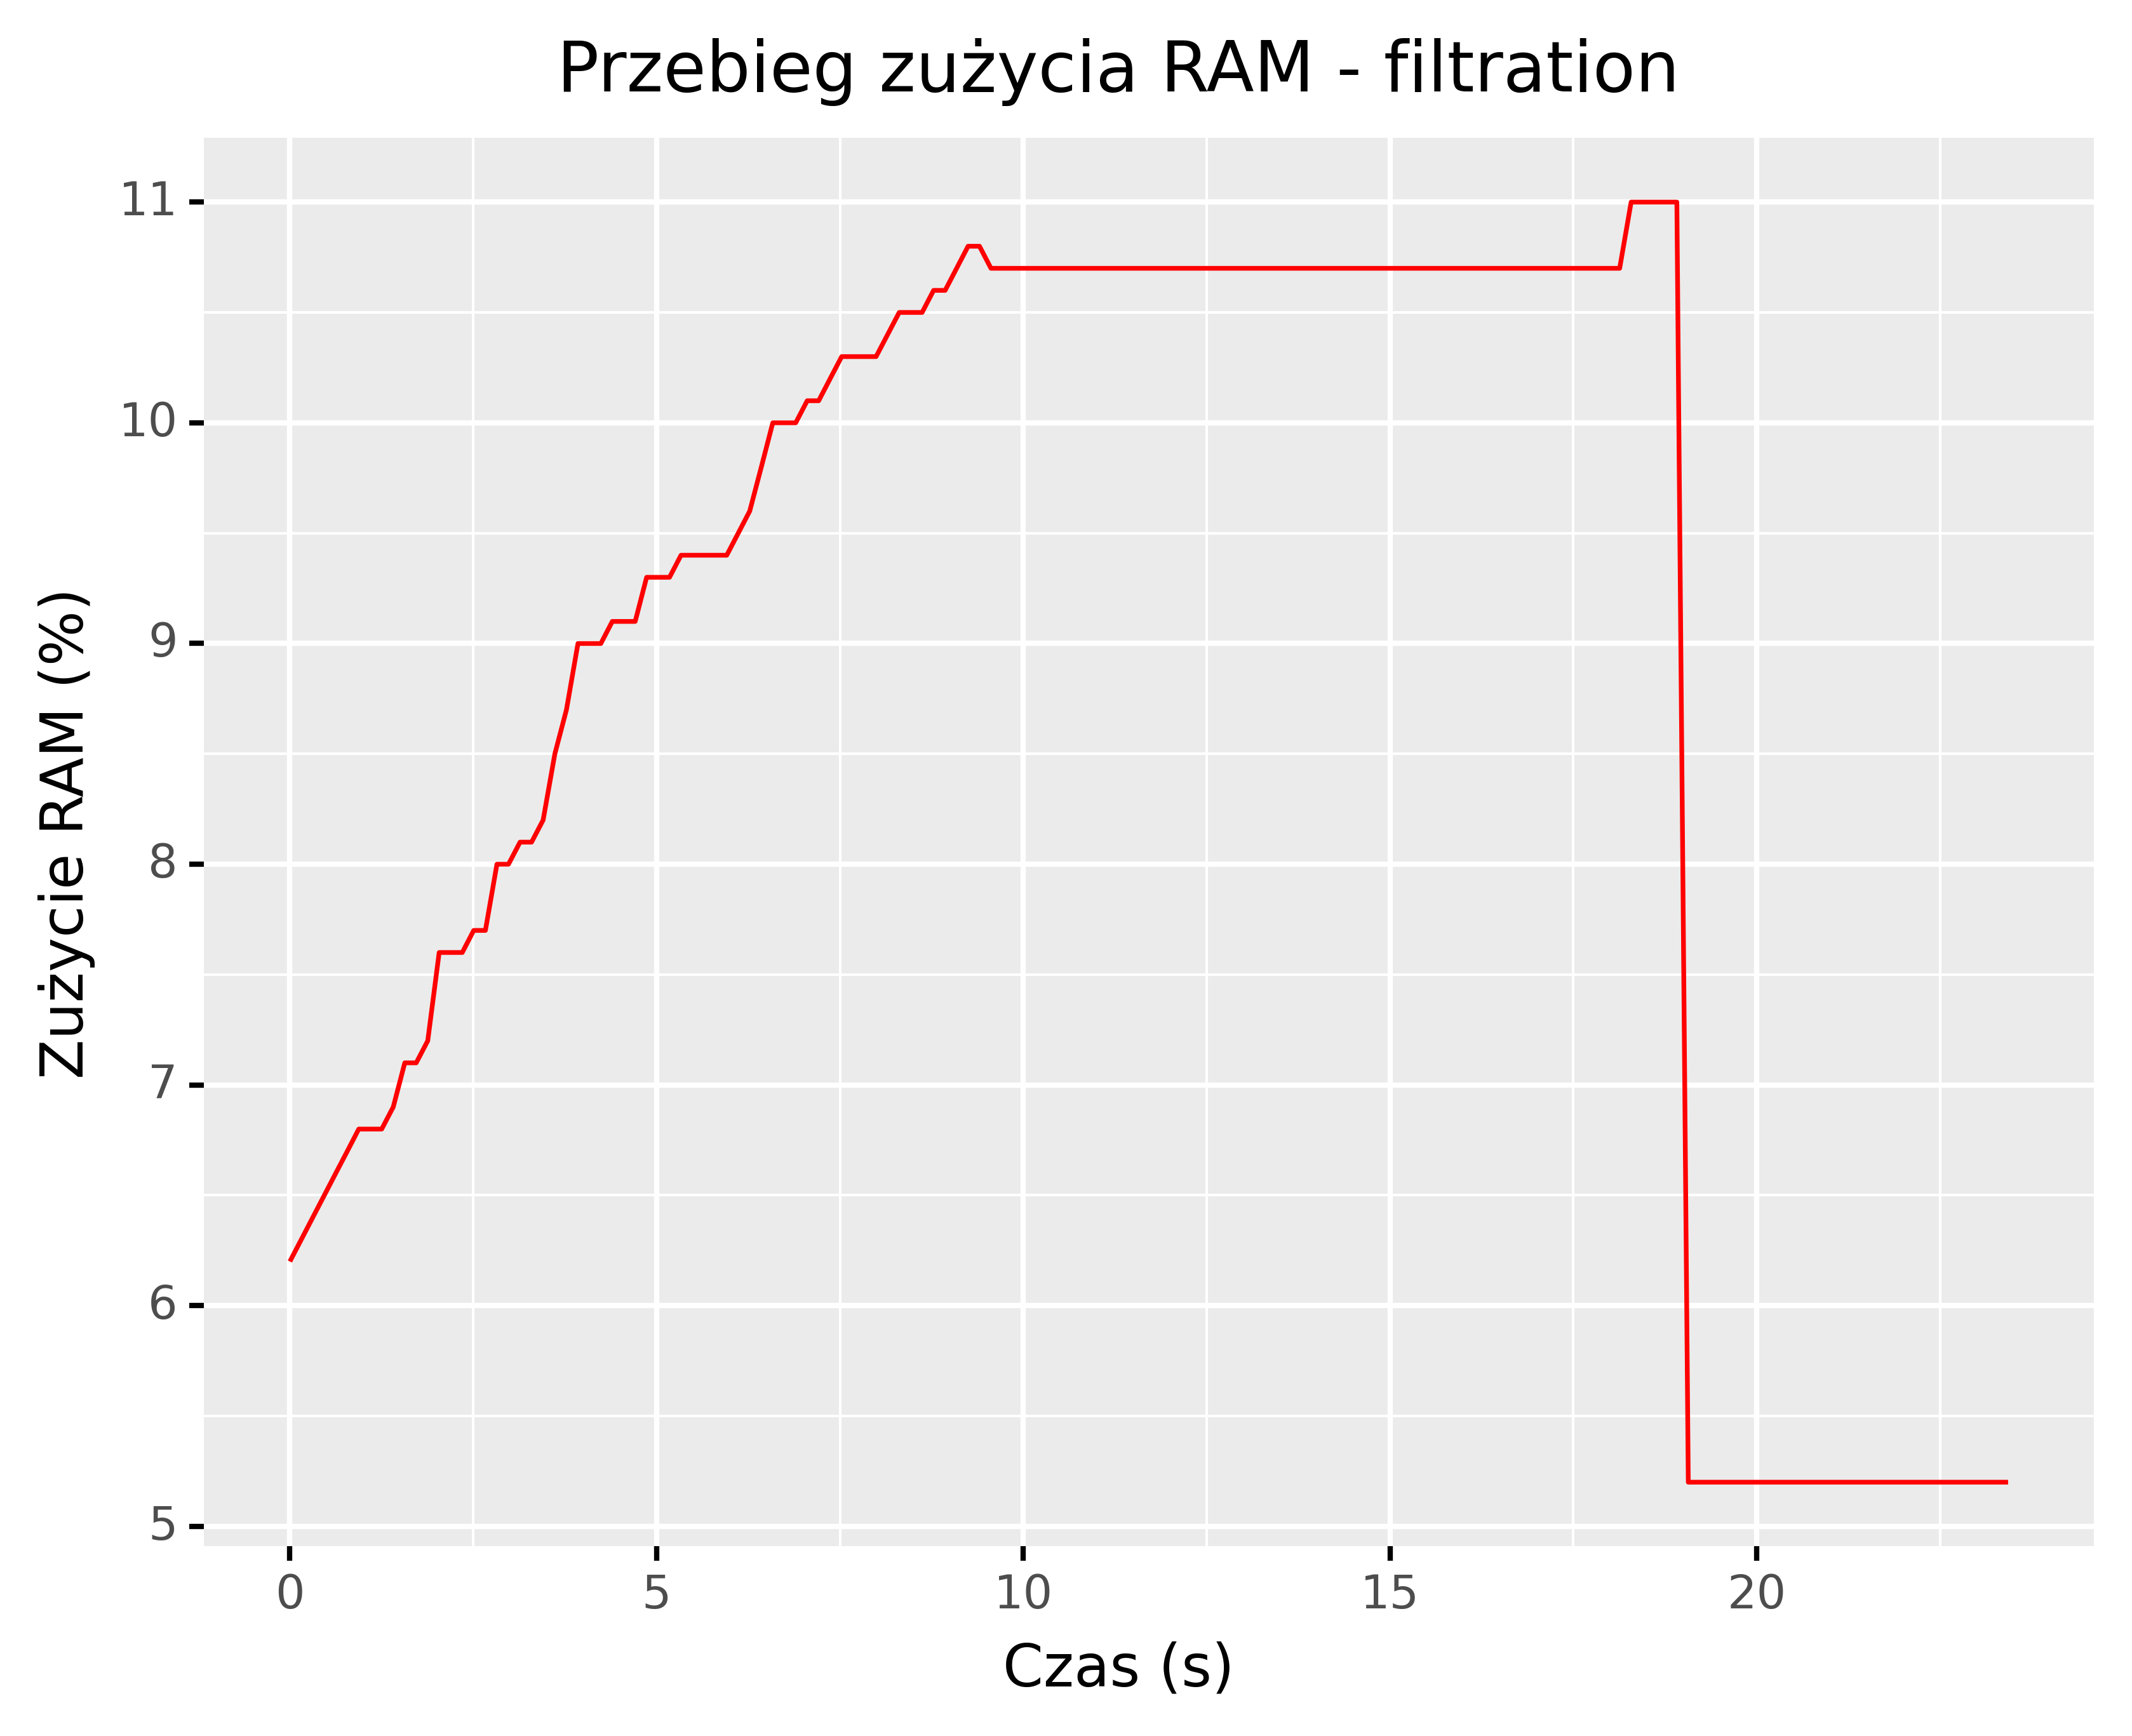
\includegraphics[width=0.5\textwidth]{figures/04-opis-danych/filtration_example_ram_snapshot_1.png}\label{filtration:f2}}
  \caption{Przykładowy przebieg zużycia zasobów dla filtracji (snapshot = 1)}
  \label{filtration_example}
\end{figure}

\begin{figure}[H]
  \centering
  \subfloat[CPU]{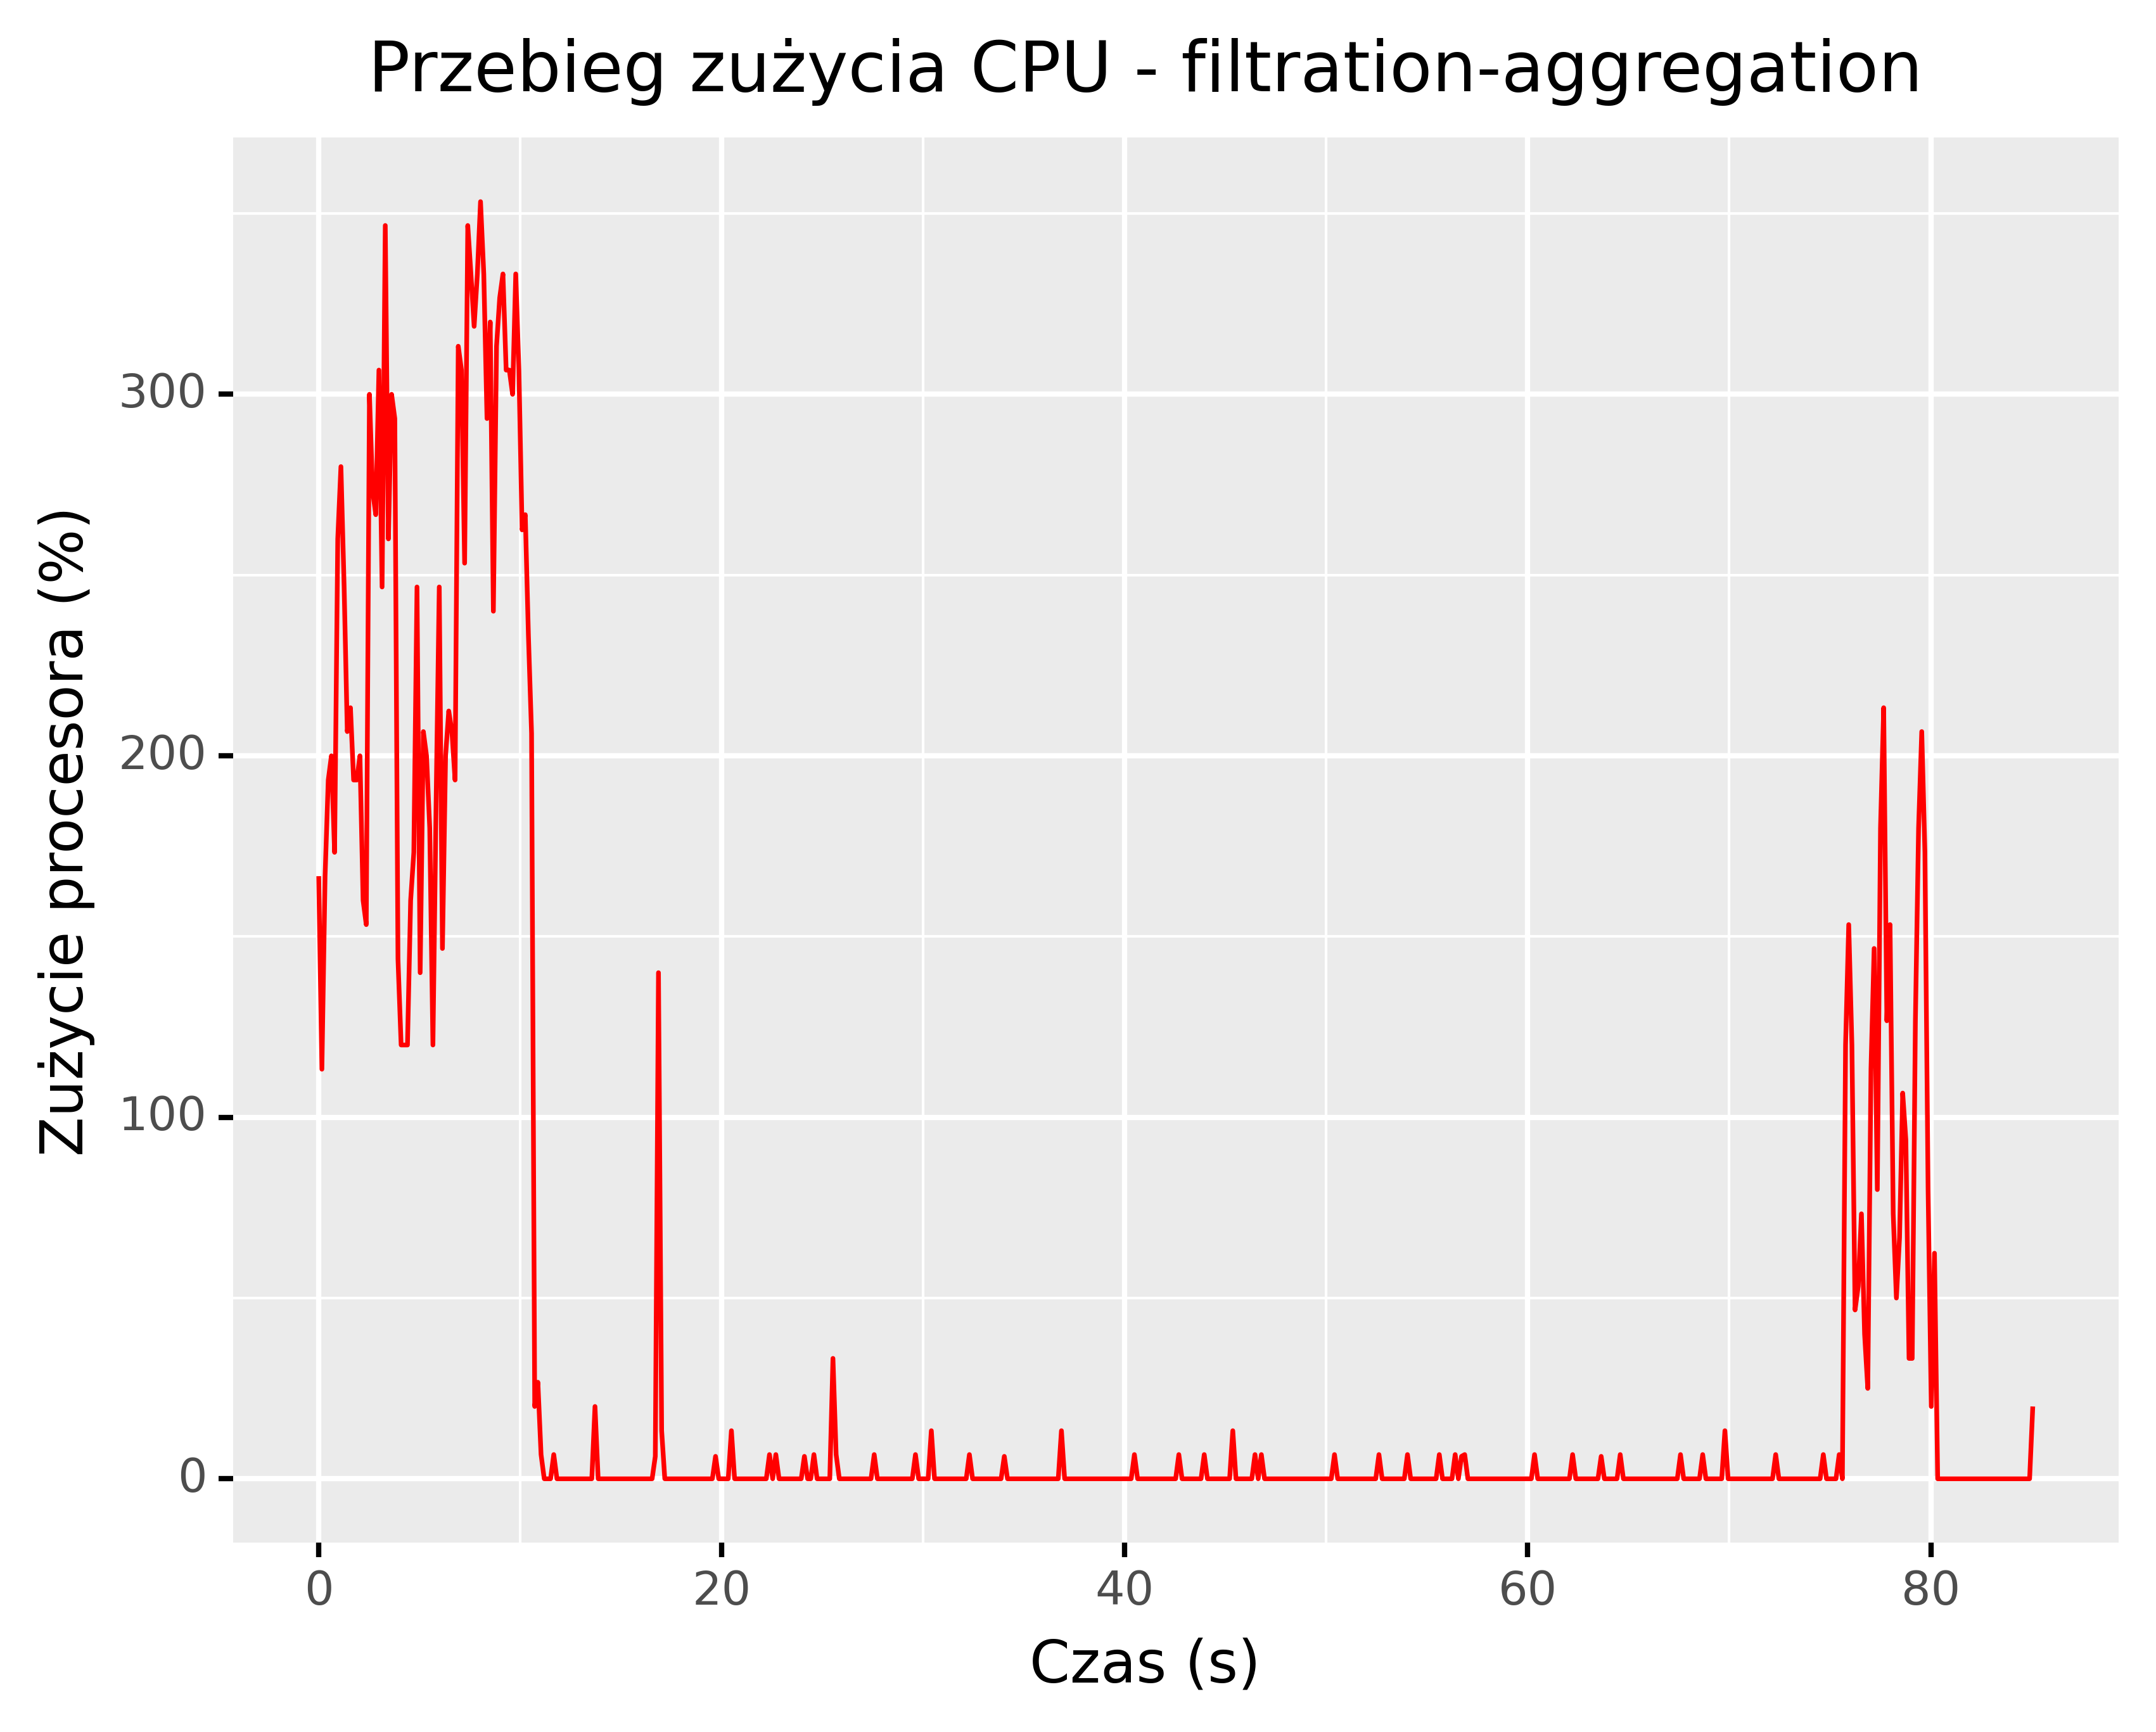
\includegraphics[width=0.5\textwidth]{figures/04-opis-danych/filtration-aggregation_example_cpu_snapshot_1.png}\label{filtration-aggregation:f1}}
  \hfill
  \subfloat[RAM]{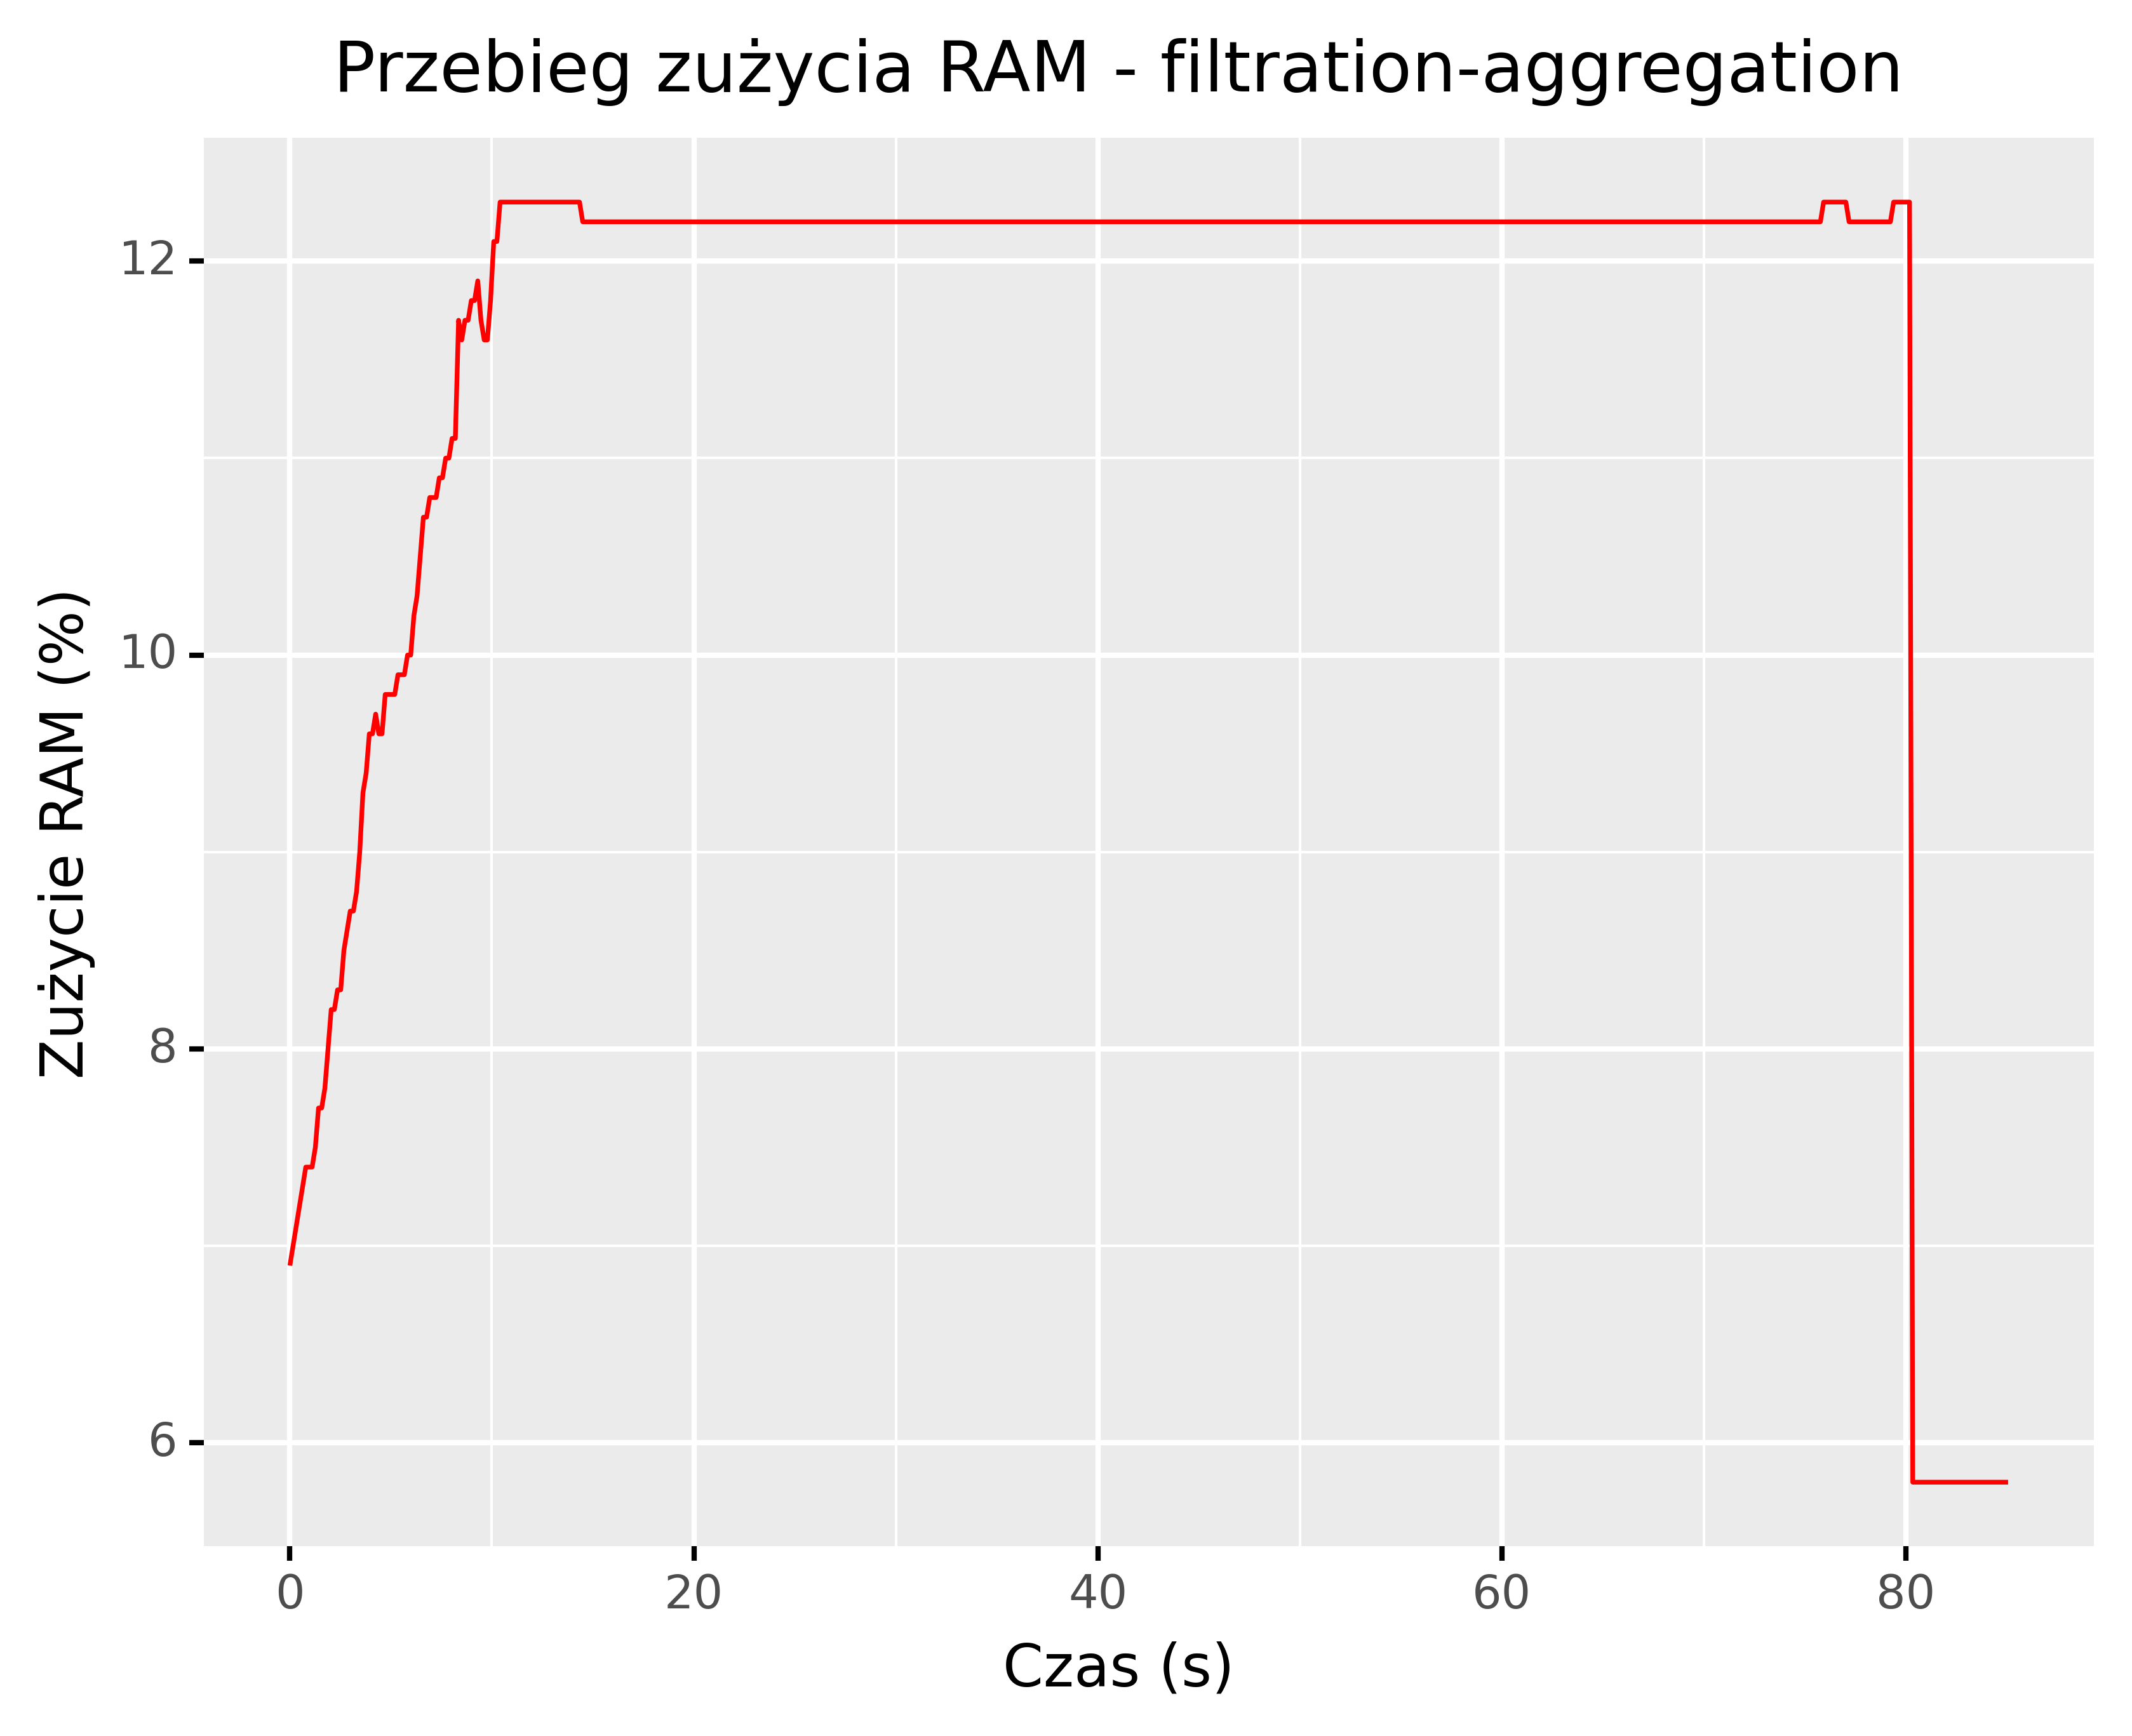
\includegraphics[width=0.5\textwidth]{figures/04-opis-danych/filtration-aggregation_example_ram_snapshot_1.png}\label{filtration-aggregation:f2}}
  \caption{Przykładowy przebieg zużycia zasobów dla filtracjo-agregacji (snapshot = 1)}
  \label{filtration-aggregation_example}
\end{figure}

\begin{figure}[H]
  \centering
  \subfloat[CPU]{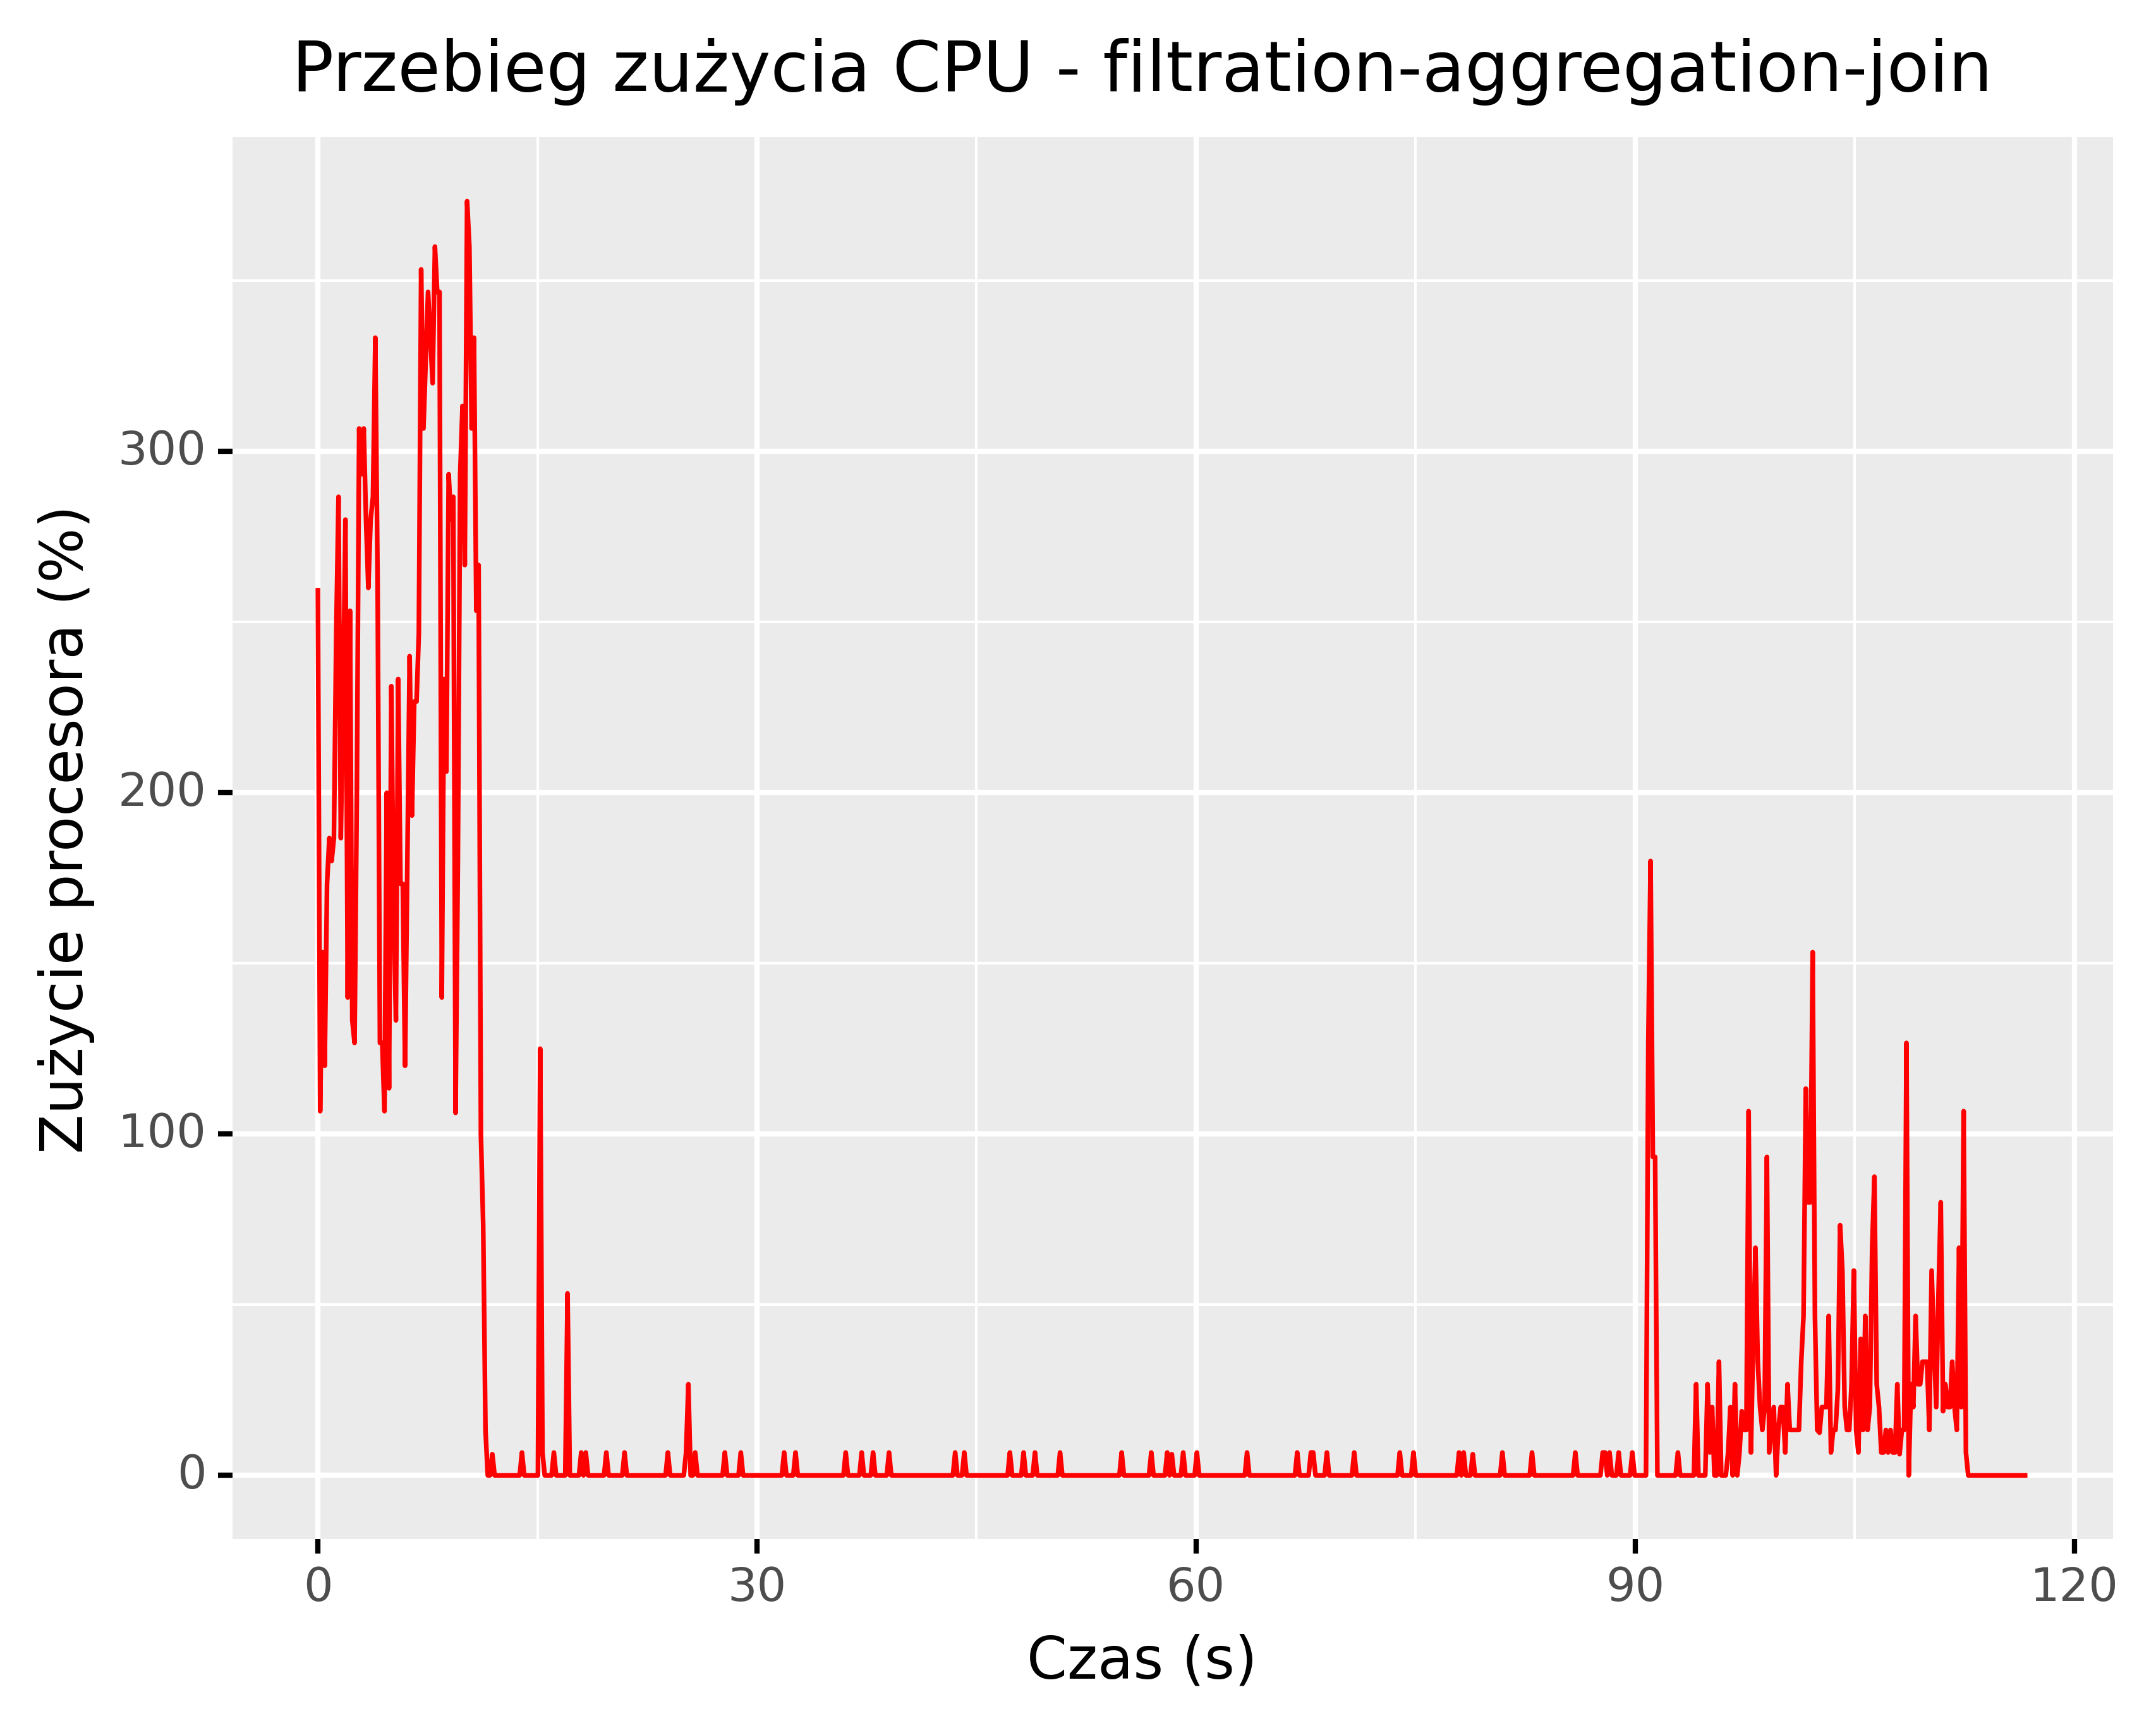
\includegraphics[width=0.5\textwidth]{figures/04-opis-danych/filtration-aggregation-join_example_cpu_snapshot_1.png}\label{filtration-aggregation-join:f1}}
  \hfill
  \subfloat[RAM]{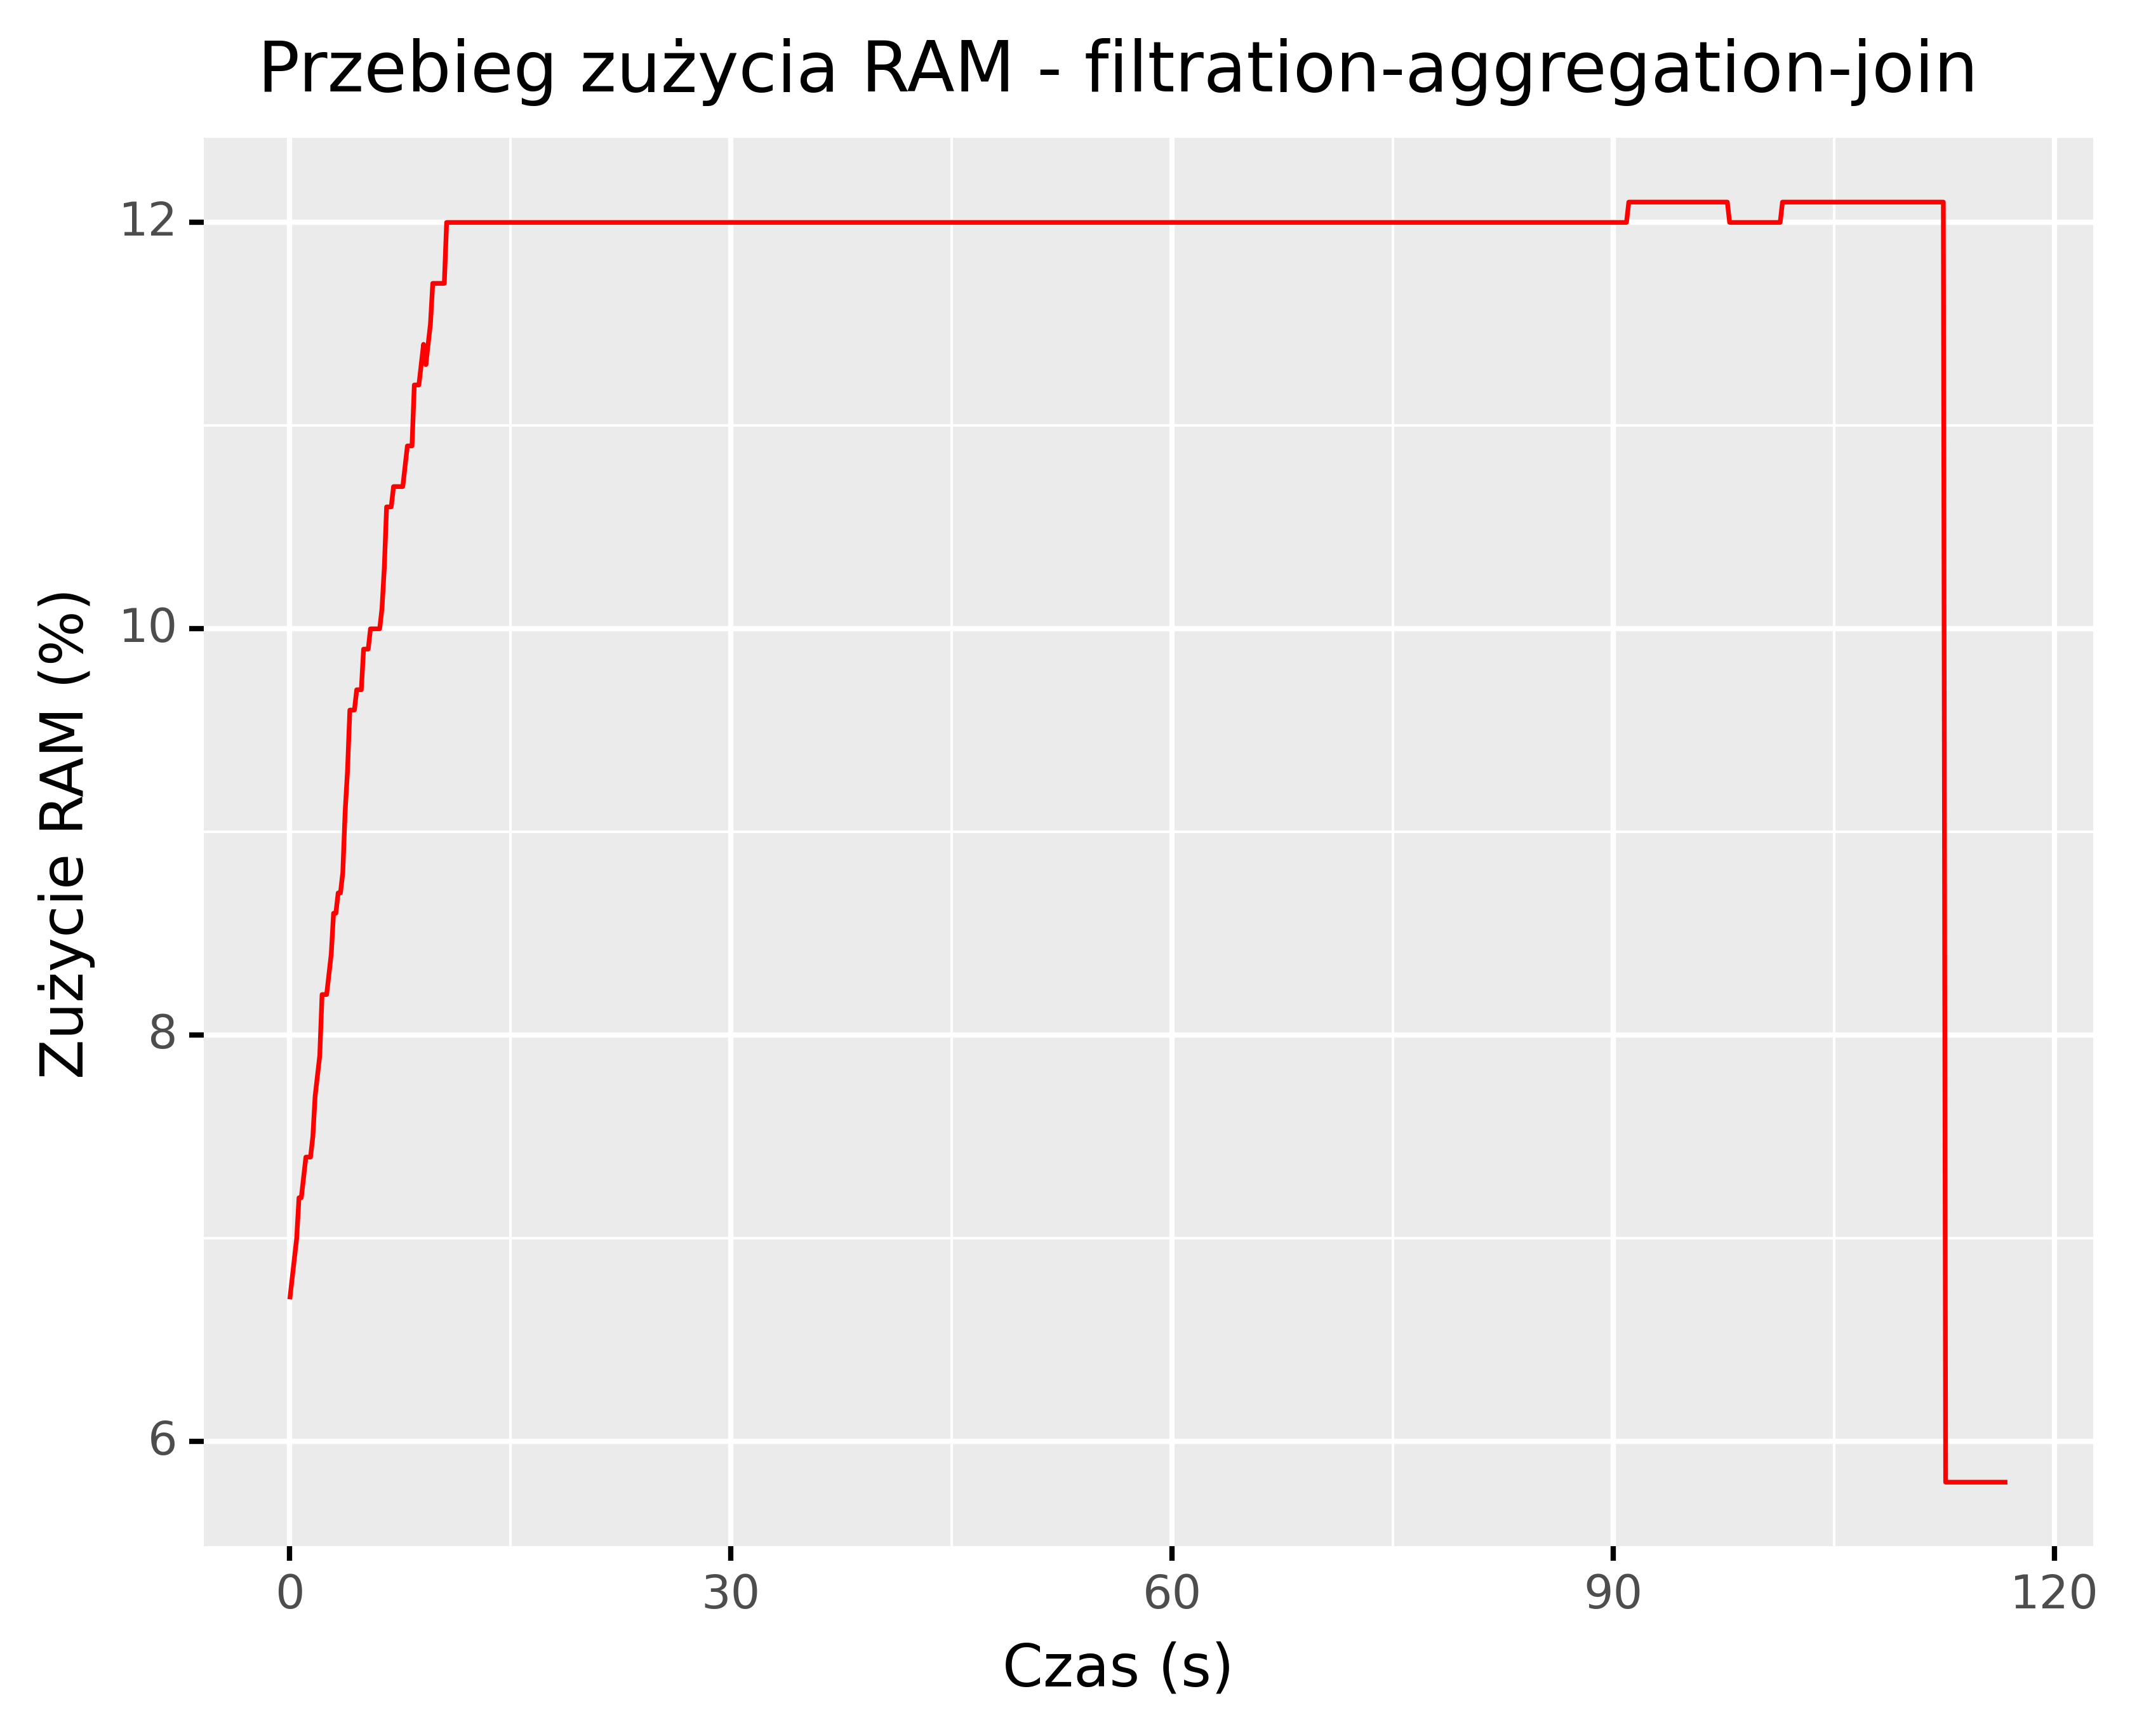
\includegraphics[width=0.5\textwidth]{figures/04-opis-danych/filtration-aggregation-join_example_ram_snapshot_1.png}\label{filtration-aggregation-join:f2}}
  \caption{Przykładowy przebieg zużycia zasobów dla filtracjo-agregacji z połączeniem (snapshot = 1)}
  \label{filtration-aggregation-join_example}
\end{figure}

\begin{figure}[!h]
  \centering
  \subfloat[CPU]{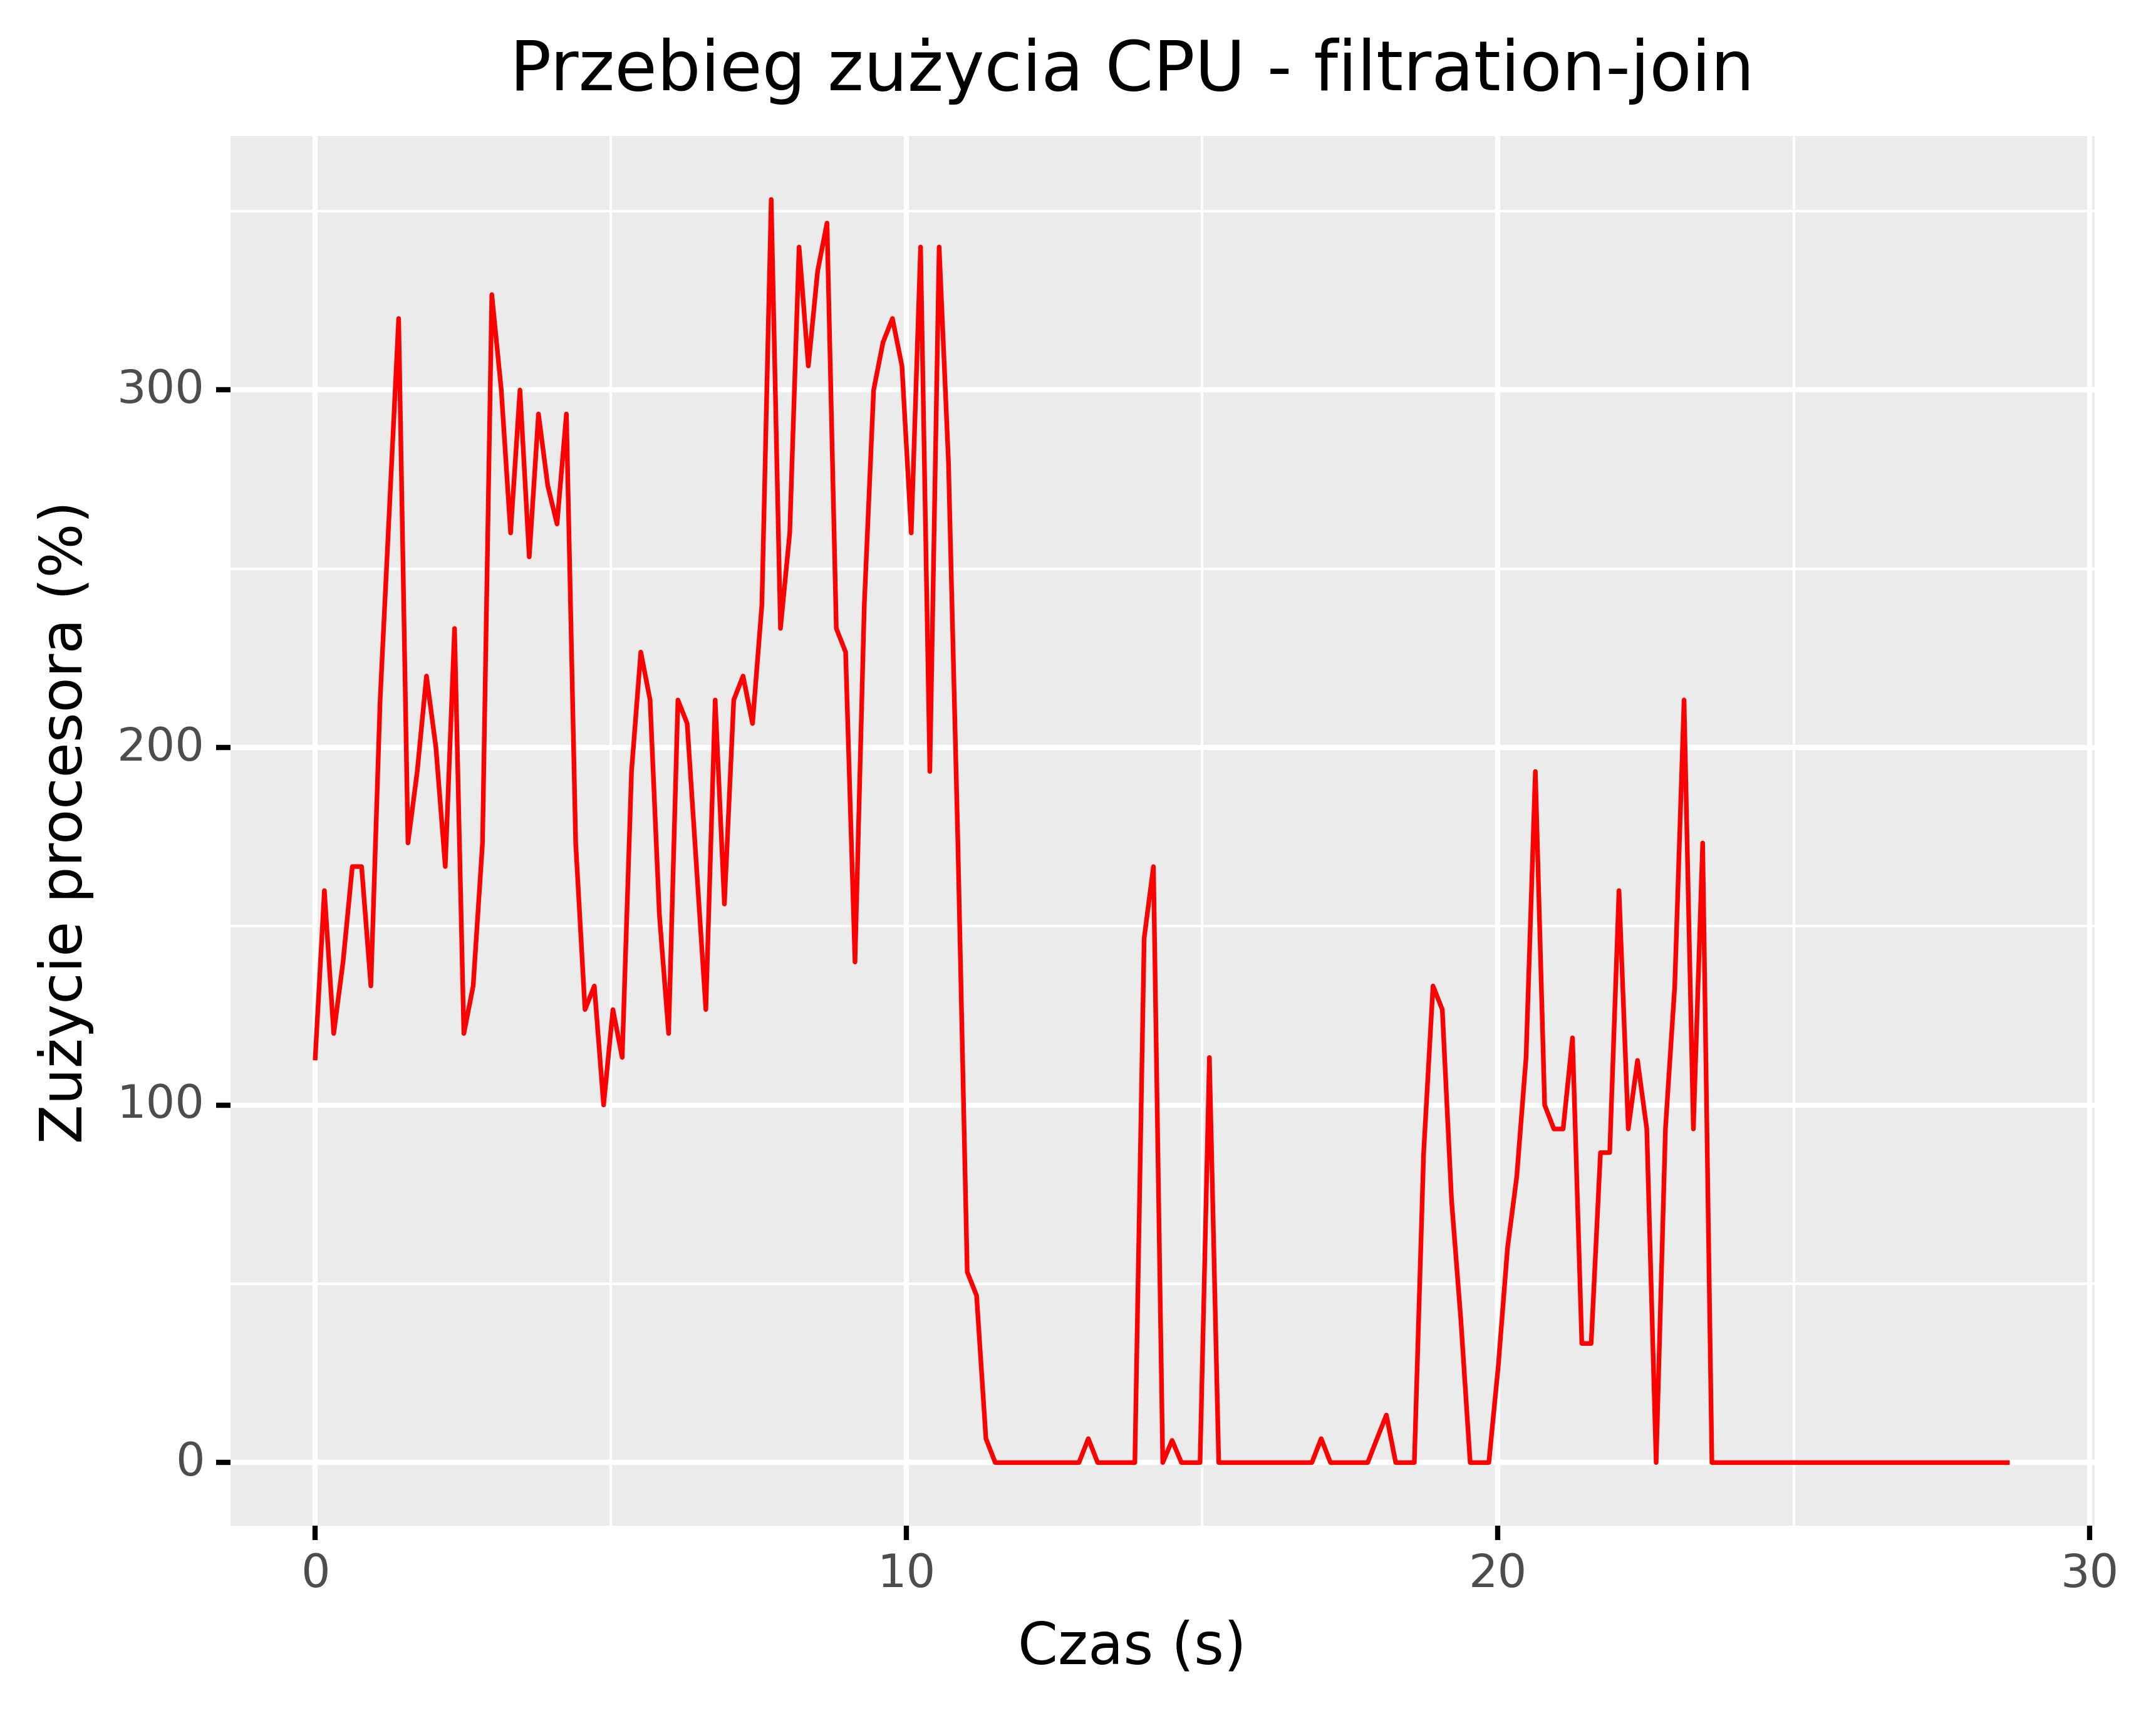
\includegraphics[width=0.5\textwidth]{figures/04-opis-danych/filtration-join_example_cpu_snapshot_1.png}\label{filtration-join_example:f1}}
  \hfill
  \subfloat[RAM]{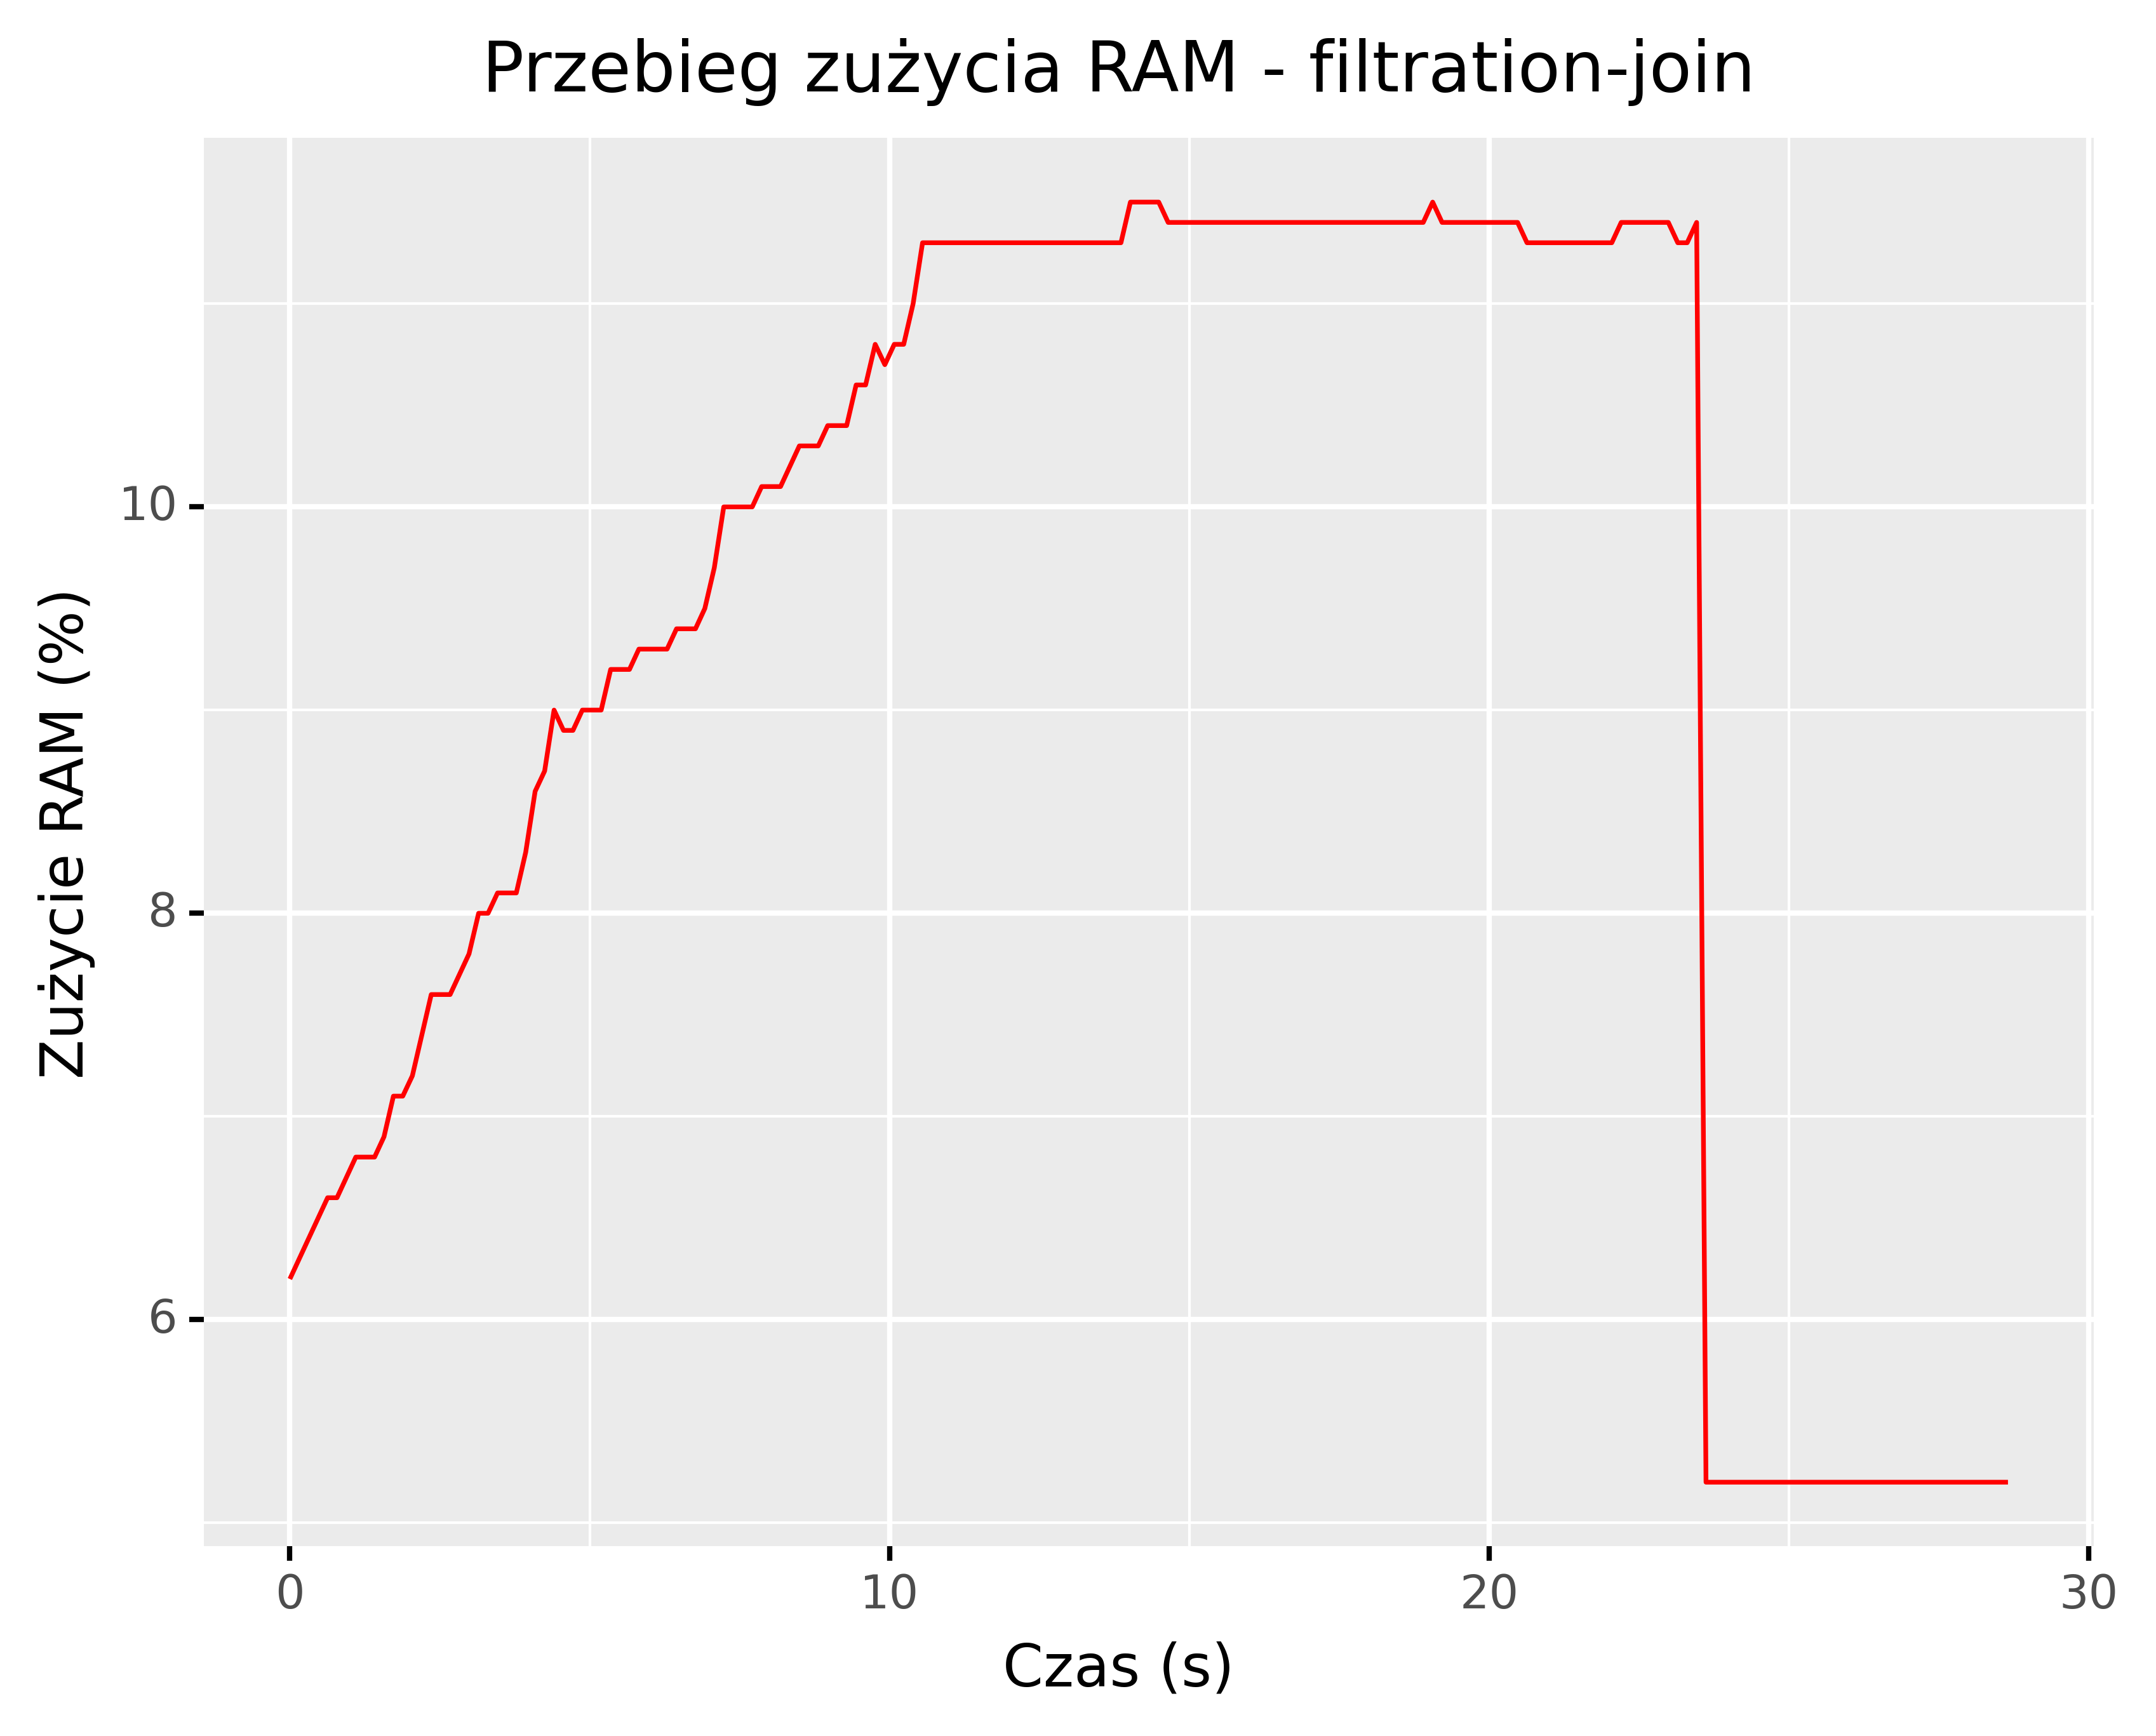
\includegraphics[width=0.5\textwidth]{figures/04-opis-danych/filtration-join_example_ram_snapshot_1.png}\label{filtration-join_example:f2}}
  \caption{Przykładowy przebieg zużycia zasobów dla filtracji z połączeniem (snapshot = 1)}
  \label{filtration-join_example}
  
\end{figure}

Na rysunkach \ref{aggregation_example} do \ref{filtration-join_example} widać, że wykresy CPU są bardzo ostre i mogły by zyskać na wygładzeniu krawędzi. Wykonaliśmy to przy użyciu średniej w oknie przesuwnym. Okno brało pod uwagę liczbę próbek zależną od tego jak dużo okno czasowe chcemy brać pod uwagę. Próbki są zebrane w odstępach co 0.15 sekundy, więc ok. sześciu próbek równe jest jednej sekundzie. Poniżej znajdują się wykresy przestawiający wygląd wykresów po wygładzeniu dla różnej liczby próbek dla przykładowego przebiegu agregacji.

\begin{figure}[H]
  \centering
  \subfloat[CPU]{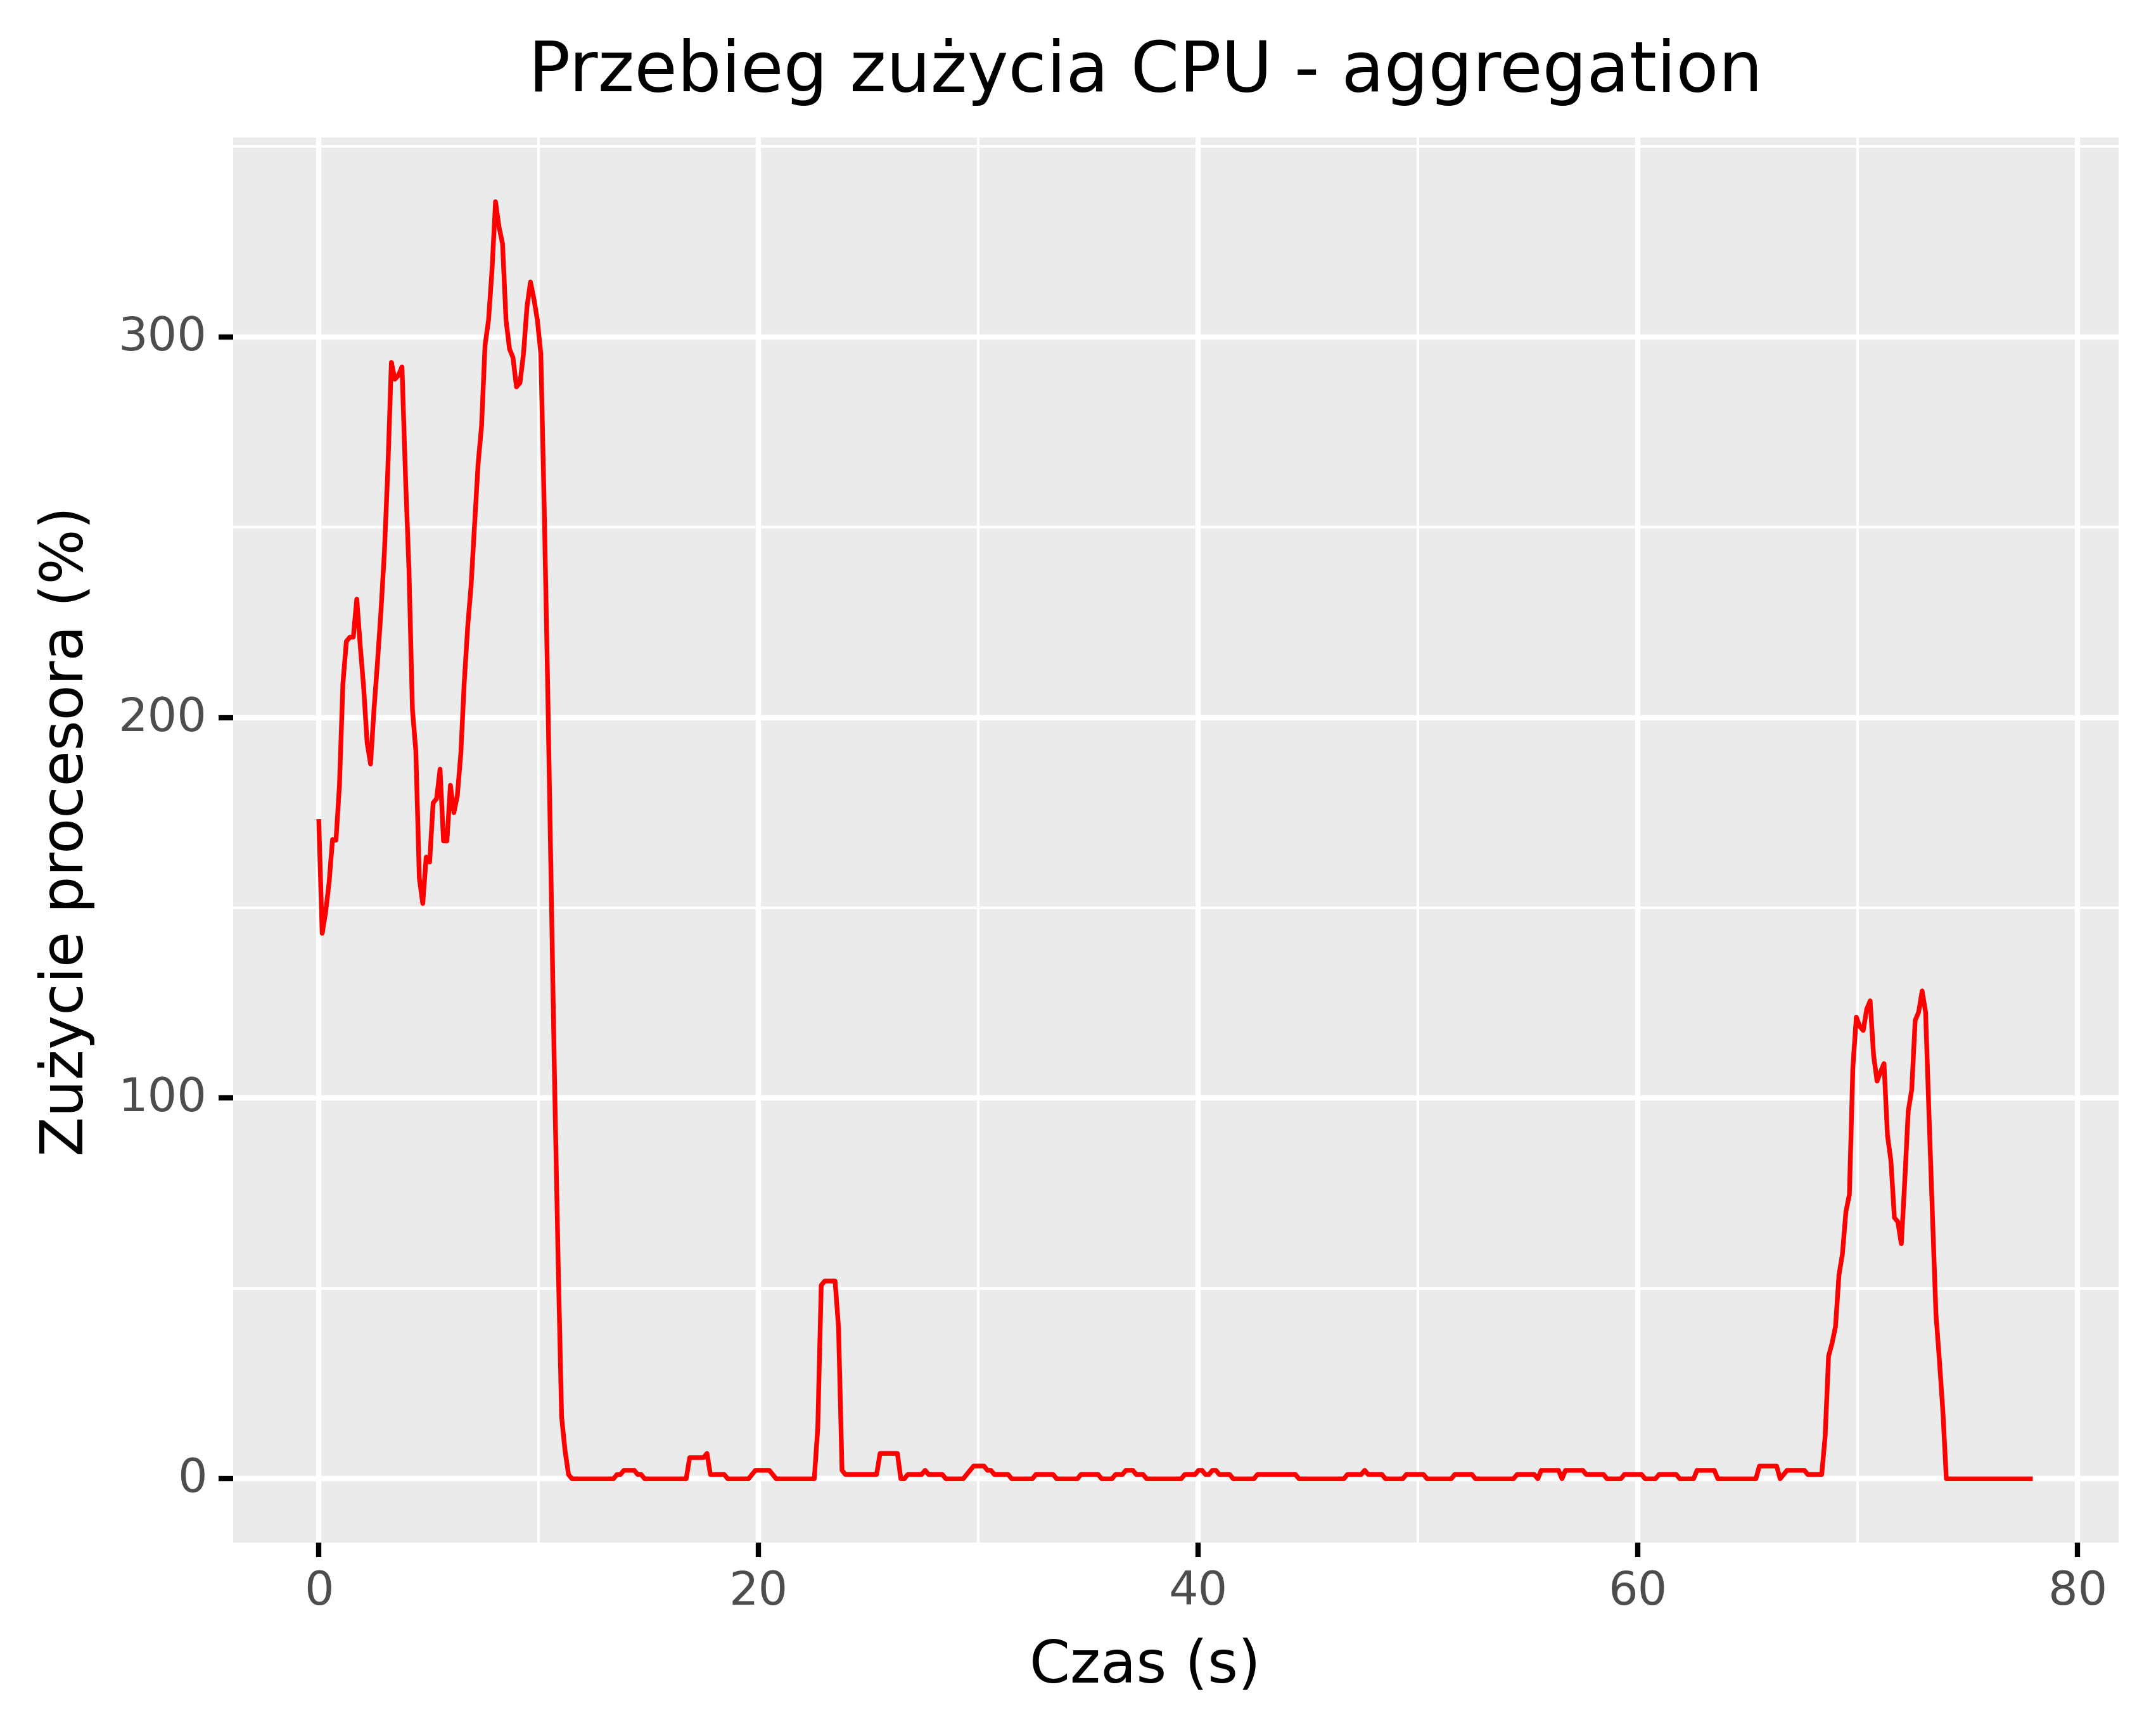
\includegraphics[width=0.5\textwidth]{figures/04-opis-danych/aggregation_smooth_6_cpu_snapshot_1.png}\label{aggregation_smooth_6:f1}}
  \hfill
  \subfloat[RAM]{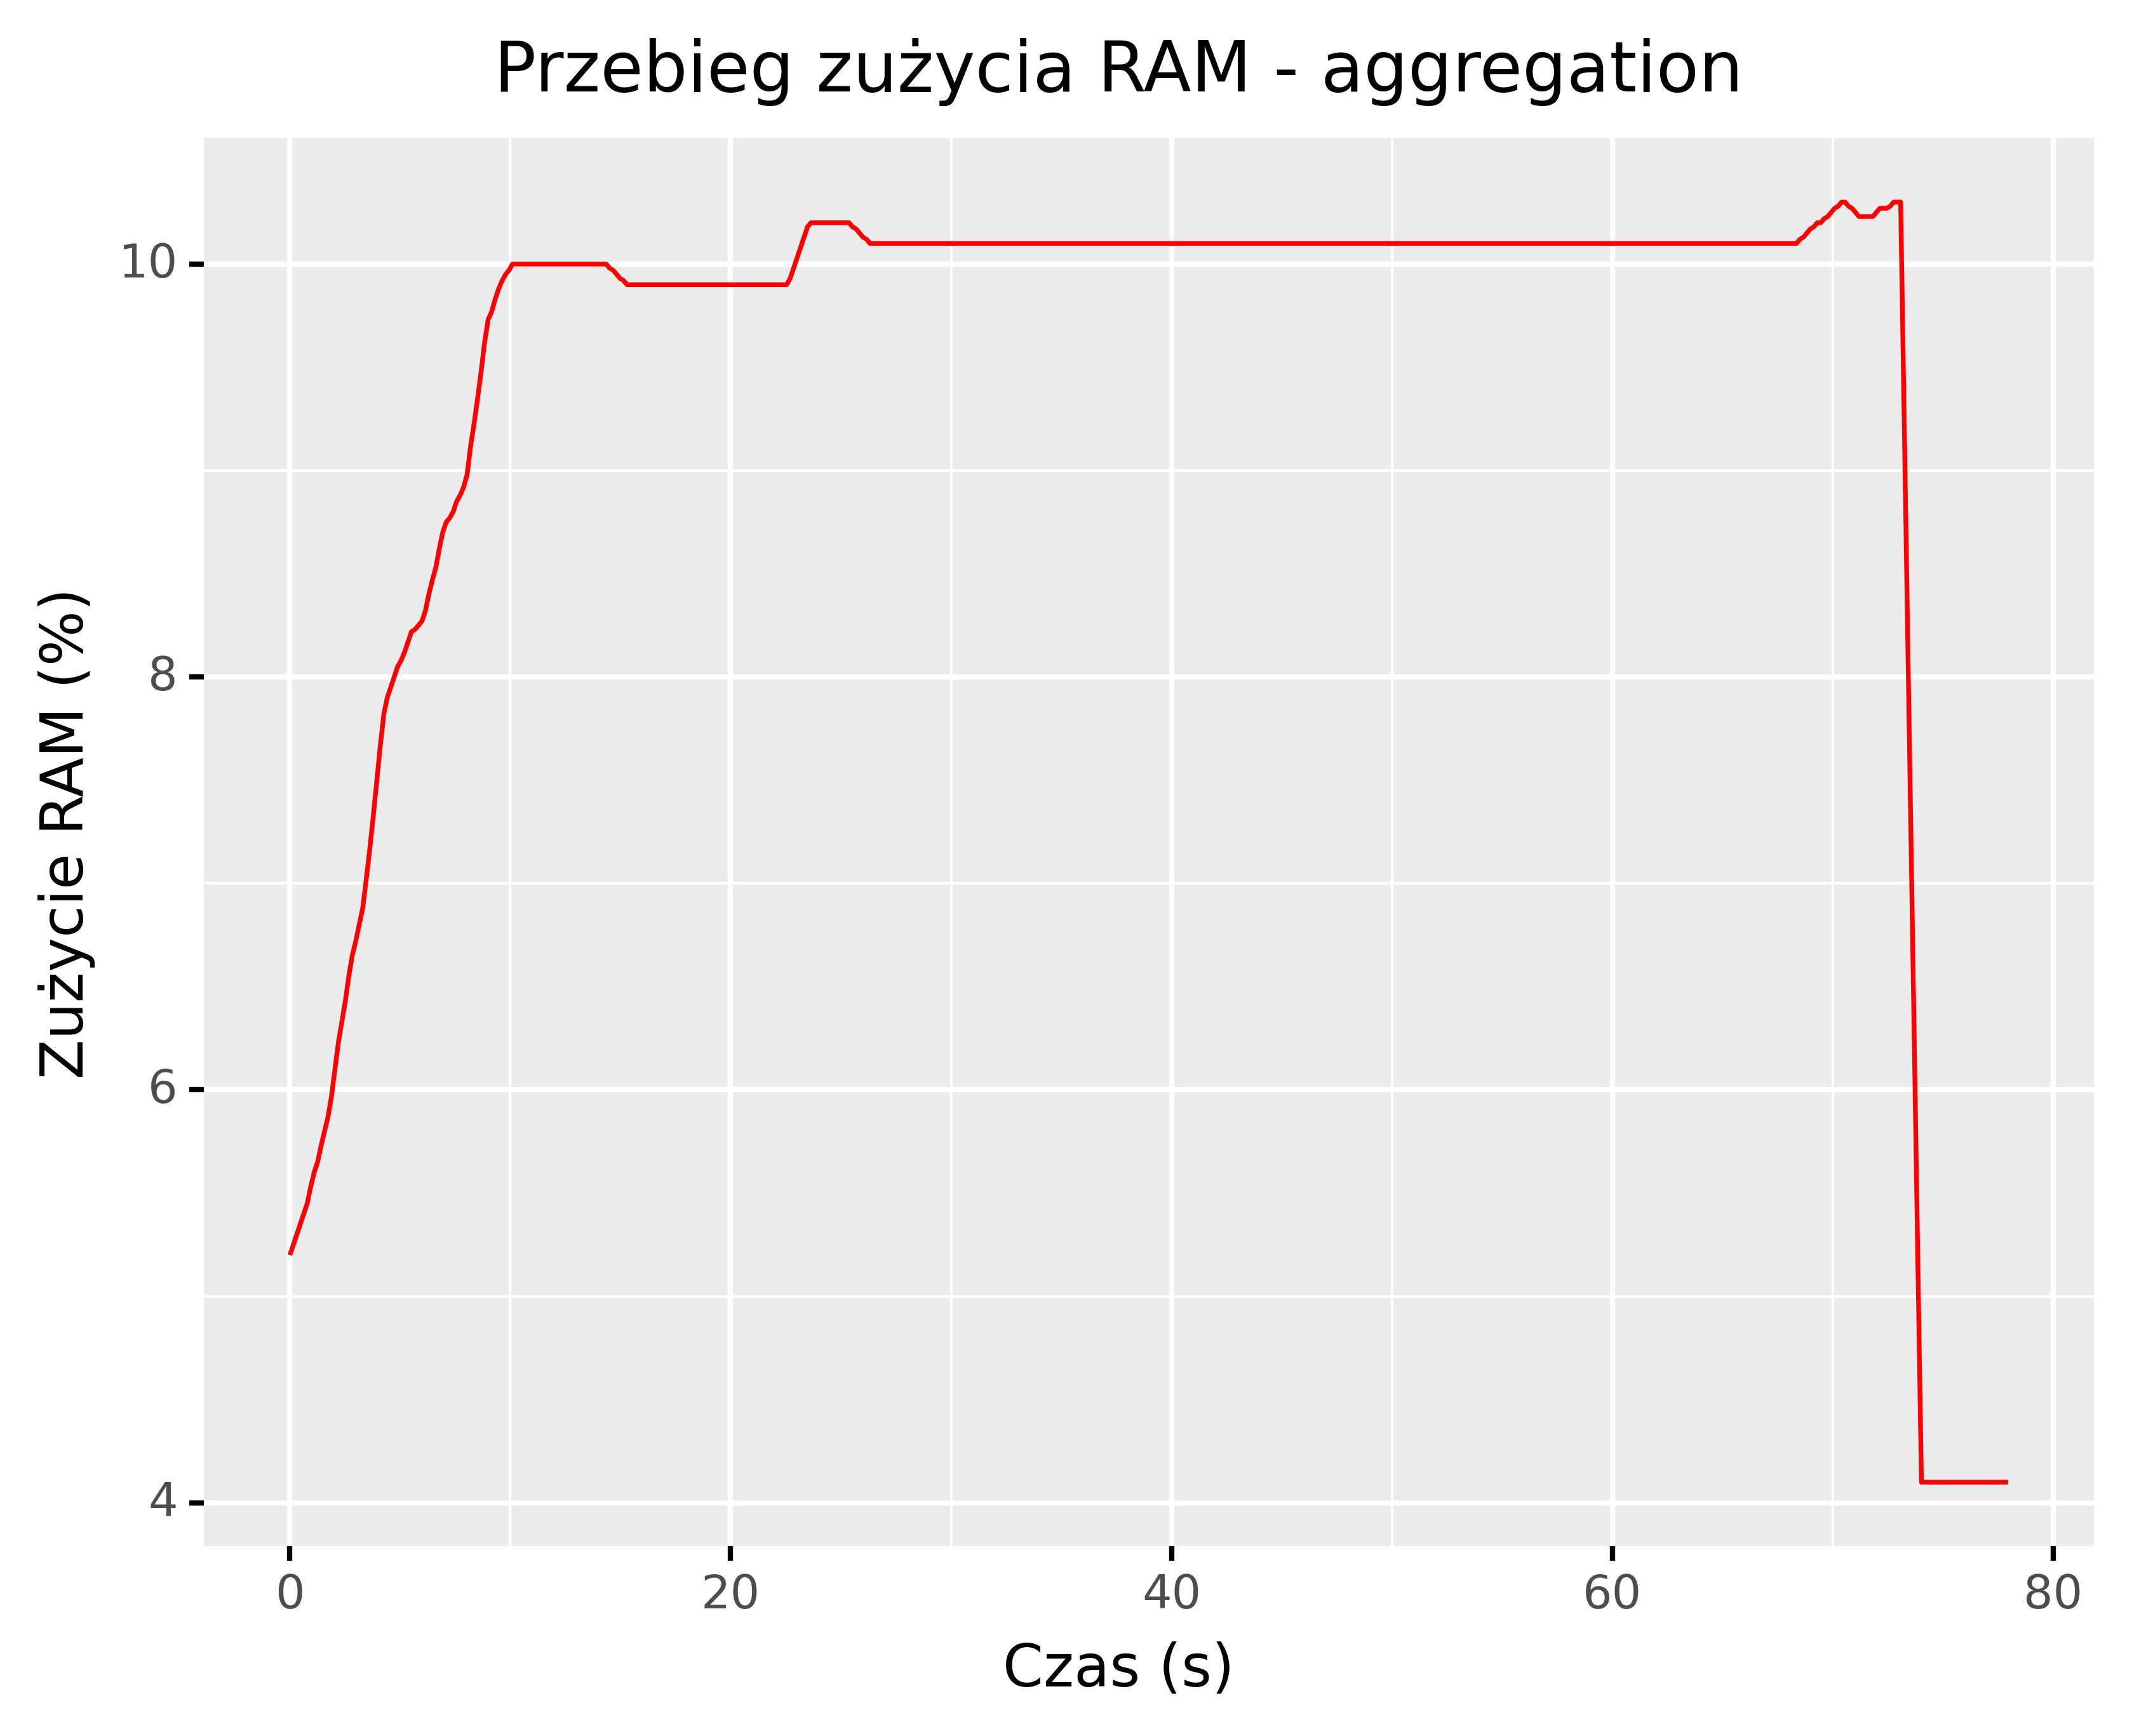
\includegraphics[width=0.5\textwidth]{figures/04-opis-danych/aggregation_smooth_6_ram_snapshot_1.png}\label{aggregation_smooth_6:f2}}
  \caption{Przykładowy wygładzony wykres zużycia zasobów dla agregacji (snapshot = 1, okno 1 sekundowe)}
  \label{aggregation_smooth_6}
\end{figure}

\begin{figure}[H]
  \centering
  \subfloat[CPU]{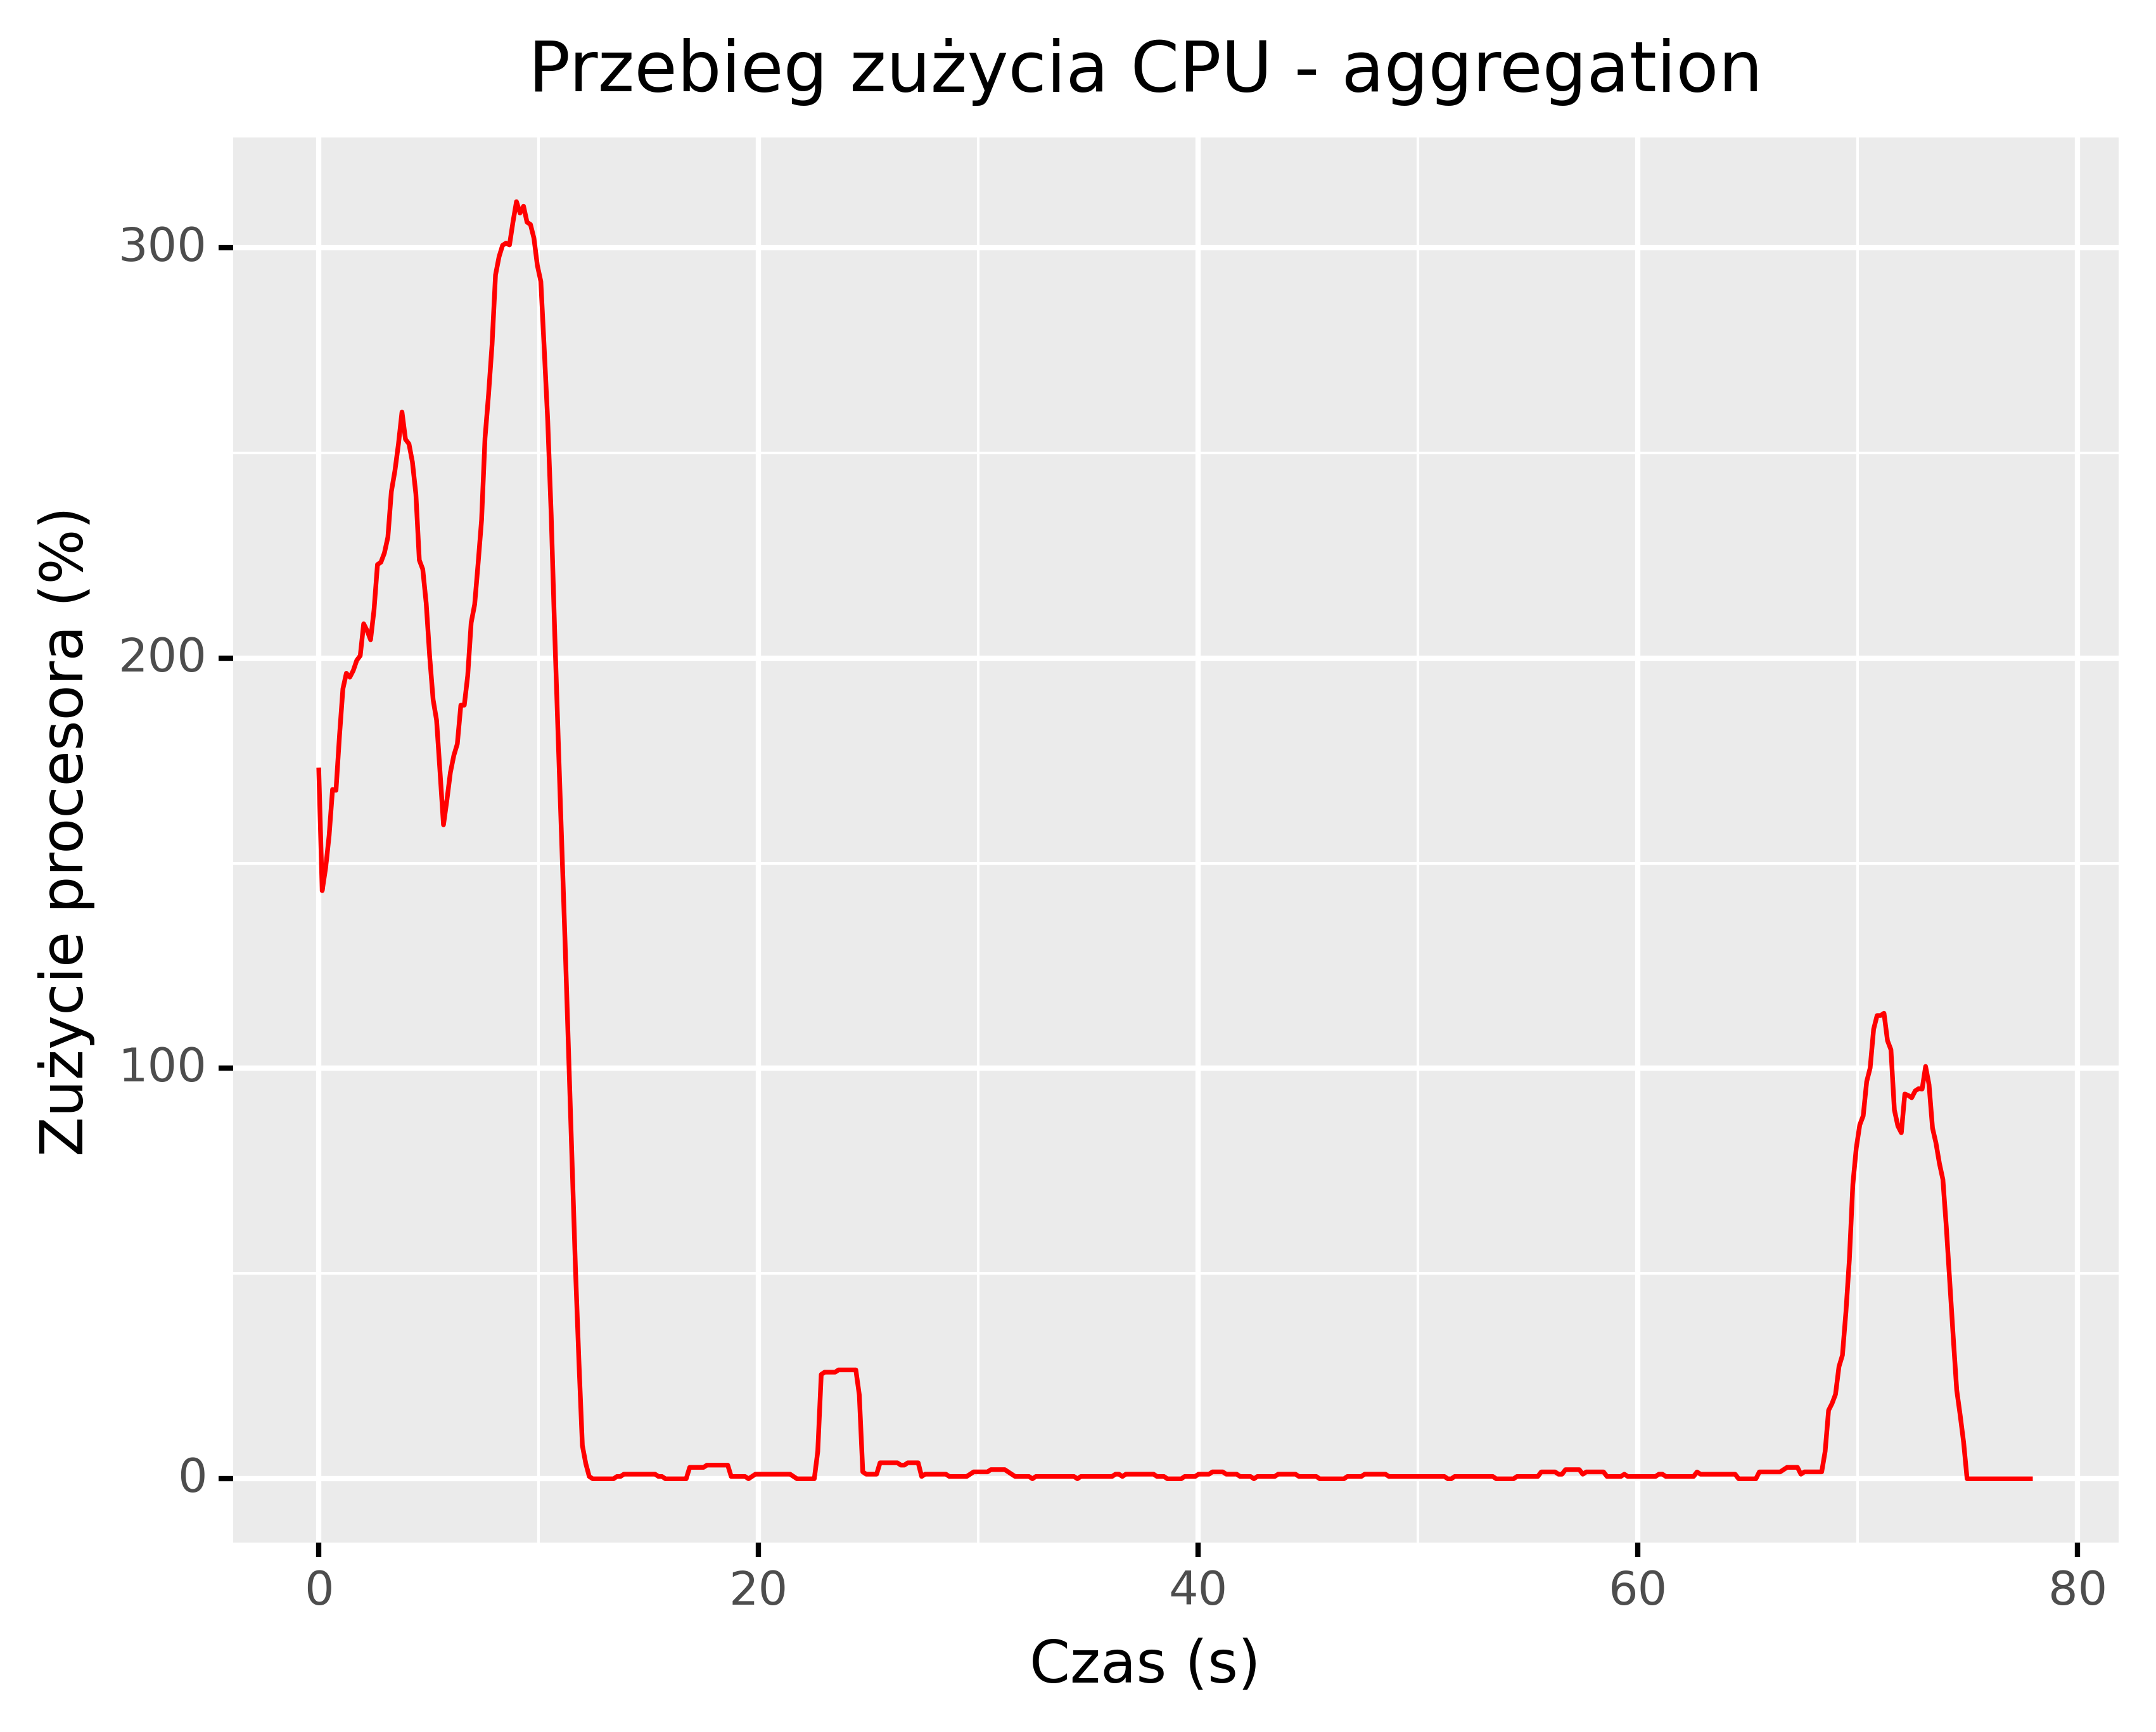
\includegraphics[width=0.5\textwidth]{figures/04-opis-danych/aggregation_smooth_12_cpu_snapshot_1.png}\label{aggregation_smooth_12:f1}}
  \hfill
  \subfloat[RAM]{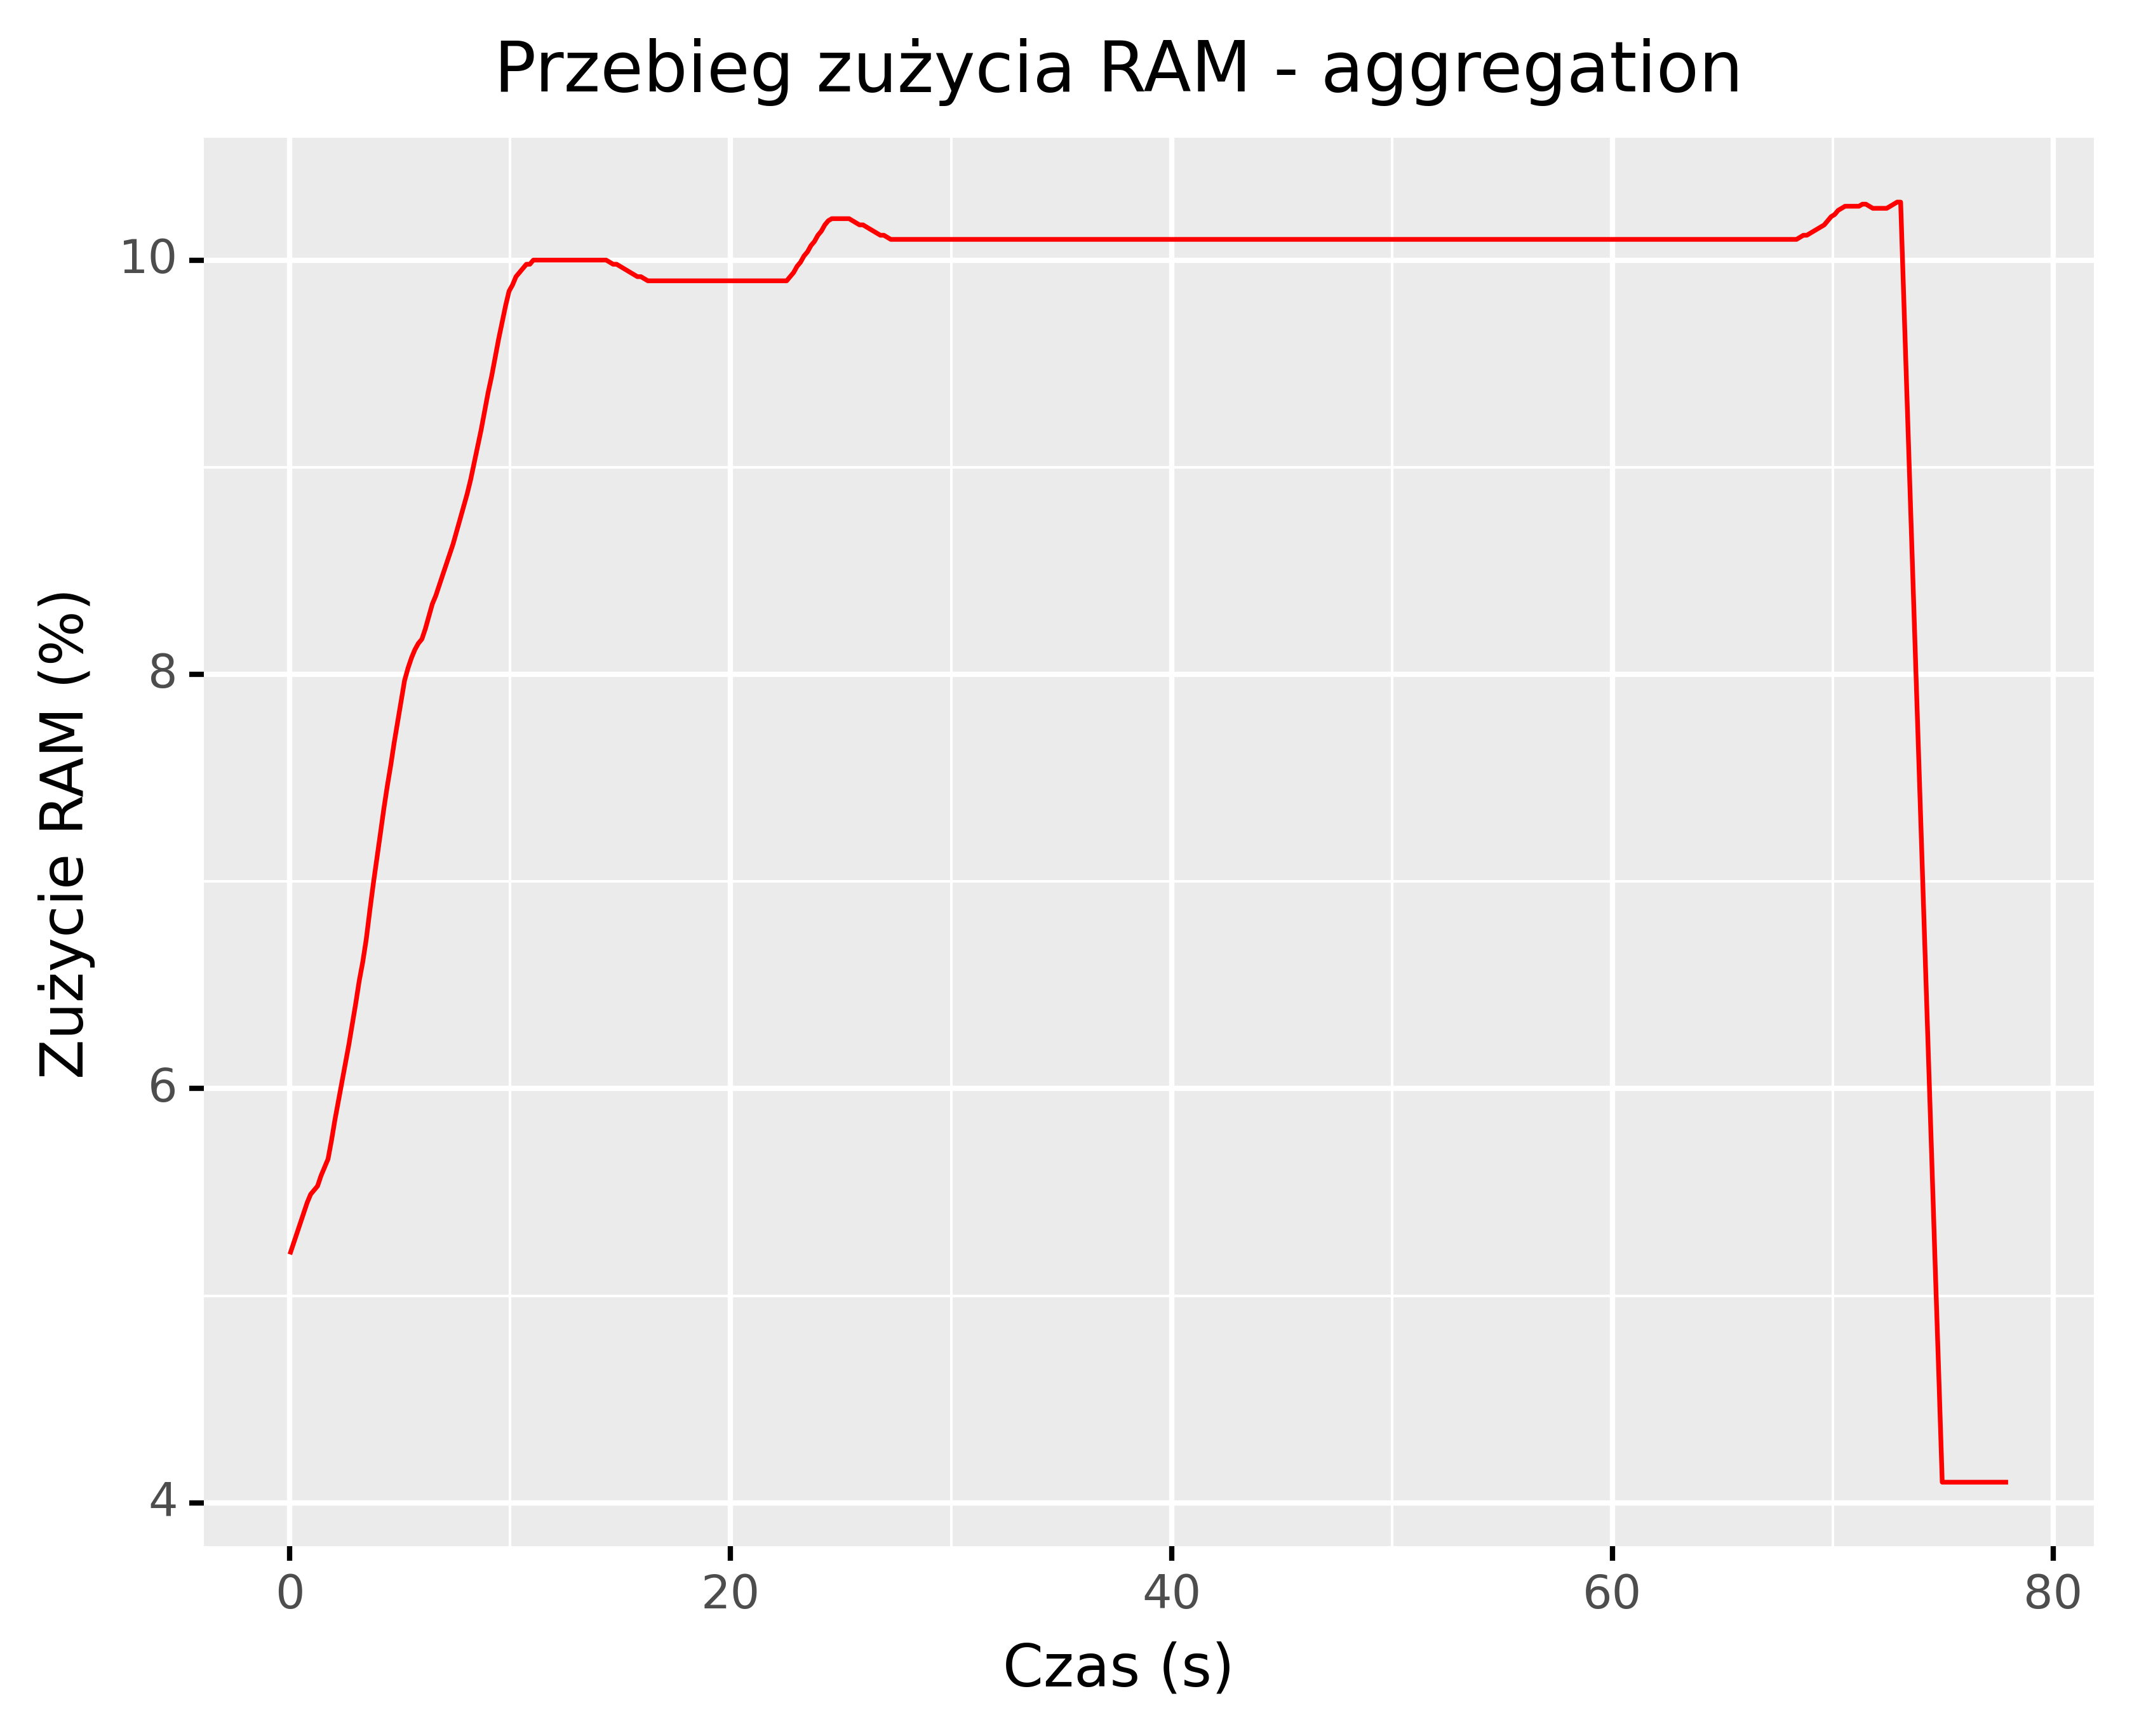
\includegraphics[width=0.5\textwidth]{figures/04-opis-danych/aggregation_smooth_12_ram_snapshot_1.png}\label{aggregation_smooth_12:f2}}
  \caption{Przykładowy wygładzony wykres zużycia zasobów dla agregacji (snapshot = 1, okno 2 sekundowe)}
  \label{aggregation_smooth_12}
\end{figure}

\begin{figure}[H]
  \centering
  \subfloat[CPU]{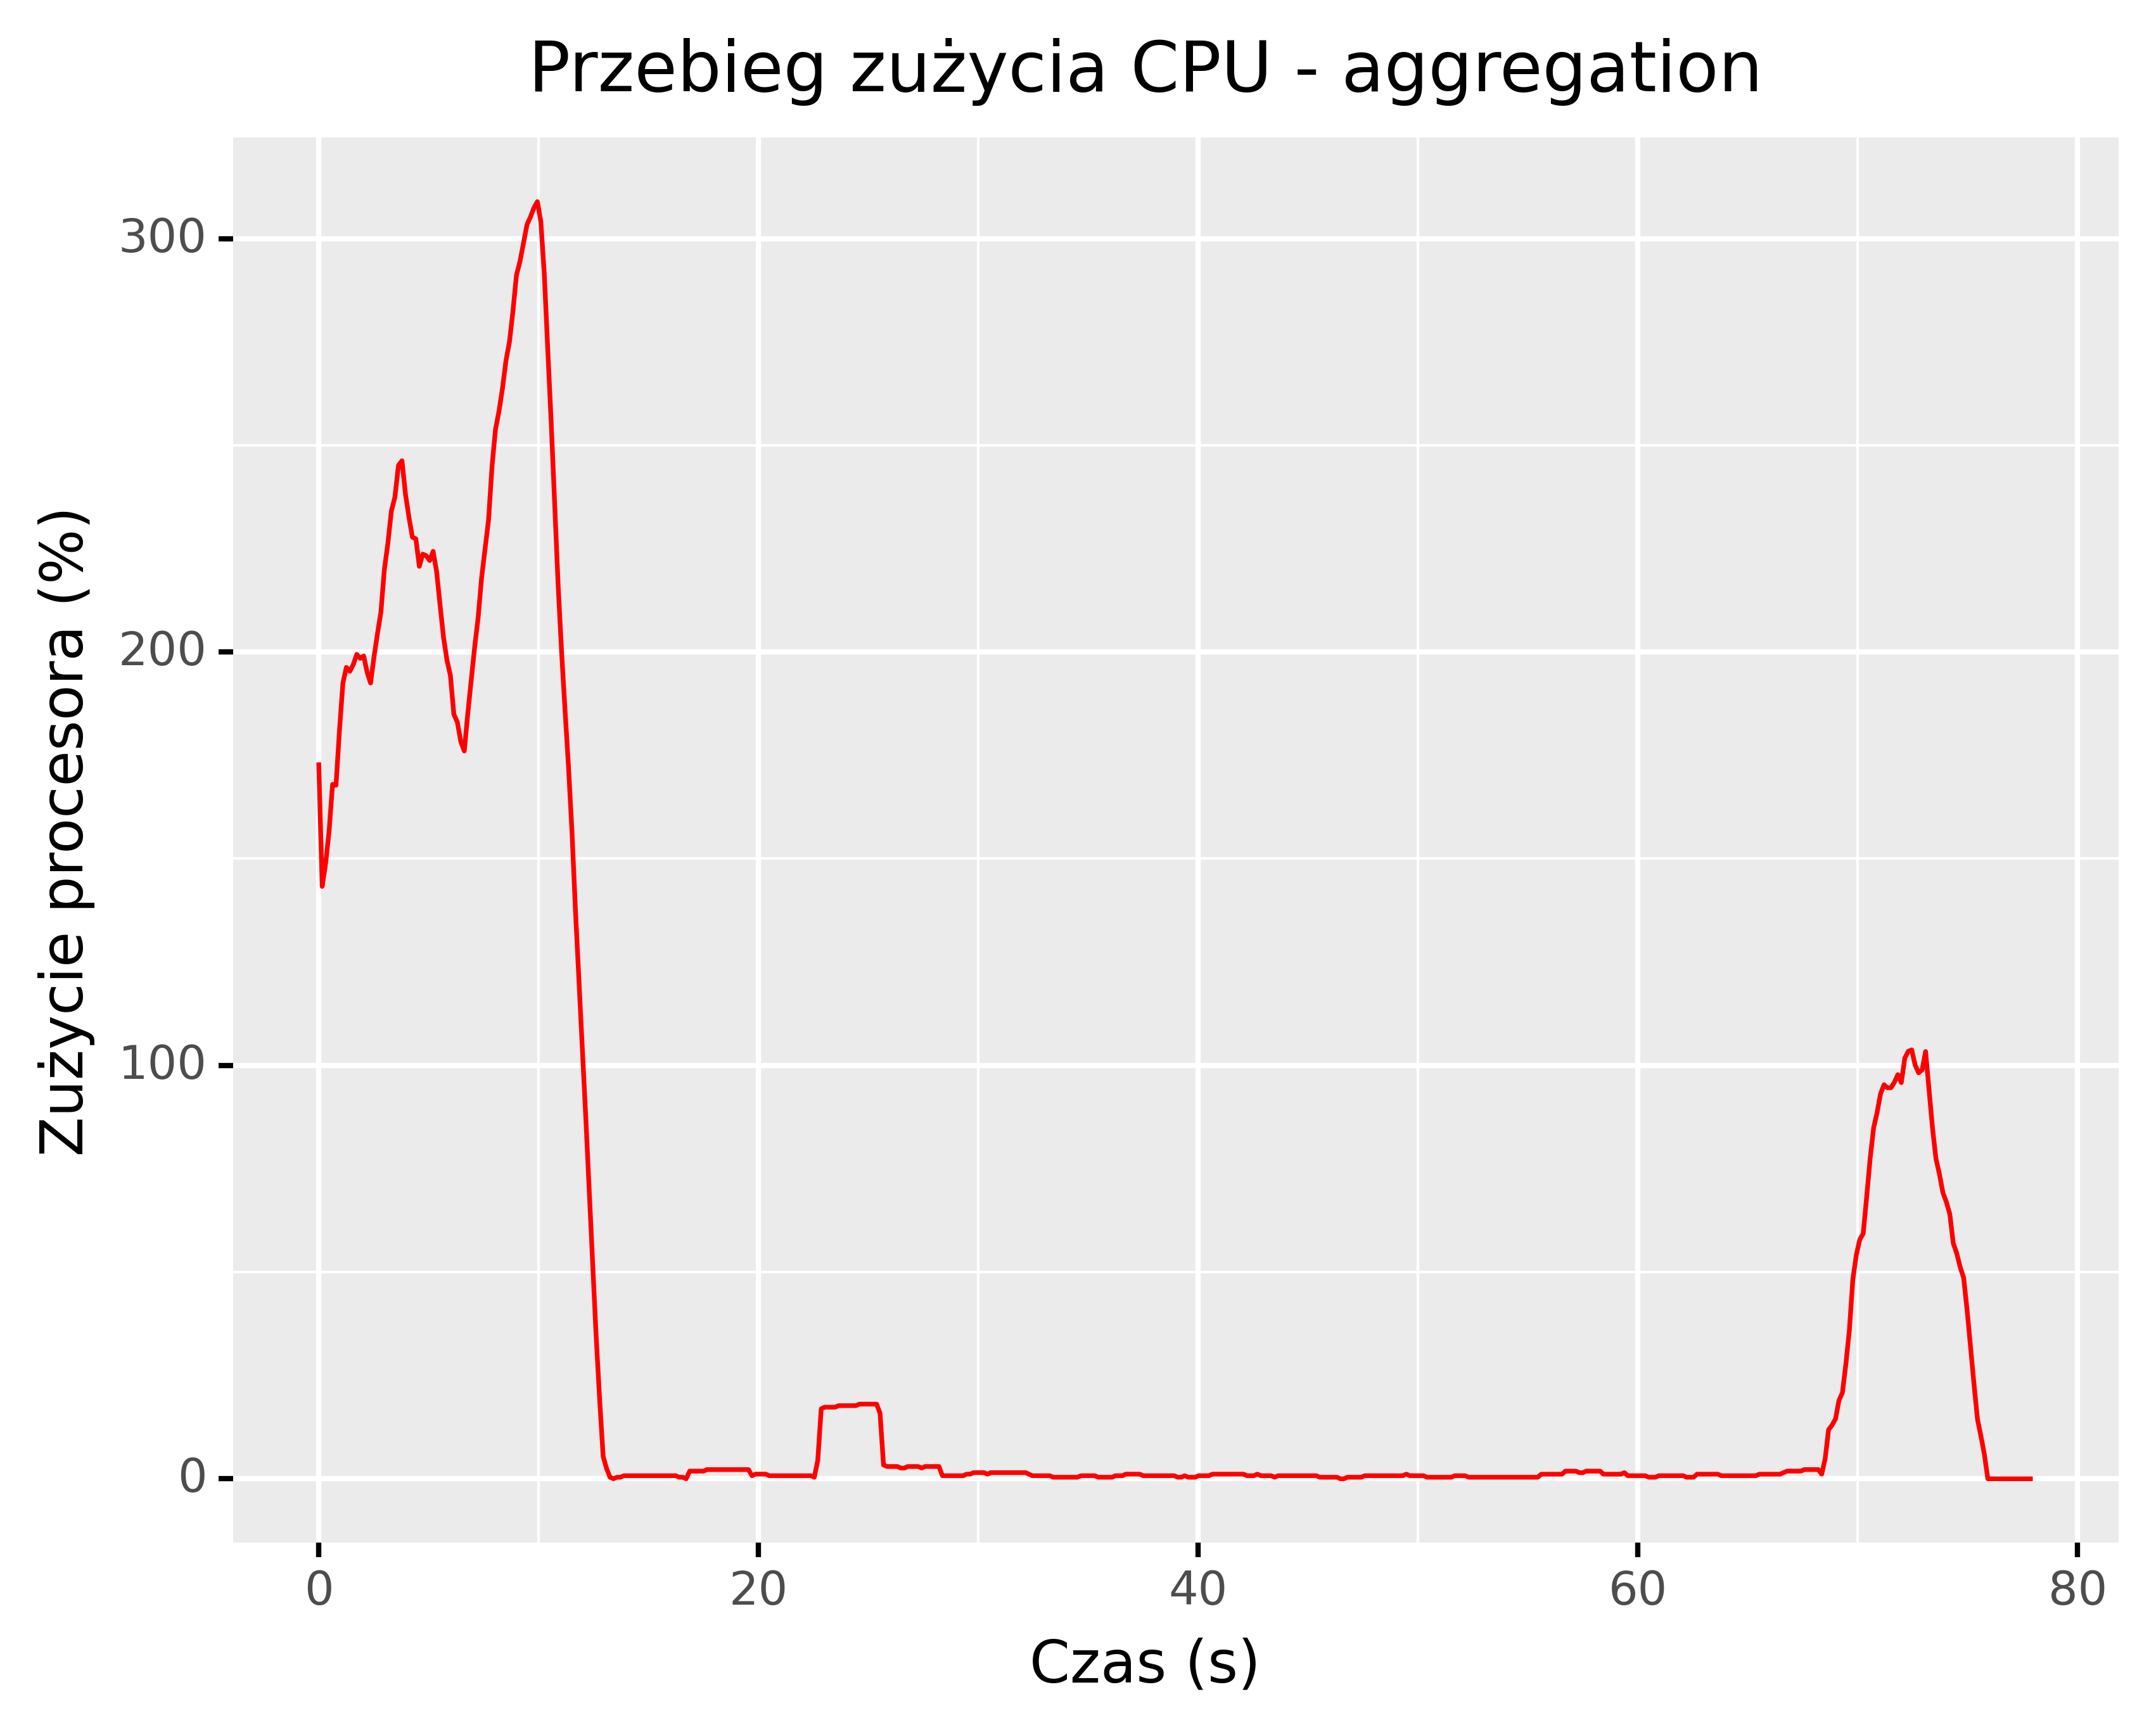
\includegraphics[width=0.5\textwidth]{figures/04-opis-danych/aggregation_smooth_18_cpu_snapshot_1.png}\label{aggregation_smooth_18:f1}}
  \hfill
  \subfloat[RAM]{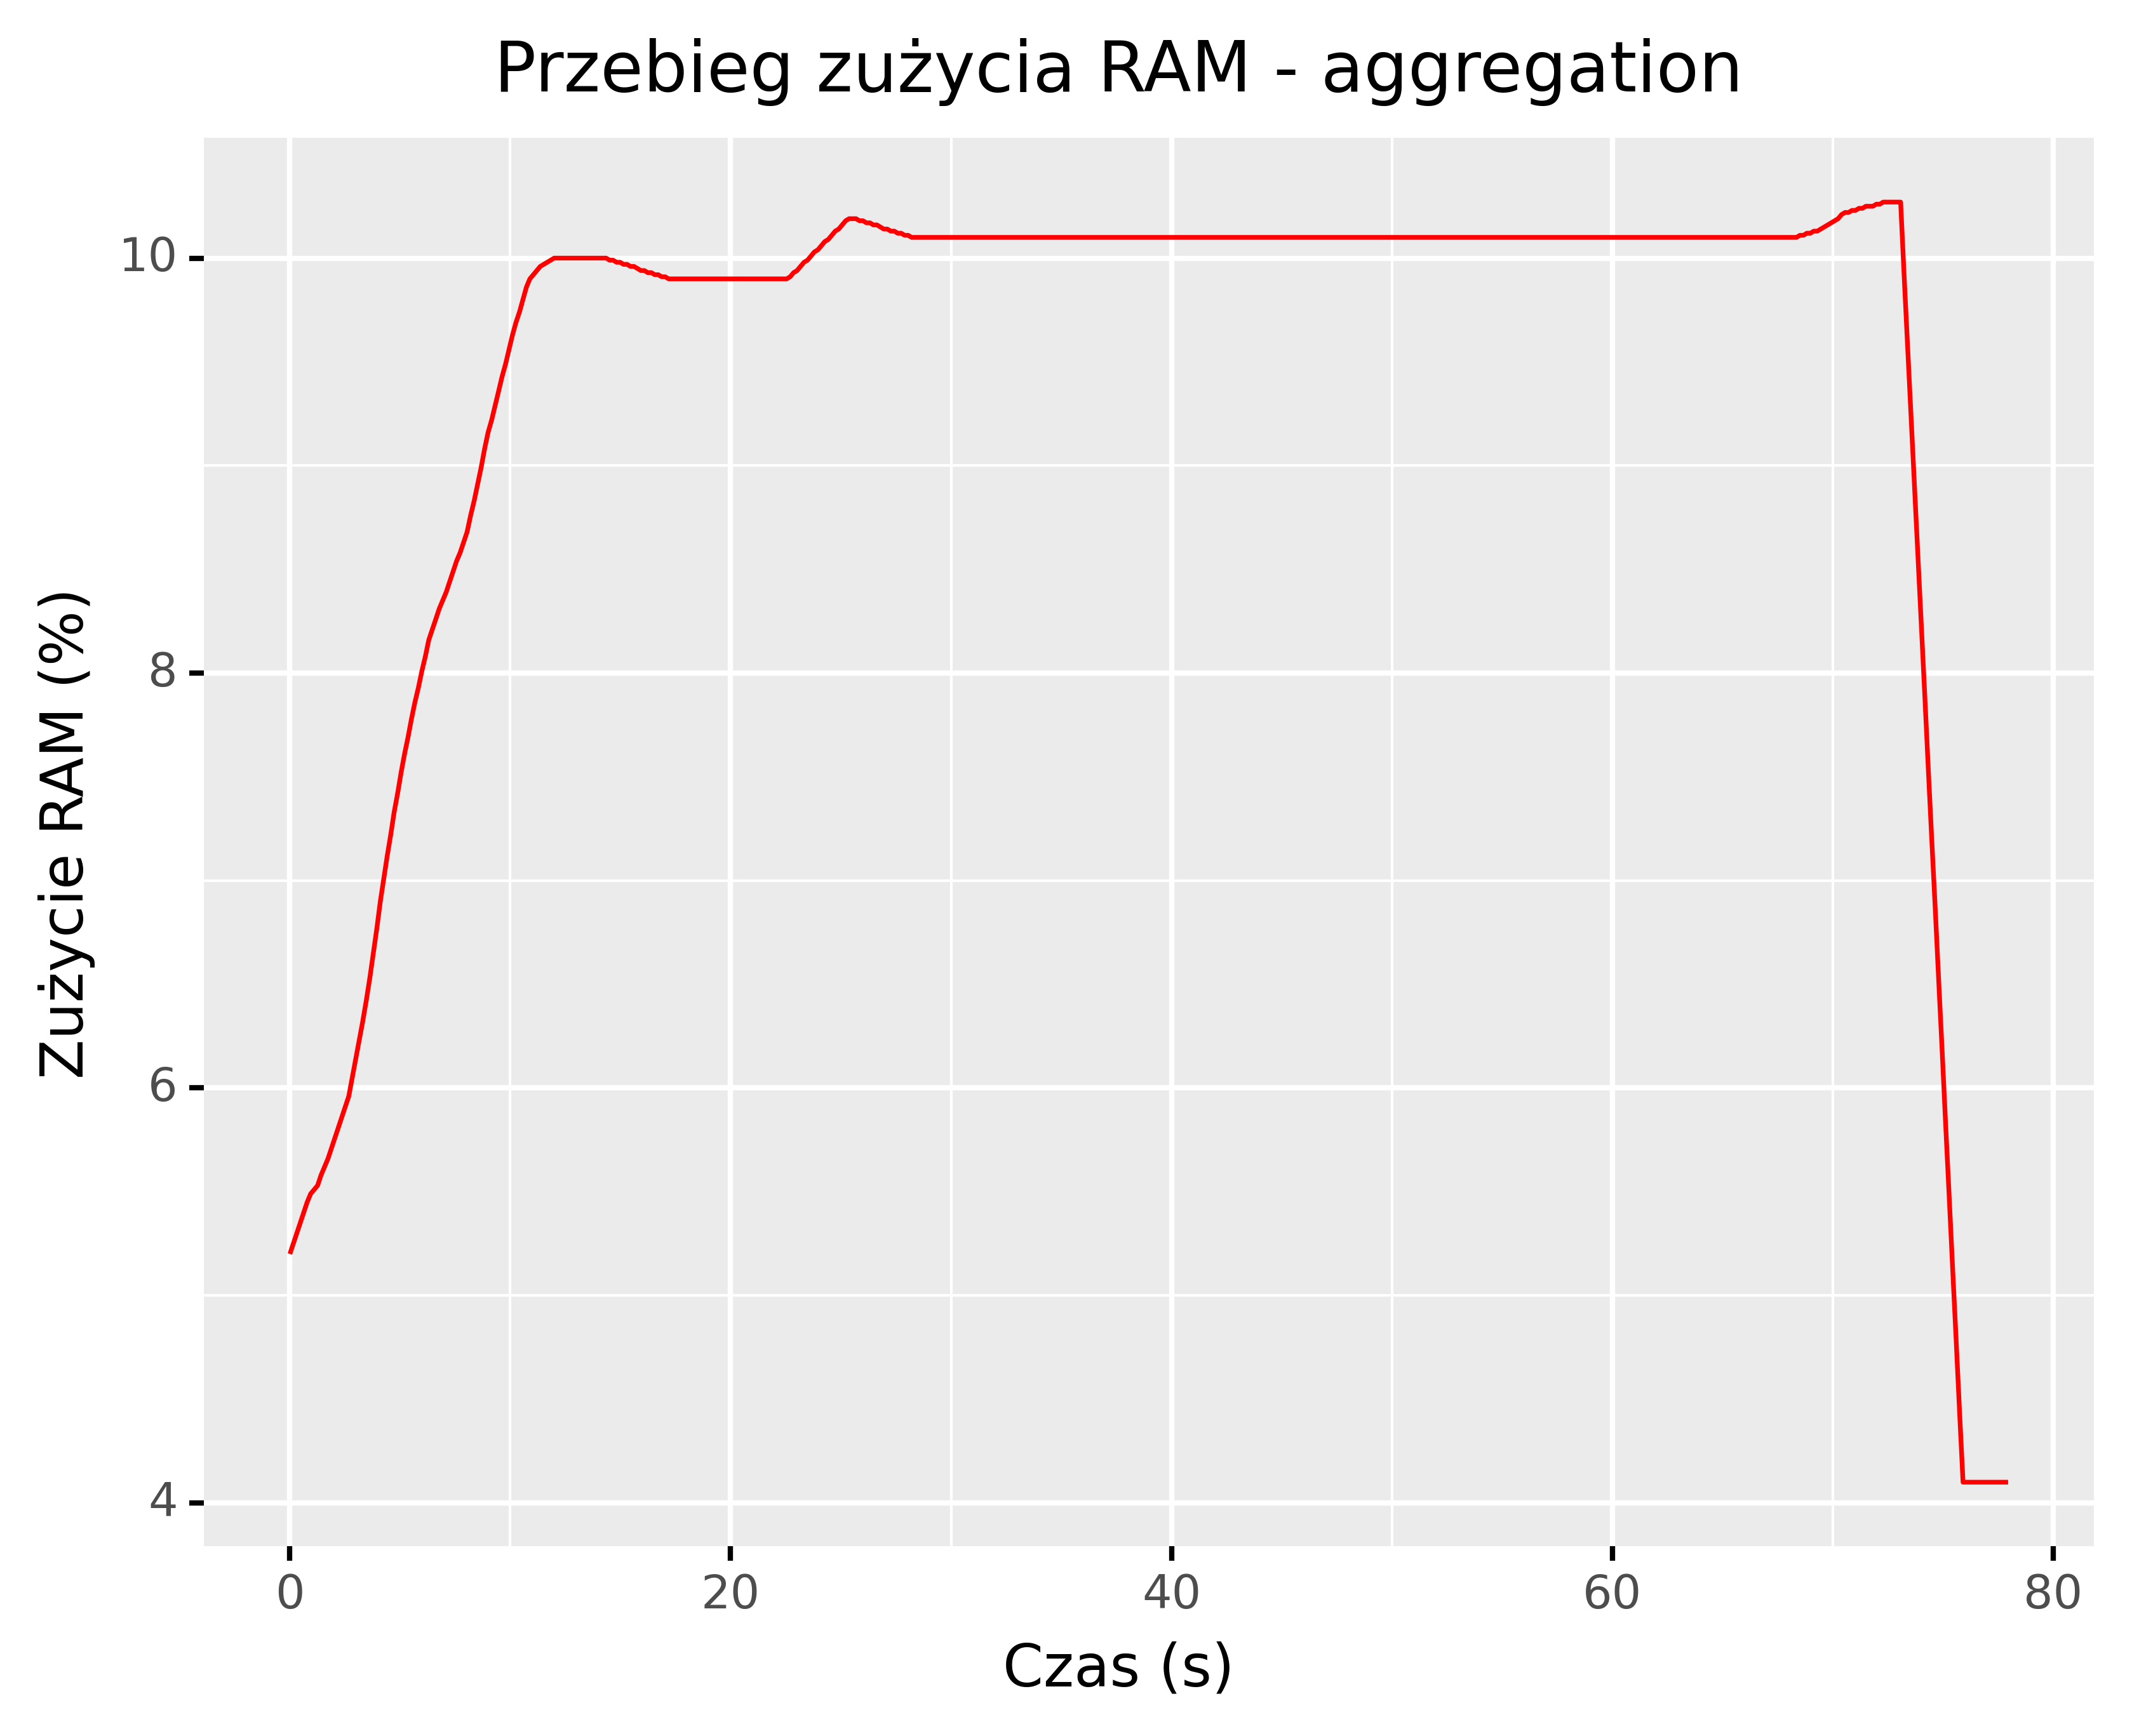
\includegraphics[width=0.5\textwidth]{figures/04-opis-danych/aggregation_smooth_18_ram_snapshot_1.png}\label{aggregation_smooth_18:f2}}
  \caption{Przykładowy wygładzony wykres zużycia zasobów dla agregacji (snapshot = 1, okno 3 sekundowe)}
  \label{aggregation_smooth_18}
\end{figure}

Po wykonaniu transformacji można zauważyć, że wykresy są bardziej stabilne (mniej dużej ilości skoków wartości w małym przedziale czasowym). Rysunki od \ref{aggregation_smooth_6} do \ref{aggregation_smooth_18} pokazują na przykładzie agregacji wyniki dla kolejno 6, 12 i 18 próbek (czyli 1, 2, 3 sekundy). Ostatecznie nie chcąc przesadzić będziemy korzystali prawdopodobnie z oknem 1 sekundowym, żeby nie stracić zbyt wielu informacji, co mogłoby się zdarzyć używając zbyt dużego okna. Przykładowo na rysunku CPU \ref{aggregation_smooth_18} widać w porównaniu z rysunkiem \ref{aggregation_smooth_6} mocno zmniejszony szczyt w okolicy 25 sekundy.

Ostatnią transformacją przeprowadzoną na danych wejściowych jest normalizacja. Wykonana jest ona w celu sprawdzenia czy wybrane algorytmy liczenia podobieństwa między szeregami lepiej poradzą sobie z danymi niezmienionymi, czy jednak znormalizowanymi. W rozdziale \ref{section:norm} są po krotce opisane sposoby normalizacji i patrząc na nasze dane, możemy stwierdzić że nie mają one rozkładu normalnego. Widać to na wykresach \ref{aggregation_hist}, więc bazując na tym, że dla danych tego typu lepiej działa technika \textbf{Min-Max} zostanie ona wykorzystana na naszym zbiorze.

\begin{figure}[H]
  \centering
  \subfloat[CPU]{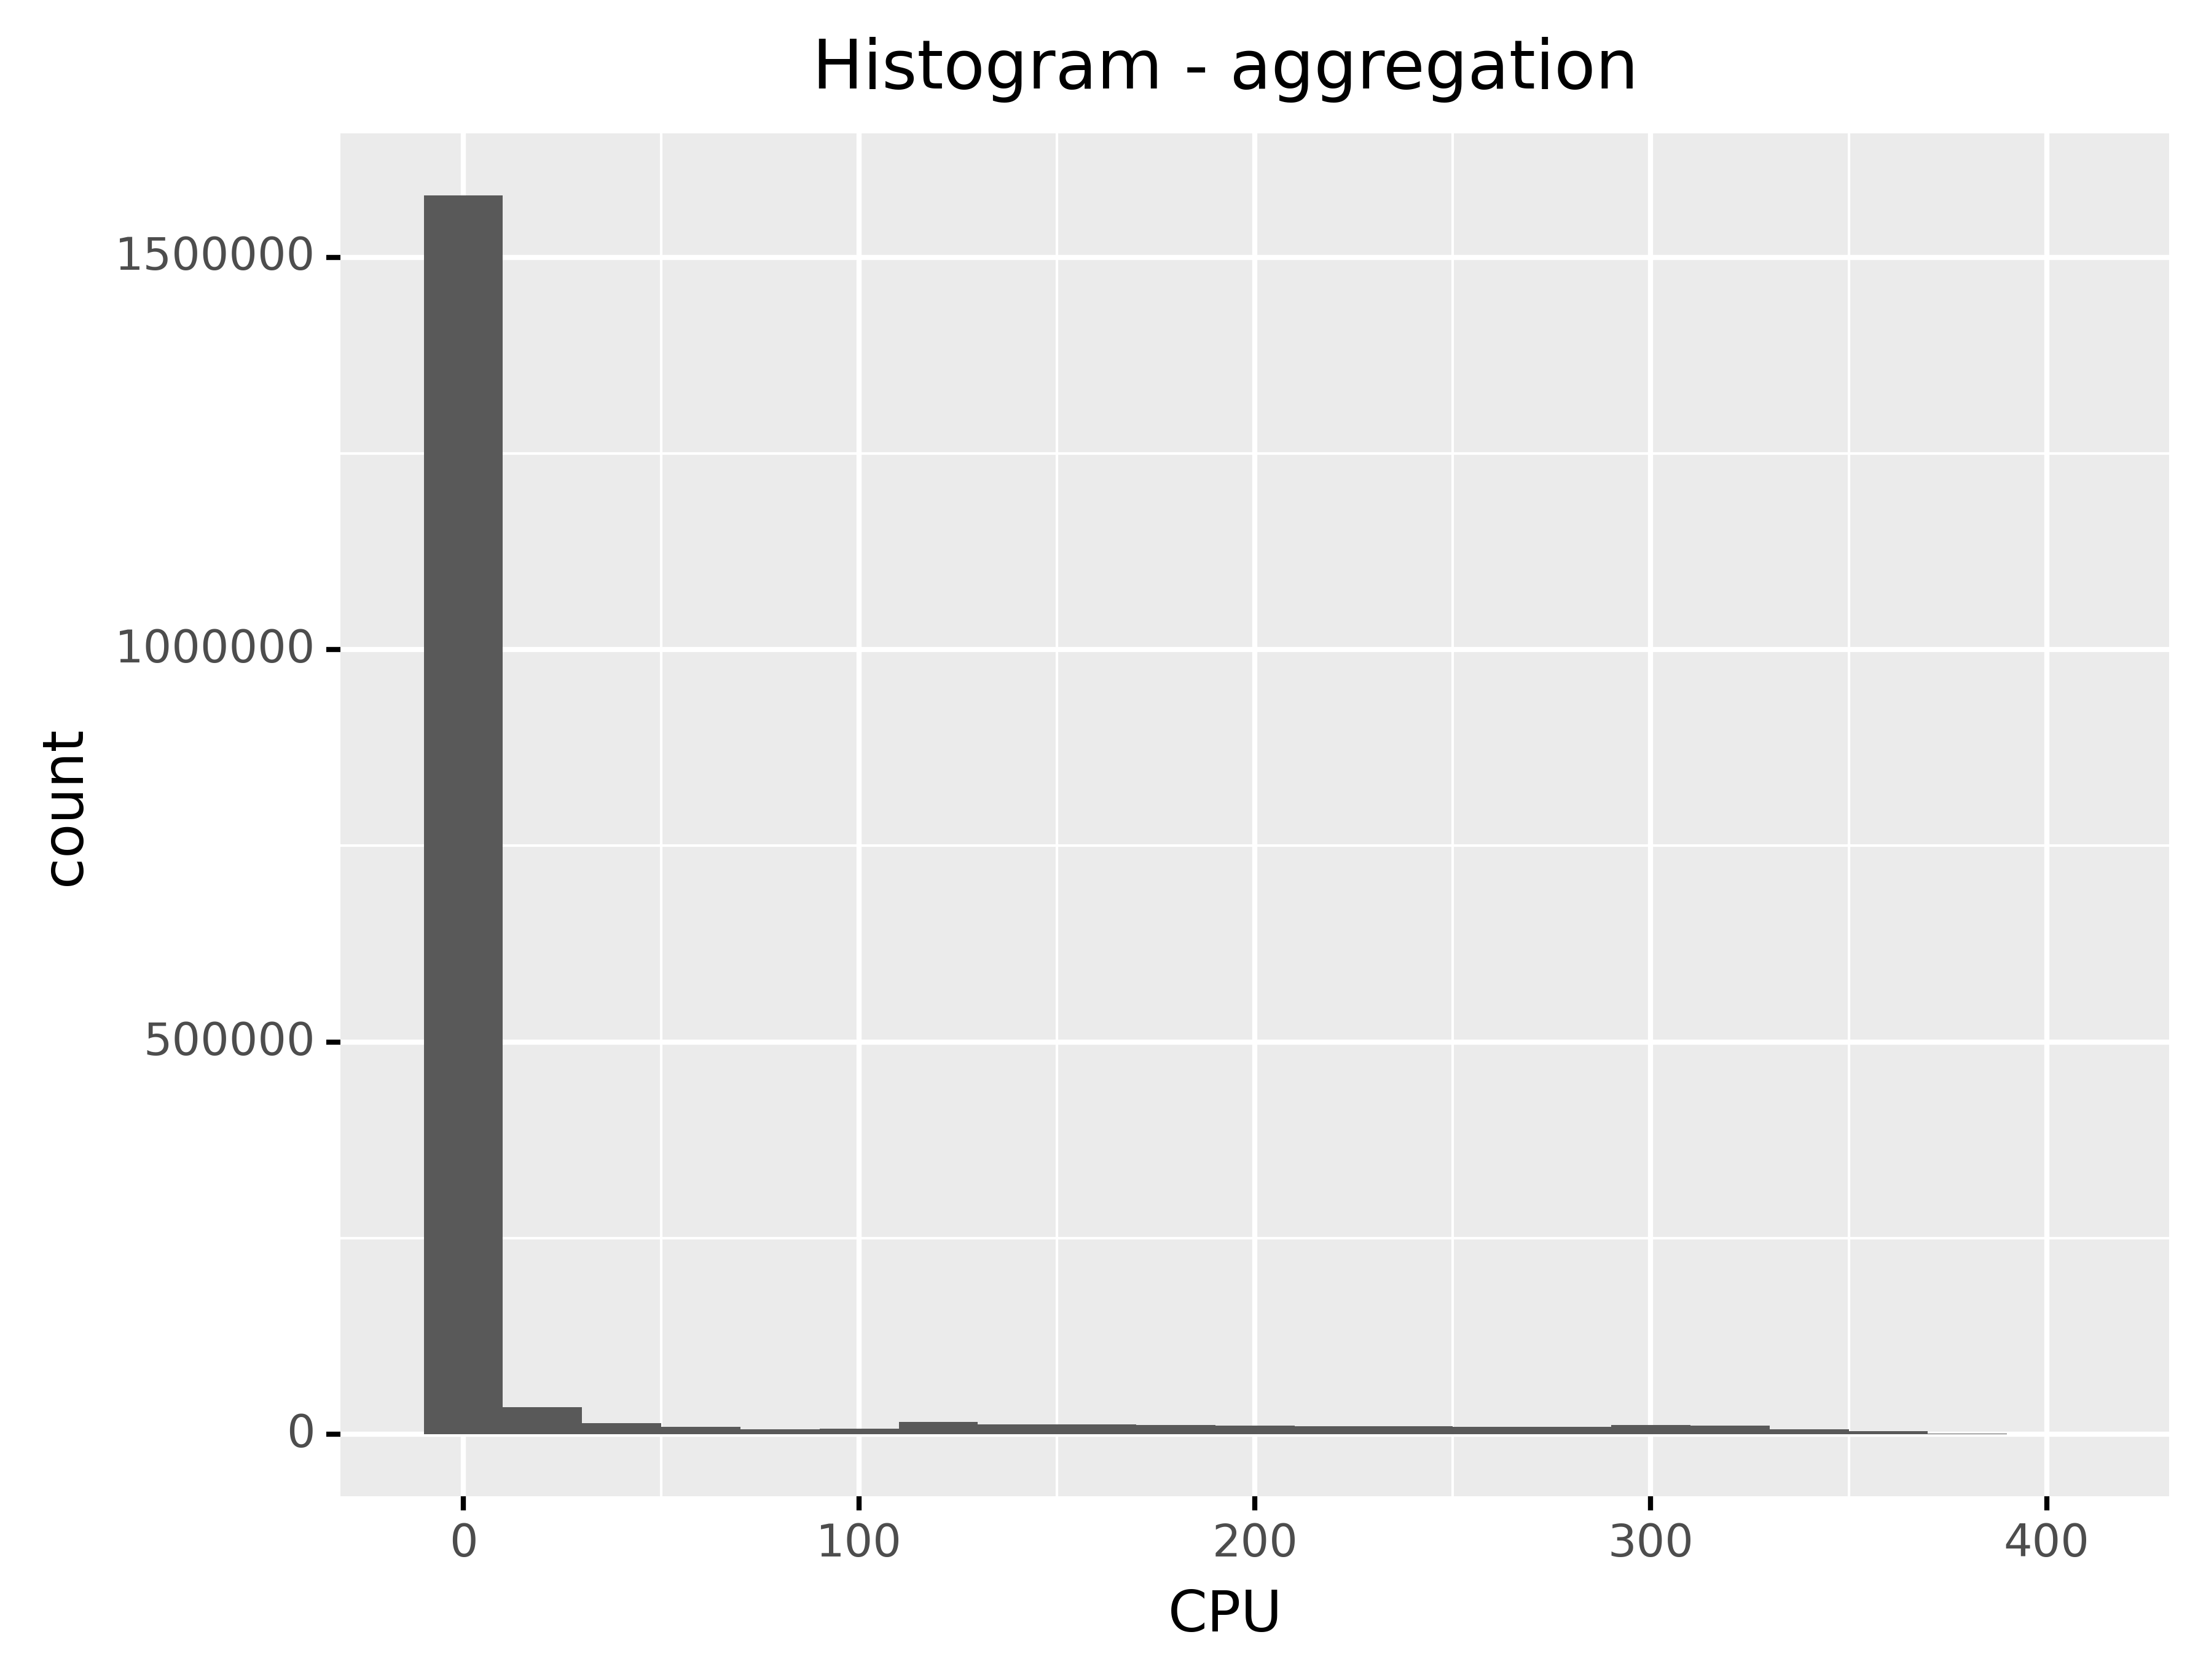
\includegraphics[width=0.5\textwidth]{figures/04-opis-danych/aggregation_hist_cpu.png}\label{aggregation_hist:cpu}}
  \hfill
  \subfloat[RAM]{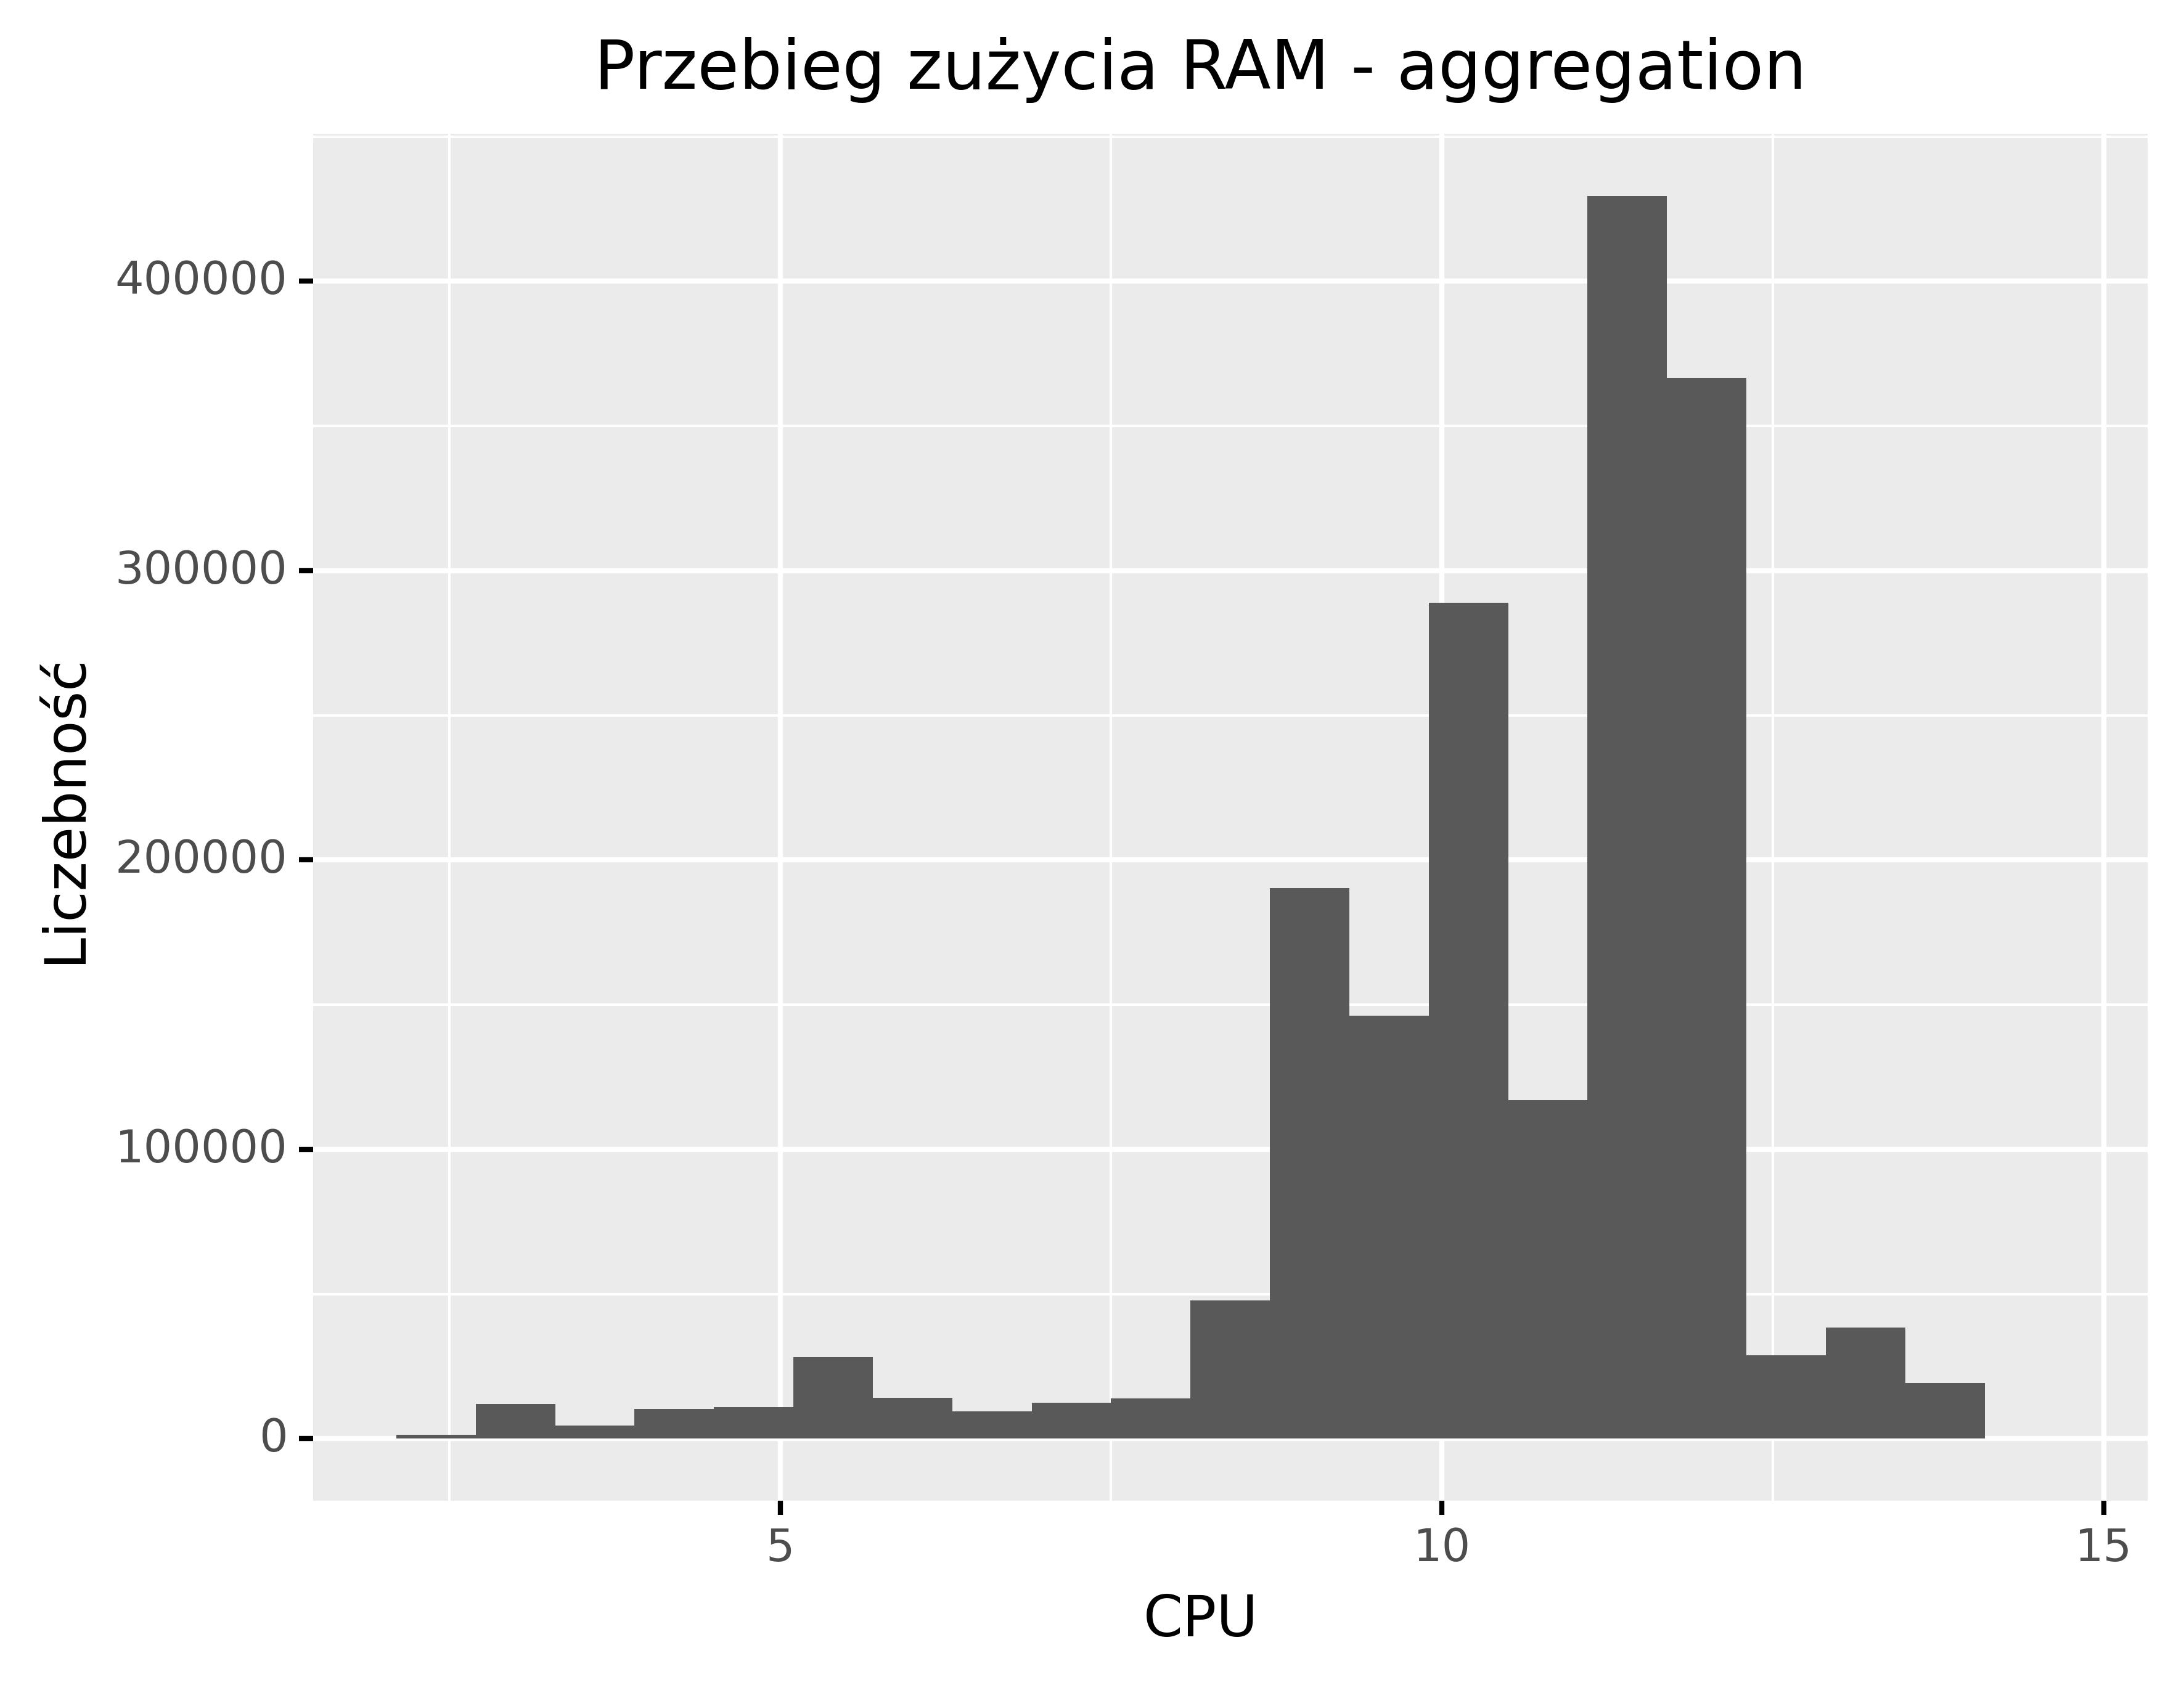
\includegraphics[width=0.5\textwidth]{figures/04-opis-danych/aggregation_hist_ram.png}\label{aggregation_hist:ram}}
  \caption{rozkład danych dla agregacji}
  \label{aggregation_hist}
\end{figure}


\begin{figure}[H]
  \centering
  \subfloat[CPU]{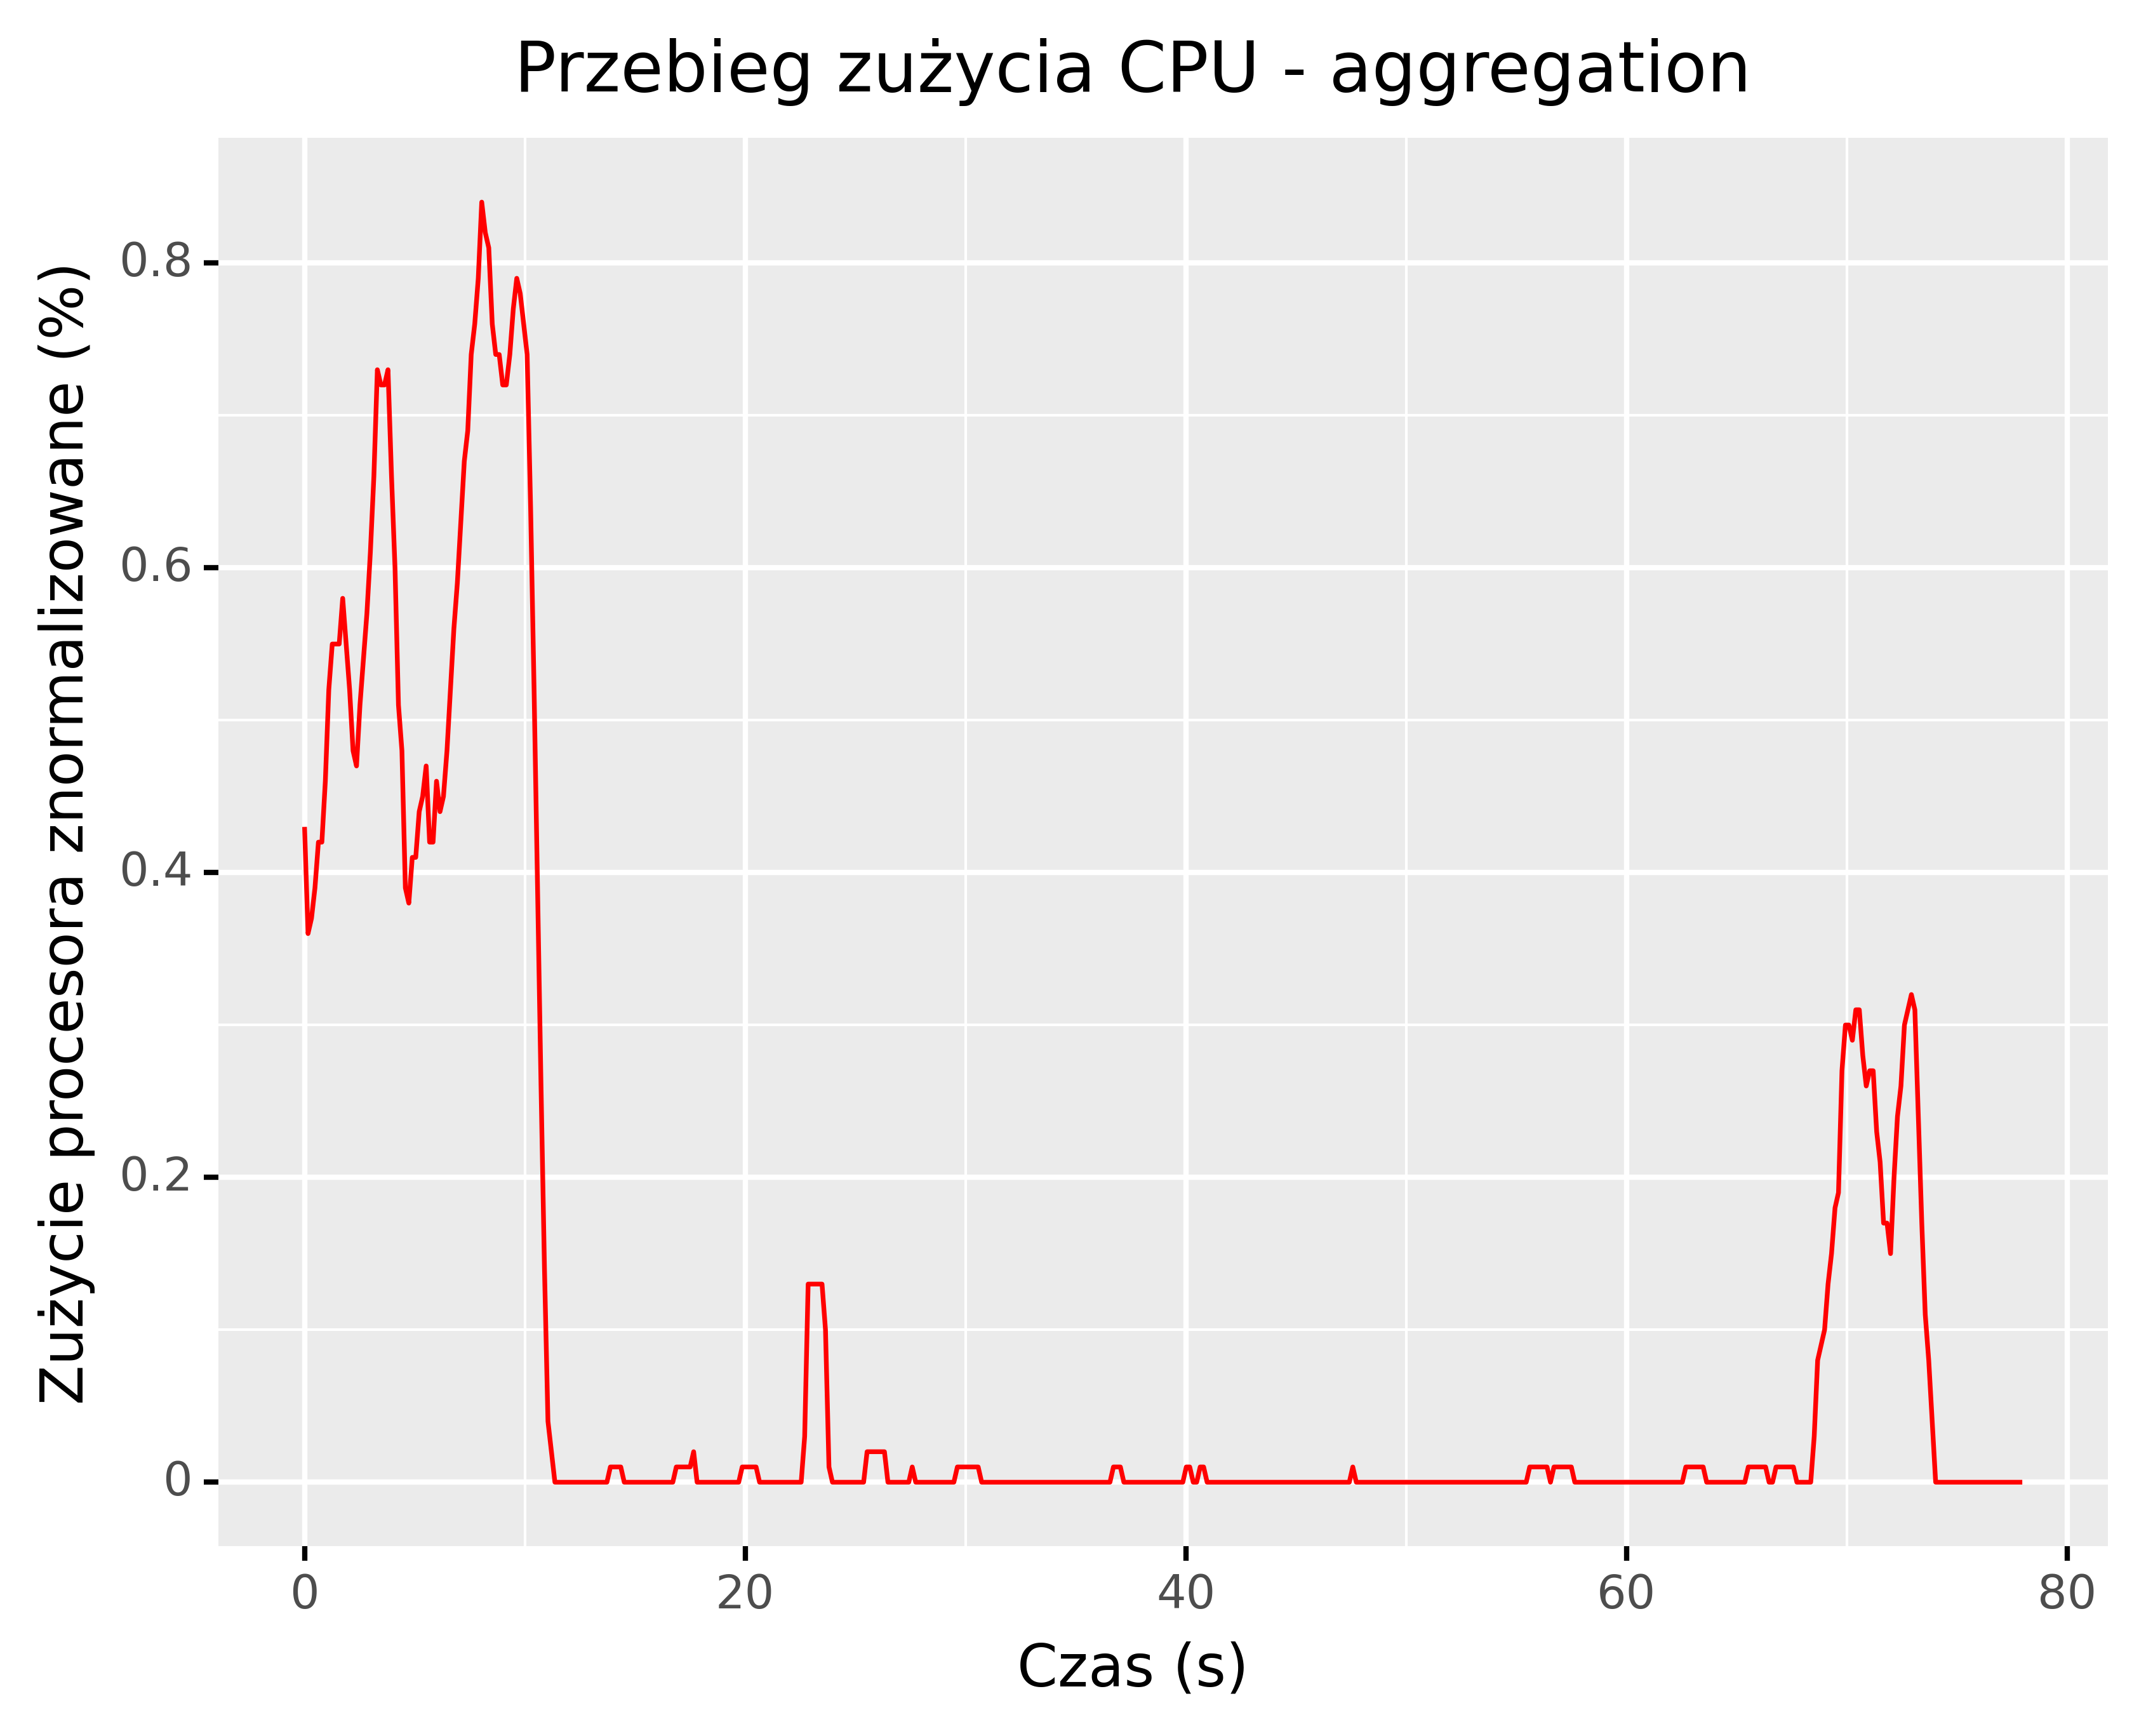
\includegraphics[width=0.5\textwidth]{figures/04-opis-danych/aggregation_smooth_normalized_cpu_snapshot_1.png}\label{aggregation_normalized:cpu}}
  \hfill
  \subfloat[RAM]{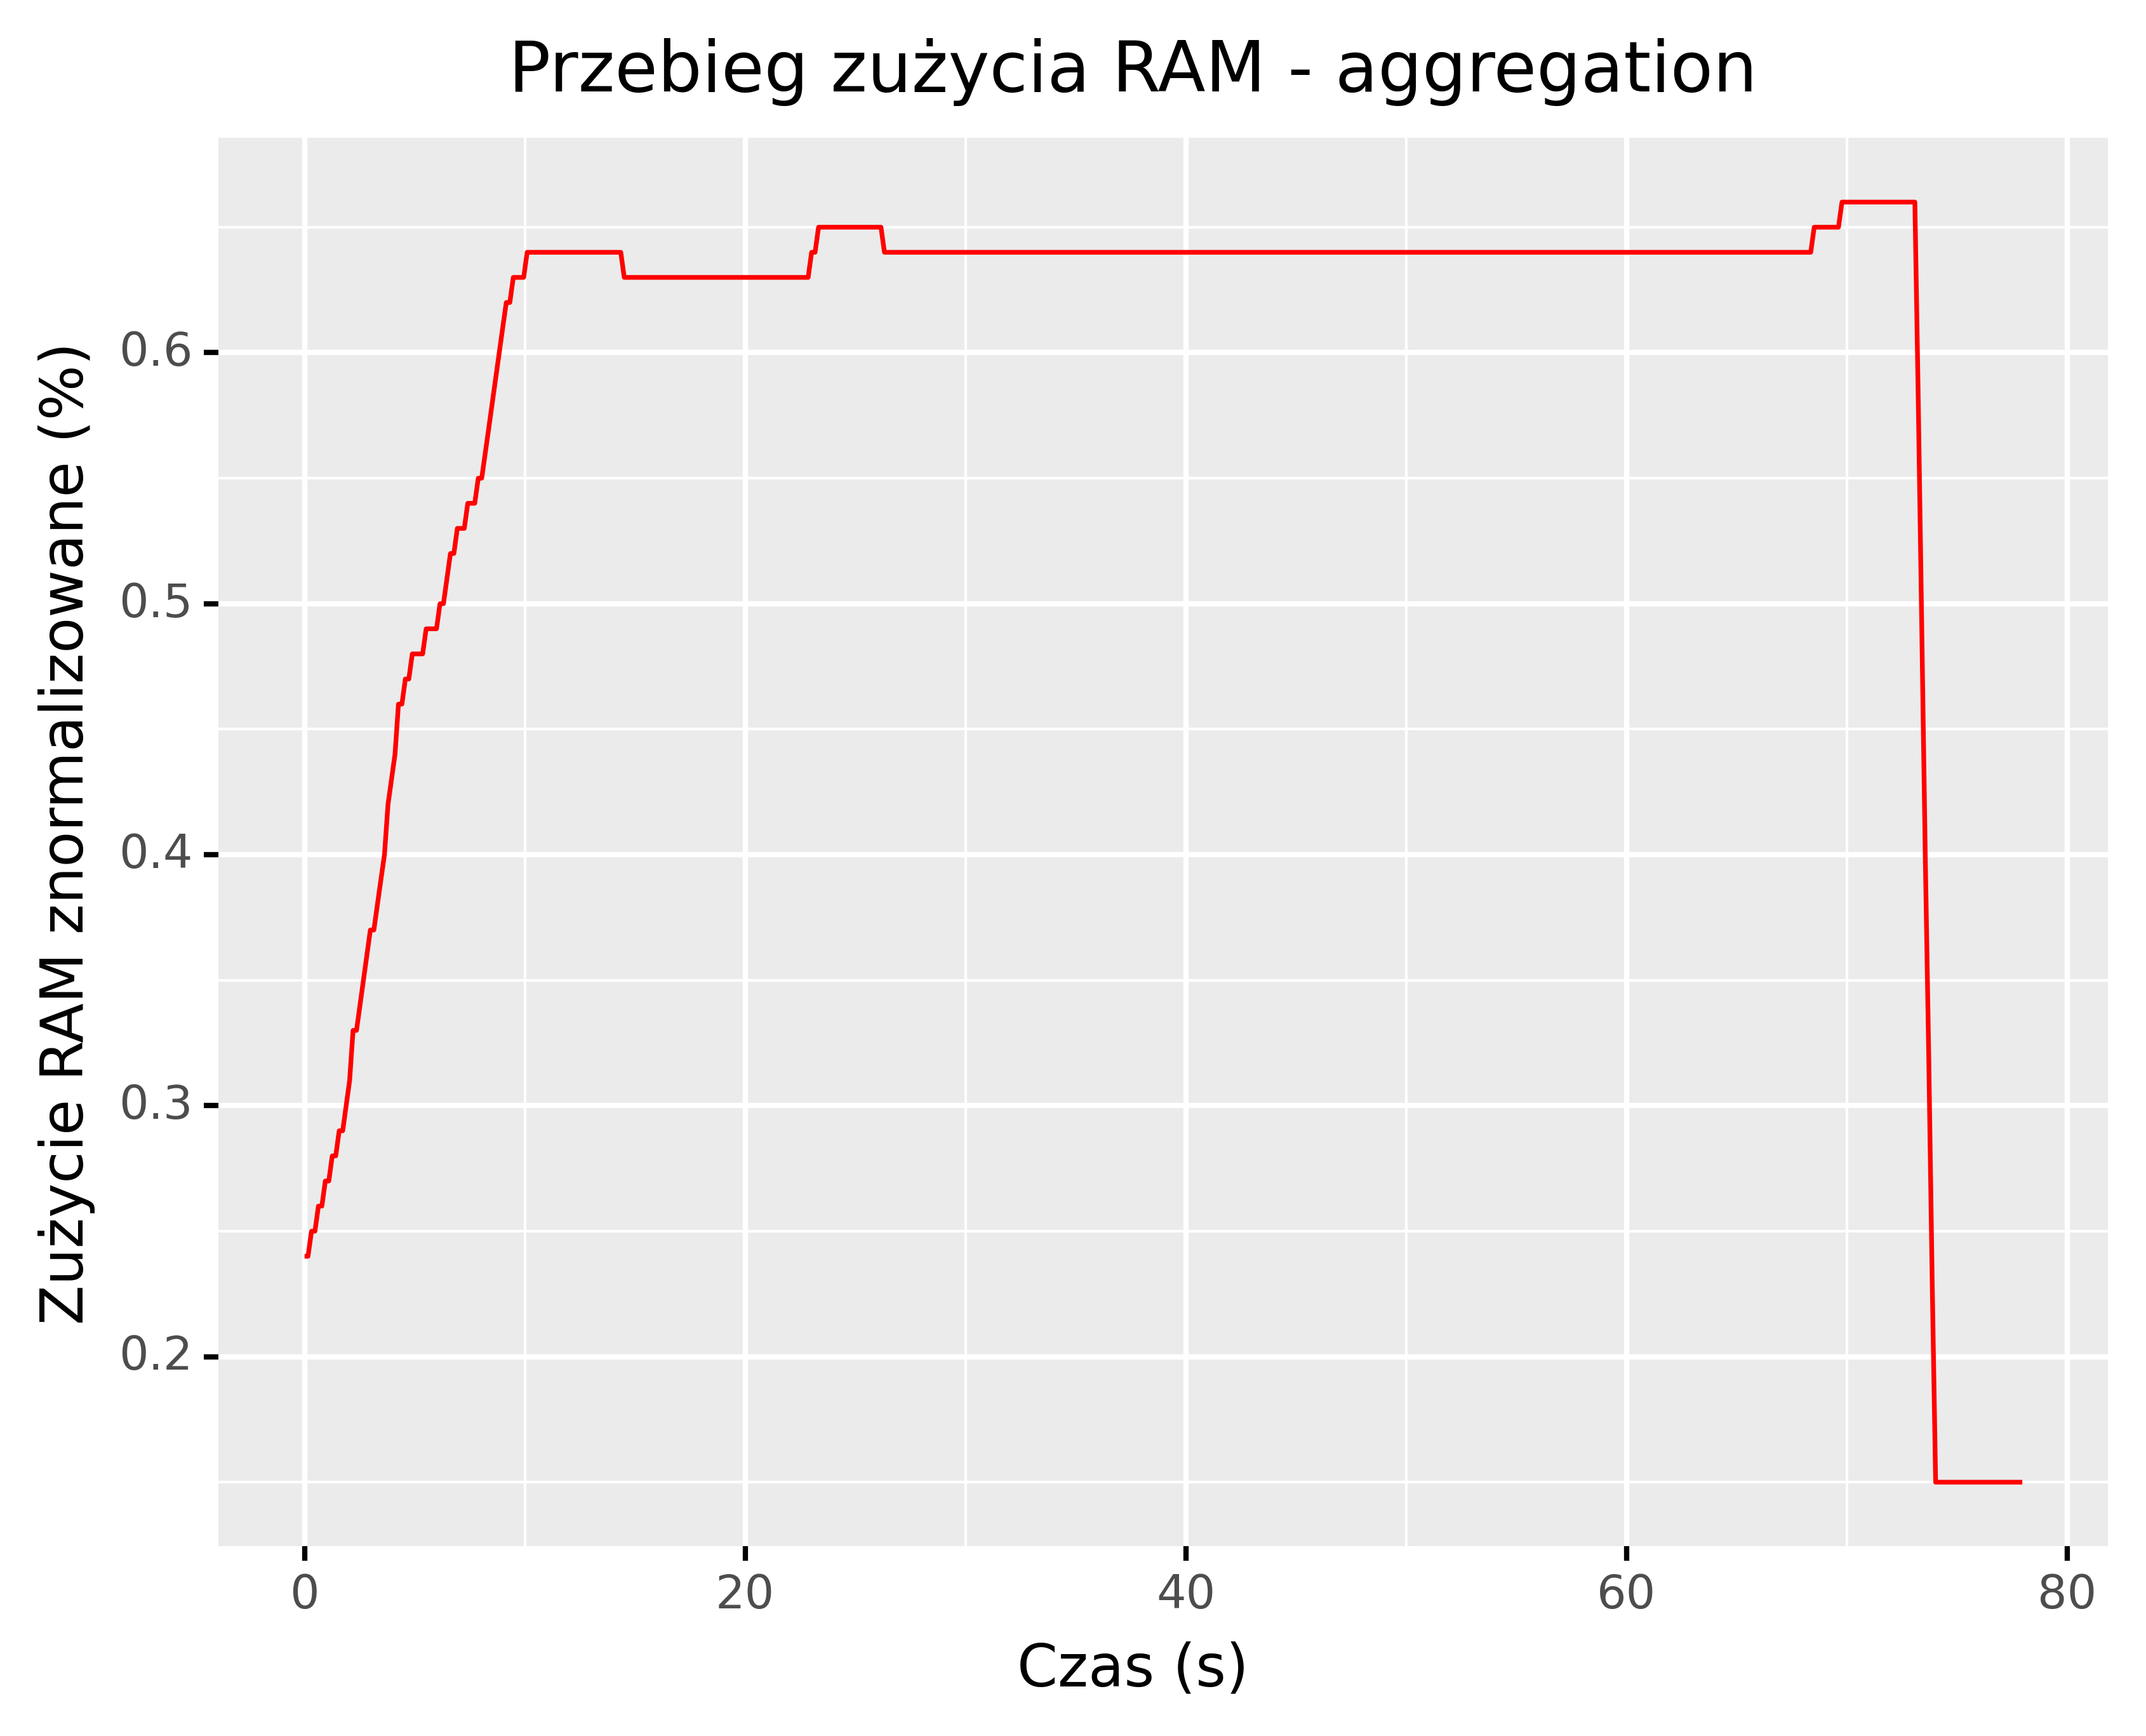
\includegraphics[width=0.5\textwidth]{figures/04-opis-danych/aggregation_smooth_normalized_ram_snapshot_1.png}\label{aggregation_normalized:ram}}
  \caption{Przykładowy znormalizaowany wykres zużycia zasobów dla agregacji (snapshot = 1))}
  \label{aggregation_normalized}
\end{figure}

Na wykresach \ref{aggregation_normalized} widać że po wykonaniu normalizacji kształt wykresów się nie zmienił (porównując z \ref{aggregation_smooth_6}), jednak amplitudy zmalały. W ten sposób przygotowane dane zostaną wykorzystane w eksperymentach, sprawdzając ich skuteczność przed i po normalizacji.

% Co z tymi rozdziałami poniżej?

\section{Charakterystyka danych wejściowych}

% Opisanie podziału na wielkość danych, ilość nodeów (używamy 1), różne funkcje w ramach klasy, przed i po normalizacji, przed i po wygładzeniu etc.
% Typ szeregu (Multivariate non-equal length)
Dla każdej funkcji UDF przygotowano sześć konfiguracji klastra. Na każdej konfiguracji wykonano dwadzieścia pięć eksperymentów. W konfiguracji ustawiano dwie zmienne - wielkość przetwarzanych danych oraz liczbę węzłów. Skutkiem takich ustawień było następujące sześć grup eksperymentów: \begin{itemize}
    \item Rozmiar danych: 1GB, 5 Węzłów
    \item Rozmiar danych: 1GB, 7 Węzłów
    \item Rozmiar danych: 1GB, 9 Węzłów
    \item Rozmiar danych: 2GB, 5 Węzłów
    \item Rozmiar danych: 2GB, 7 Węzłów
    \item Rozmiar danych: 2GB, 9 Węzłów
\end{itemize}
Liczba węzłów nie wpłynęła znacząco na szeregi, gdyż usunięto węzły pełniące rolę mastera oraz węzły nieaktywne.
Rozmiar przetwarzanych danych wpływa jednak istotnie na długość wykonywania się funkcji, a co za tym idzie na część wykorzystywanych algorytmów.
Dodatkowo nawet biorąc pod uwagę identyczną konfigurację dla dwóch kolejnych eksperymentów dotyczącą tej samej funkcji, długość szeregów czasowych okazała się zmienna.
Biorąc pod uwagę wszystkie pliki wynikowe dotyczące agregacji łatwo rozpoznać kolejno długości szeregu dla 1 GB i dla 2 GB danych, dla 12 funkcji, które określone zostały jako agregacja.
\begin{figure}[H]
    \centering
    \captionsetup{justification=centering,margin=0.5cm}
    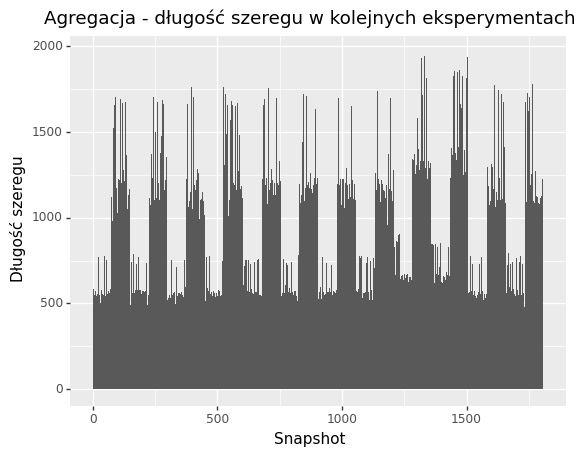
\includegraphics[scale=0.9]{figures/04-opis-danych/data-analysis/AgregacjaDlgSzereguNaSnapshot.png}
    \caption{Agregacja - długość szeregu/snapshot}
    \label{fig:scr46}
\end{figure}
Analiza kolejnych typów funkcji wykazała, że długość szeregu jest jedną z cech różniących typy od siebie. Szczególnie odróznia ona filtrację oraz filtrację-join od pozostałych typów funkcji.
\begin{figure}[H]
    \centering
    \captionsetup{justification=centering,margin=0.5cm}
    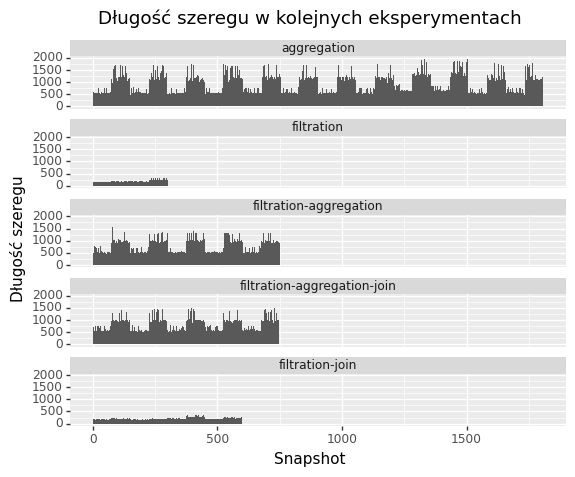
\includegraphics[scale=1.0]{figures/04-opis-danych/data-analysis/all_count.png}
    \caption{Długość szeregu/snapshot}
    \label{fig:scr46}
\end{figure}
Dla dokładniejszej oceny danych przeanalizowano również maksymalne wartości RAM i CPU kolejnych snapshotów dla danego typu funkcji. Na przykładzie agregacji można zauważyć, że dla CPU wartości były różne, jednak większość trzymała się w zakresie 340-390. Było jednak kilka wartości odstających o zdecydowanie mniejszej wartości
\begin{figure}[H]
    \centering
    \captionsetup{justification=centering,margin=0.5cm}
    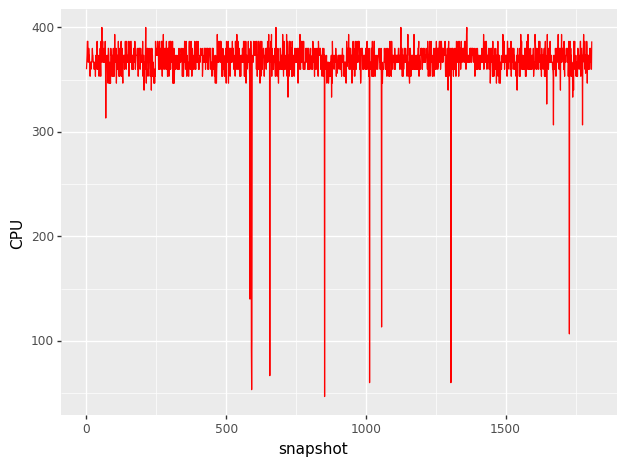
\includegraphics[scale=0.9]{figures/04-opis-danych/data-analysis/aggregation_max_cpu.png}
    \caption{Agregacja - Maksymalne CPU/snapshot}
    \label{fig:scr46}
\end{figure}
Po analizie podobnego wykresu, tylko dotyczącego RAM, okazało się że wartości odstające są tu w tych samych miejscach
\begin{figure}[H]
    \centering
    \captionsetup{justification=centering,margin=0.5cm}
    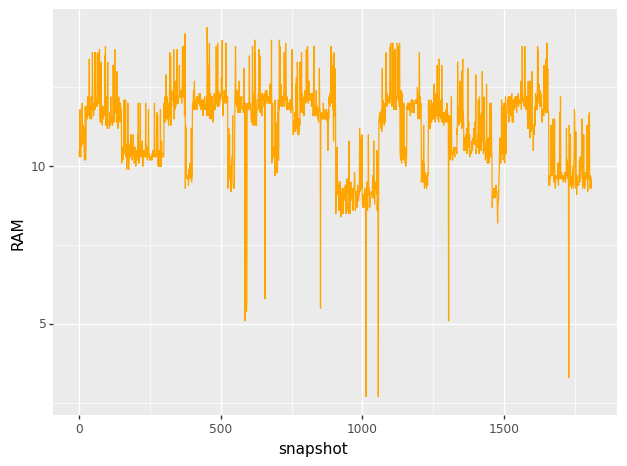
\includegraphics[scale=0.9]{figures/04-opis-danych/data-analysis/aggregation_max_ram.png}
    \caption{Agregacja - Maksymalny RAM/snapshot}
    \label{fig:scr46}
\end{figure}
\begin{figure}[H]
    \centering
    \captionsetup{justification=centering,margin=0.5cm}
    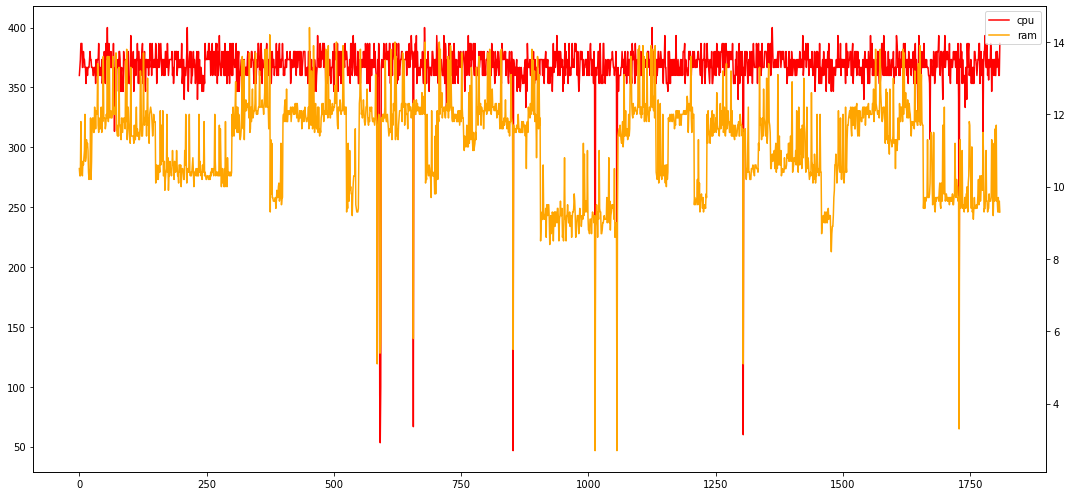
\includegraphics[scale=0.4]{figures/04-opis-danych/data-analysis/aggregation_max_ram_cpu.png}
    \caption{Agregacja - Maksymalny RAM oraz CPU/snapshot}
    \label{fig:scr46}
\end{figure}
Pozostałe typy funkcji miały podobne maksymalne wartości. Miały też w większości przynajmniej jedną wartość odstającą.
\begin{figure}[H]
    \centering
    \captionsetup{justification=centering,margin=0.5cm}
    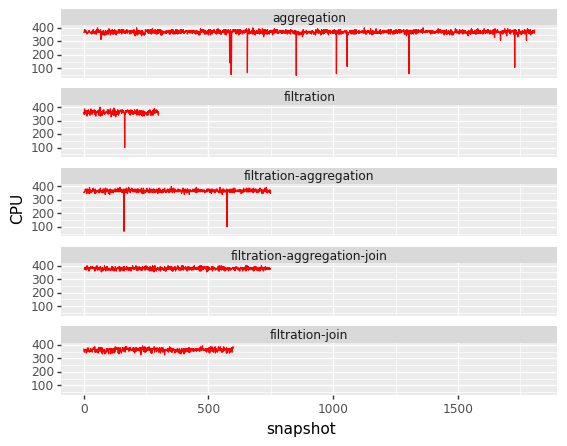
\includegraphics[scale=1.0]{figures/04-opis-danych/data-analysis/all_max_cpu.png}
    \caption{Maksymalne CPU/snapshot}
    \label{fig:scr46}
\end{figure}
\begin{figure}[H]
    \centering
    \captionsetup{justification=centering,margin=0.5cm}
    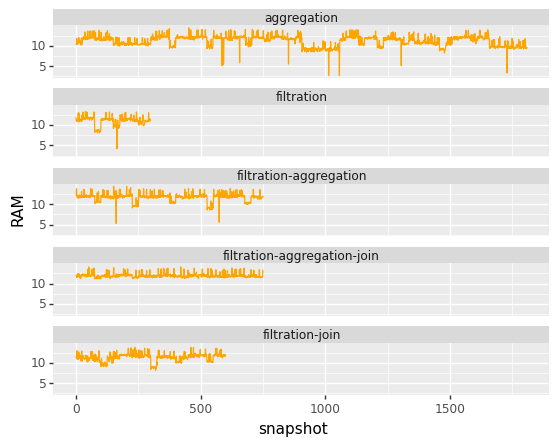
\includegraphics[scale=1.0]{figures/04-opis-danych/data-analysis/all_max_ram.png}
    \caption{Maksymalny RAM/snapshot}
    \label{fig:scr46}
\end{figure}

Przeanalizowane zostały również wartości średnie CPU i RAM. Największe różnice między funkcjami zaobserwowano dla wartości średniej CPU. Widać, że funkcje zawierające agregacje zużywają średnio mniej CPU niż filtracja i filtracja-join. Dodatkowo warto zaobserwować, że jeśli chodzi o agregacje, filtracje-agregacje oraz filtracje-agregacje-join wartości średie są bardzo regularne. Spadki i wzrosty wynikają głównie z tego, że każda funkcja występuje w wersji 1GB i 2GB. Nie dzieje się tak jednak z filtracją. Filtracja jest przedstawiona w zbiorze danych za pomocą jedynie dwóch UDF: filterCatalogSalesWhereProfitNegative i filterStoreSalesWhereProfitNegative. Wyraźnie widać, że jedna z nich używa więcej CPU od drugiej. Może to powodować trudności w identyfikacji filtracji w dalszych rozdziałach pracy.
\begin{figure}[H]
    \centering
    \captionsetup{justification=centering,margin=0.5cm}
    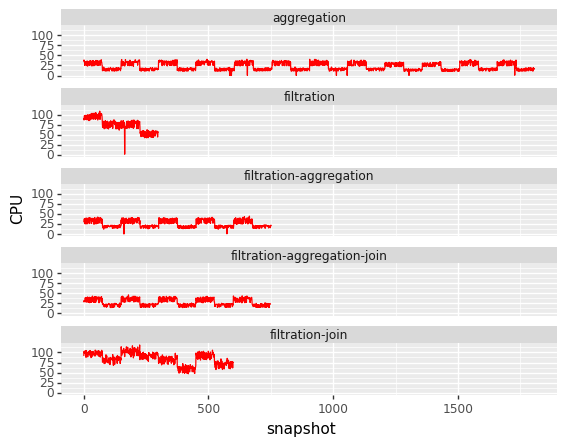
\includegraphics[scale=1.0]{figures/04-opis-danych/data-analysis/all_mean_cpu.png}
    \caption{Średnia CPU/snapshot}
    \label{fig:scr46}
\end{figure}
\begin{figure}[H]
    \centering
    \captionsetup{justification=centering,margin=0.5cm}
    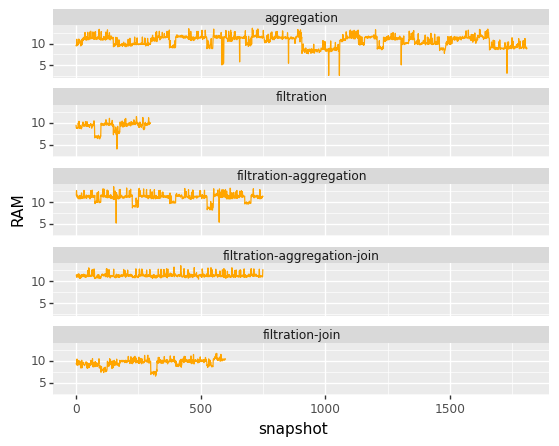
\includegraphics[scale=1.0]{figures/04-opis-danych/data-analysis/all_mean_ram.png}
    \caption{Średnia RAM/snapshot}
    \label{fig:scr46}
\end{figure}

\section{Cechy danych w kontekście wyboru algorytmu}
Podsumowując, analiza danych wykazała, że porównując funkcje między sobą należy spodziewać się pojedynczych wartości odstających. Zostało również odkryte, że jedną z ważniejszych różnic między typami funkcji jest czas wykonywania, a co za tym idzie długość szeregu czasowego. Dodatkowo tak jak maksymalne wartości zużycia CPU i RAMu były podobne dla każdego typu, tak średnia CPU różniła się znacząco między typami. Na tej podstawie wyciągnięto kilka wniosków co do wyboru algorytmów porównywania szeregów czasowych.
\begin{itemize}
    \item Fakt pojawiania się wartości odstających może negatywnie wpływać na rozróżnianie UDFów za pomocą odległości Euklidesowej. Z drugiej strony to, że długość szeregów czasowych potrafi przynajmniej częściowo determinować typ funkcji sprawia, że jest to algorytm warty rozważenia. Problematyczne będą jednak przypadki porównywania dwóch identycznych funkcji, ale użytych na różnych rozmiarach danych.
    \item Algorytm Dynamic Time Warping jest stworzony do radzenia sobie ze skalowaniem czasu. Jest to pozytywny efekt, gdy patrzy się na to że celem jest między innymi dopasowanie wyników, które powstały przy użyciu danych o różnych rozmiarach, w tym przypadku rozmiary to 1GB i 2GB, jednak fakt pracy na różnych rozmiarach danych byłby rzeczą naturalną, gdyby chcieć wykorzystać omówione algorytmy do rzeczywistej analizy UDF. Z drugiej strony czas wykonania jest tym co wyraźnie odróżnia część algorytmów od siebie, rezygnacja z tej informacji niekoniecznie jest dobrym rozwiązaniem. 
    \item Algorytm Landmark Similarity również radzi sobie ze skalowaniem czasu, ale też skalowaniem amplitudy. Zwraca uwagę niemal wyłącznie na kształt wykresu. Jest to problematyczne w przypadku omawianym w tej pracy, gdyż zarówno amplituda jak i długość szeregu przekazuje dużo informacji o typie funkcji. 
\end{itemize}